\documentclass[11pt,a4paper,titlepage,twoside]{book}
\usepackage{pdflscape}
%\usepackage[textwidth=450pt]{geometry}
\usepackage[left=0.8in,right=0.8in,top=1in,bottom=0.7in]{geometry}
\usepackage{graphicx}
\usepackage{lastpage}
\usepackage{amsmath,amssymb,amsthm}
\usepackage{eqlist}
\usepackage{array}
\usepackage{thmbox}
\usepackage{multirow}
\usepackage{comment}
\setlength{\parskip}{8pt plus 2pt minus 2pt}
\setlength{\parindent}{0pt}
\usepackage{fancyhdr}
\usepackage{pdfpages}
\usepackage{minitoc}
\usepackage{timetable}
\usepackage{longtable}
\usepackage{xeCJK}
\usepackage{comment}
\usepackage{titletoc}
\usepackage{titlesec}
\usepackage{unnumberedtotoc}
\usepackage{ltablex,makecell}
\usepackage[Glenn]{fncychap}
\usepackage{hyperref}
\setCJKmainfont[BoldFont=SimHei]{SimSun}
\usepackage{tikz}
\usetikzlibrary{arrows}
%\usepackage{tabularx,makecell}


\makeatletter
\def\hlinewd#1{%
\noalign{\ifnum0=`}\fi\hrule \@height #1 %
\futurelet\reserved@a\@xhline}
\makeatother

% %Options: Sonny, Lenny, Glenn, Conny, Rejne, Bjarne, Bjornstrup

\graphicspath{{figures/}}

\pagestyle{fancy}
\fancyhead{} 
\lhead{SPHERIC Beijing 2017}
\chead{}
\rhead{Beijing, China, October 17-20, 2017} 


\makeatletter
\renewcommand*{\cleardoublepage}{\clearpage\if@twoside \ifodd\c@page\else
\hbox{}%
\thispagestyle{empty}%
\newpage%
\if@twocolumn\hbox{}\newpage\fi\fi\fi}
\makeatother

\newcommand\MBLiu{\href{http://www.coe.pku.edu.cn/dept/f/Liu-Moubin}{Moubin Liu}}

\begin{document}
%\title{2017 SPHERIC Beijing International Workshop\\Conference Handbook}
%\author{Peking University}
%\date{October, 17-20, 2017}
%\maketitle

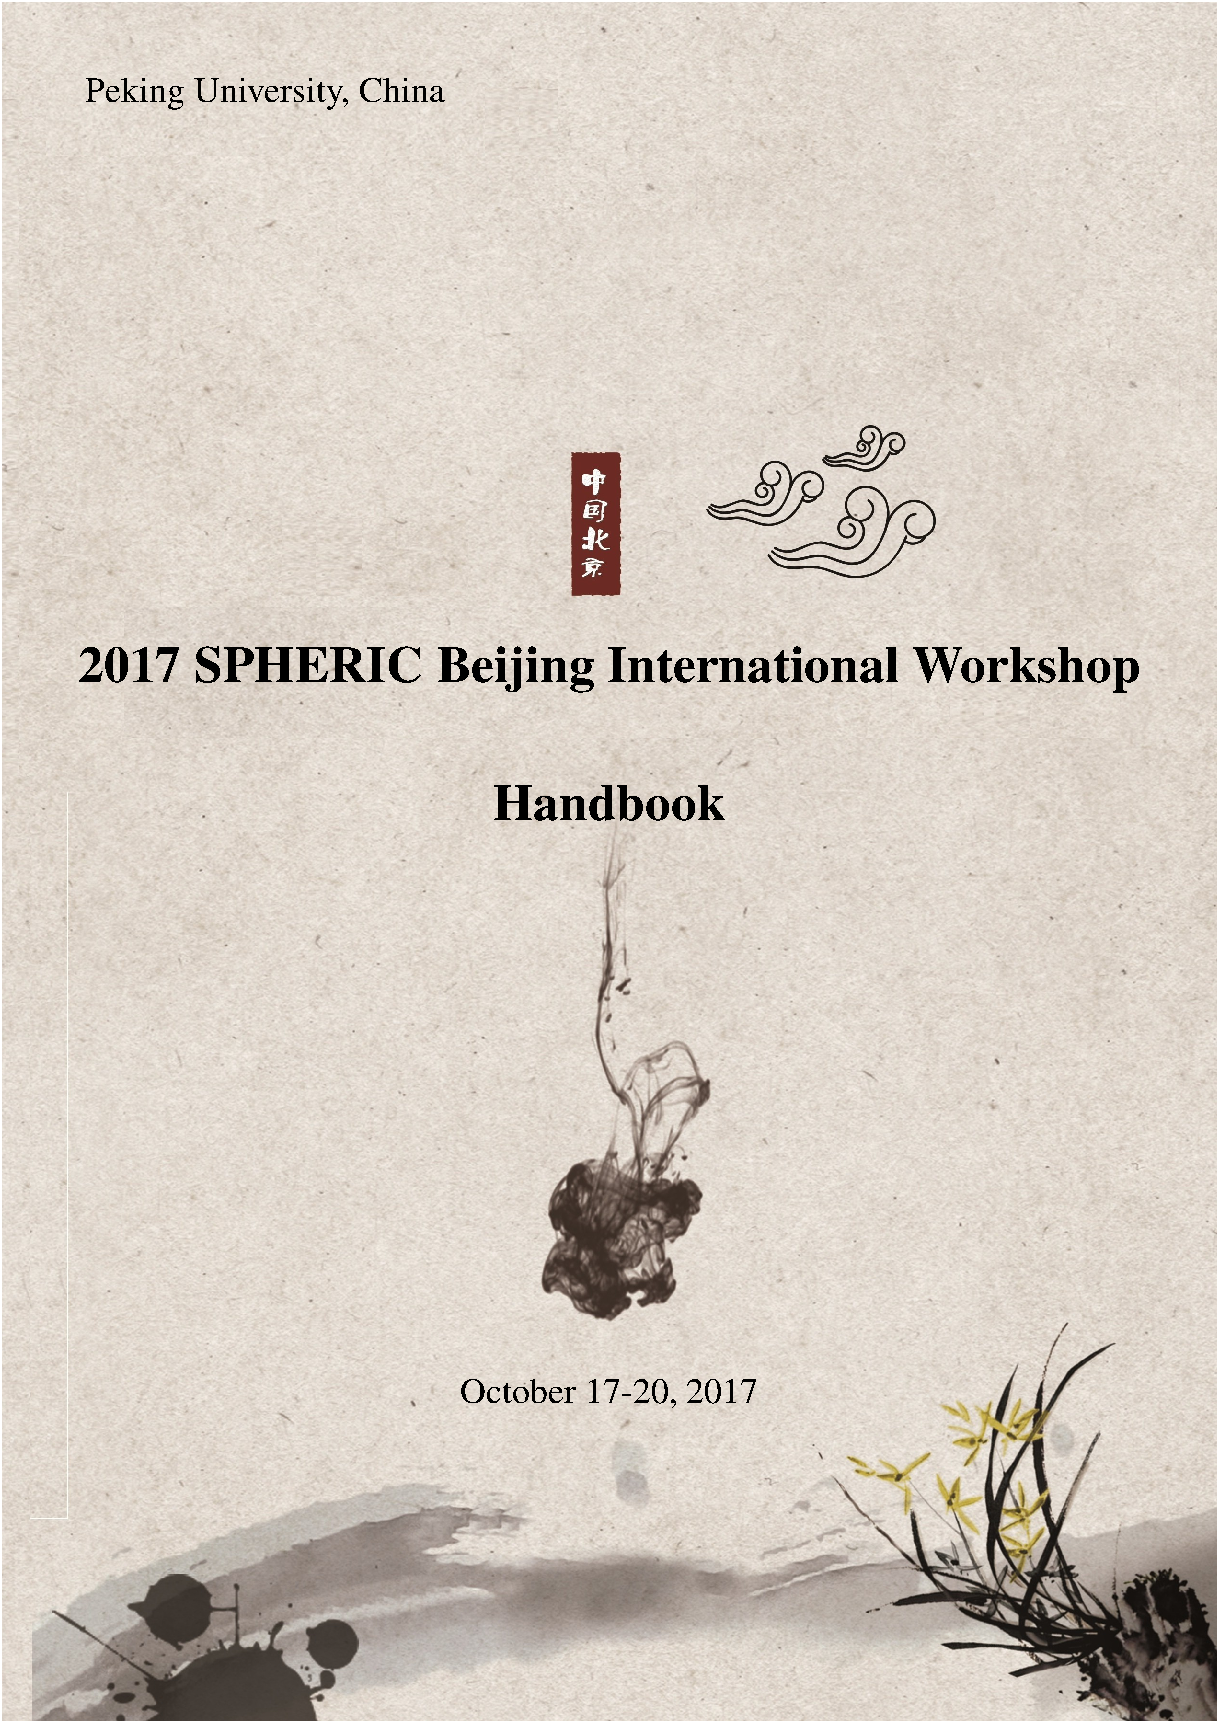
\includepdf{figures/coverA-print.pdf}

\cleardoublepage

\pagenumbering{roman}

\newgeometry{left=0.8in,right=0.8in,top=0in,bottom=0.7in}
\chapter*{Welcome Message}
%\addchap{Welcome Message}
%\addstarredchapter{Welcome Message}
%\chaptermark{Welcome Message}
%\addcontentsline{toc}{chapter}{Welcome Message} \mtcaddchapter

\vspace{-5em}
\textbf{\Large Dear Delegates}\vspace{1em}

The College of Engineering of Peking University is delighted to host the 2017 SPHERIC Beijing International Workshop (or \textbf{SPHERIC Beijing 2017}). This is an important event of 2017 in the field of Smoothed Particle Hydrodynamics (SPH) and related particle-based methods.

The SPH European Research Interest Community (SPHERIC) was founded in 2005 as a Special Interest Group of the ERCOFTAC community and aims at encouraging and facilitating the spread of the method throughout Europe and the wider international community. Since that time, the SPHERIC community continues both to grow and to play an important role in helping the development of SPH for academia, industry and government organizations. SPH is one of the most exciting new areas in the field of computational methods and is opening up the possibility of research into fields that were beyond any modelling capability. 

The SPHERIC Beijing 2017 organization committee received abstracts from China, France, Germany, UK, Italy, Spain, Switzerland, Ireland, USA, Japan and Australia, while 56 abstracts were selected to present in the SPHERIC Beijing 2017. This demonstrates just how active the field is, with works ranging from traditional hydrodynamics to solids, fluid-structure interaction, high performance computing and industrial applications. 

The SPHERIC Beijing 2017 has been supported by the National Natural Science Foundation of China (NSFC), the Chinese Society of Theoretical and Applied Mechanics (CSTAM), Beijing Innovation Centre for Engineering Science and Advanced Technology (BIC-ESAT), Institute of Ocean Research and State Key Laboratory for Turbulence and Complex Systems of Peking University, and Beijing Paratera Technology Co. Ltd.  

It is a great pleasure to welcome you all to Beijing, and share a successful and enjoyable meeting with you.


\begin{flushright}
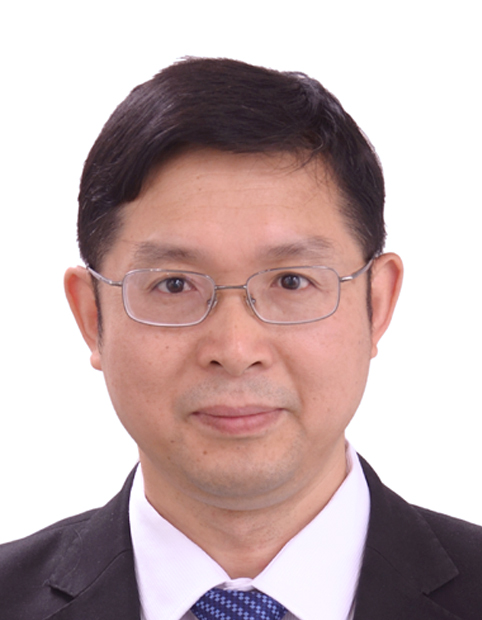
\includegraphics{mbliu.jpg}\\
\textbf{\MBLiu ~~~~~}\\
\vspace{1em}

Professor, Peking University\\
Chair, Local Organization Committee\\
SPHERIC Beijing 2017
\end{flushright}
\newgeometry{left=0.8in,right=0.8in,top=1in,bottom=0.7in}

\chapter*{Acknowledgement}

{\bf\Large SPHERIC Beijing 2017 has been supported by }
\vspace{1.5em}

\begin{minipage}[c]{0.42\linewidth}
\href{http://www.nsfc.gov.cn}{National Natural Science Foundation of China (NSFC)}
\end{minipage}
\begin{minipage}[c]{0.05\linewidth}
~
\end{minipage}
\begin{minipage}[c]{0.5\linewidth}

\includegraphics[width=\textwidth]{NSFC.jpg}
\end{minipage}
\vspace{1em}


\begin{minipage}[c]{0.42\linewidth}
\href{http://www.cstam.org.cn}{Chinese Society of Theoretical and Applied Mechanics (CSTAM)}
\end{minipage}
\begin{minipage}[c]{0.05\linewidth}
~
\end{minipage}
\begin{minipage}[c]{0.5\linewidth}

\includegraphics[width=\textwidth]{CSTAM.png}
\end{minipage}


\vspace{1em}

\begin{minipage}[c]{0.42\linewidth}
\href{http://ocean.pku.edu.cn}{Institute of Ocean Research, Peking University}
\end{minipage}
\begin{minipage}[c]{0.05\linewidth}
~
\end{minipage}
\begin{minipage}[c]{0.5\linewidth}

\includegraphics[width=\textwidth]{Ocean.jpg}
\end{minipage}

\vspace{1em}

\begin{minipage}[c]{0.42\linewidth}
\href{http://www.pku.edu.cn}{Beijing Innovation Centre for Engineering Science and Advanced Technology (BIC-ESAT), Peking University}
\end{minipage}
\begin{minipage}[c]{0.05\linewidth}
~
\end{minipage}
\begin{minipage}[c]{0.5\linewidth}

\includegraphics[width=\textwidth]{BIC-ESAT.jpg}
\end{minipage}

\vspace{1em}

\begin{minipage}[c]{0.42\linewidth}
\href{http://ltcs.pku.edu.cn}{State Key Laboratory for Turbulence and Complex Systems, Peking University}
\end{minipage}
\begin{minipage}[c]{0.05\linewidth}
~
\end{minipage}
\begin{minipage}[c]{0.5\linewidth}

\includegraphics[width=\textwidth]{SKLTCS.png}
\end{minipage}

\vspace{1em}

\begin{minipage}[c]{0.42\linewidth}
\href{http://en.paratera.com}{Beijing Paratera Technology Co. Ltd. }
\end{minipage}
\begin{minipage}[c]{0.05\linewidth}
~
\end{minipage}
\begin{minipage}[c]{0.5\linewidth}

\includegraphics[width=\textwidth]{BPT.png}
\end{minipage}

%\newgeometry{left=0.8in,right=0.8in,top=0in,bottom=0.7in}
\rhead{Contents} 
\setcounter{tocdepth}{1}
\renewcommand\contentsname{CONTENTS}
\dominitoc\tableofcontents
%\newgeometry{left=0.8in,right=0.8in,top=1in,bottom=0.7in}
 
\newpage
\pagenumbering{arabic}

\chapter*{About SPHERIC}\chead{About SPHERIC}
%\addchap{About SPHERIC}
\rhead{About SPHERIC}
%\addstarredchapter{About SPHERIC}
%\chaptermark{About SPHERIC}
\addcontentsline{toc}{chapter}{About SPHERIC} \mtcaddchapter
\vspace{-5em}

SPHERIC, or ``SPH European Research Interest Community'', is the international organisation representing the community of researchers and industrial users of Smoothed Particle Hydrodynamics (SPH), aims to promote the SPH method in both academic and industrial fields and enhance collaborations between countries and institutes. It was recognized as a Special Interest Group (SIG) within Ercoftac in January 2006.

As a purely Lagrangian technique, SPH enables the simulation of highly distorting fluids and solids. Fields including free-surface flows, solid mechanics, multi-phase, fluid-structure interaction and astrophysics where Eulerian methods can be difficult to apply represent ideal applications of this meshless method.

The SPH method was developed to study non-axisymmetric phenomena in astrophysics in the 1970s, but its application to engineering emerged in the 1990s and early 2000s. In the past twenty years the method has developed rapidly in many fields of application from impacts to fracture to breaking waves and fluid-structure interaction.

Following the impulse generated by a collection of local initiatives in 2005 (France, UK, Italy...), a need to foster and collaborate efforts and developments was identified. Since then, the SPHERIC organisation has gone on to push the development of the method forward providing a network of researchers and industrial users around the world as a means to communicate and collaborate.

For more information about SPHERIC, please visit \url{http://spheric-sph.org}

\vspace{2em}
\textbf{\Large SPHERIC Beijing 2017}

%\addcontentsline{toc}{section}{SPHERIC Beijing 2017}
You are cordially invited to attend the 2017 SPHERIC Beijing International Workshop (SPHERIC Beijing 2017) to be held at Peking University (PKU) in Beijing China, from October, 17-20, 2017. This is the first time that the SPHERIC Workshop is held outside Europe.

The SPHERIC workshops are the only worldwide events which exclusively focus on the Smoothed Particle Hydrodynamics (SPH) methodology and related simulation approaches. SPH has recently gained enhanced attention in the area of scientific computing. Exemplary applications refer to the development of galaxies in astrophysics, environmental engineering, applied solid mechanics, marine and coastal engineering, nuclear power engineering, medical engineering or geotechnical problems.

The successful concept of SPHERIC is due to a methodological focus in an interdisciplinary application environment, integrating the know-how of physicists, mathematicians, IT experts and engineers from academia and industry. On behalf of the organizing team, it is a pleasure and honor to us to invite scientists and researchers to the SPHERIC 2017 at PKU, in Beijing, China.

For more information about SPHERIC Beijing 2017, please visit \url{http://ocean.pku.edu.cn/SPHERIC_Beijing/index.php.htm}
\chapter*{About Peking University} 
%\addchap{About Peking University}
\rhead{About PKU}
%\addstarredchapter{About Peking University}
%\chaptermark{About Peking University}
\addcontentsline{toc}{chapter}{About Peking University}\mtcaddchapter
\vspace{-5em}

\section*{General Information}
%\addcontentsline{toc}{section}{General Information} 
Peking University is a comprehensive and national key university. The campus, known as "Yan Yuan"(the garden of Yan), is situated at Haidian District in the western suburb of Beijing, with a total area of 2,743,532 square metres (or 274 hectares). It stands near to the Yuanmingyuan Garden and the Summer Palace.

Peking University is proud of its outstanding faculty, including 53 members of the Chinese Academy of Sciences (CAS), 7 members of the Chinese Academy of Engineering (CAE), and 14 members of the Third World Academy of Sciences (TWAS).

The university has effectively combined research on important scientific subjects with the training of personnel with a high level of specialized knowledge and professional skill as demanded by the country's socialist modernization. It strives not only for improvements in teaching and research work, but also for the promotion of interaction and mutual promotion among various disciplines.  

Thus Peking University has become a center for teaching and research and a university of a new type, embracing diverse branches of learning such as basic and applied sciences, social sciences and the humanities, and sciences of medicine, management, and education. Its aim is to rank among the world's best universities in the future. 

\section*{History}
%\addcontentsline{toc}{section}{History}
Founded in 1898, Peking University was originally known as the Imperial University of Peking. It was the first national university covering comprehensive disciplines in China, and has been a leading institution of higher education in China since its establishment. It also served as the highest administration for education at the beginning of its founding. 


In 1912, the university adopted its present name. At the end of the 20th century, the Chinese government put Peking University at the top of its agenda for promoting higher education, with the aim to build a world-class university in the 21st Century. After merging with Beijing Medical University in 2000, Peking University once again was strengthened in its disciplinary structure. 

Peking University has continually played the essential role of pioneers in the course of China's modernization. The university's traditional emphasis on patriotism, progress, democracy, and science, together with its educational standards of diligence, precision, factualism, and innovation, have been passed down from generation to generation. 

%\vspace{3.25em}
%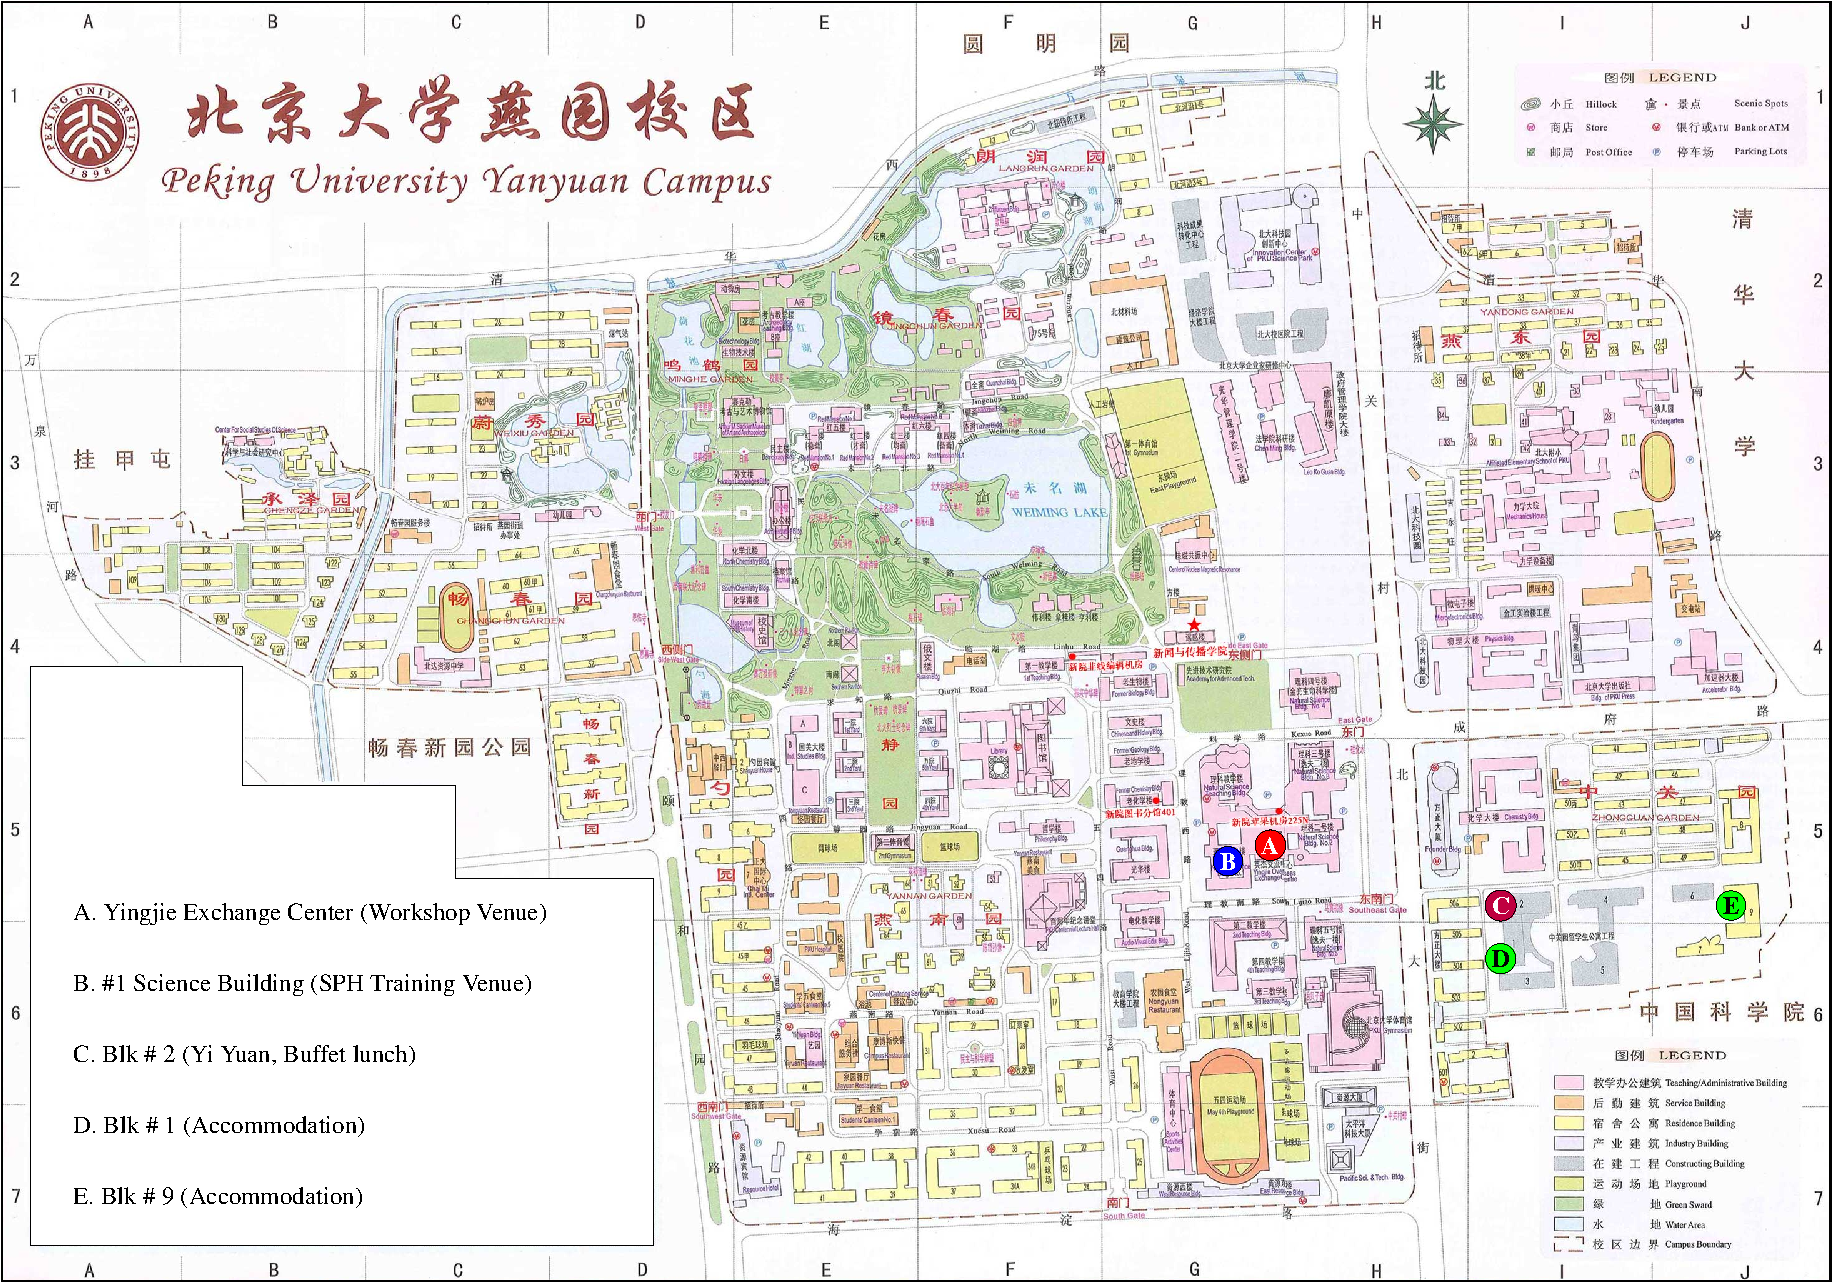
\includegraphics[width=\textwidth]{PKU.jpg}

%\setlength{\parskip}{2.5pt plus 2pt minus 2pt}

\chapter*{Workshop Details}
\chead{Workshop Details}
%\addstarredchapter{About SPHERIC}
%\chaptermark{About SPHERIC}
\addcontentsline{toc}{chapter}{Workshop Details} \mtcaddchapter
\vspace{-5em}




\phantomsection
\addsec{Committees}\rhead{Committees}

\subsection*{Scientific Committee}\vspace{-1em}
%\addcontentsline{toc}{section}{Scientific Committee} 
\begin{itemize}
\item Prof. David Le Touz\'e (Ecole Centrale de Nantes, France)
\item Dr. Damien Violeau (Electricit\'e de France, France)
\item Dr. Nathan Quinlan (National Univ. of Ireland, Ireland)
\item Dr. Ben Rogers (University of Manchester, UK)
\item Prof. Stefano Sibilla (University of Pavia, Italy)
\item Dr. Jean-Christophe Marongiu (ANDRITZ Hydro, France)
\item Dr. Alex Crespo (Universidade de Vigo, Spain)
\item Dr. Andrea Colagrossi (INSEAN, Italy)
\item Dr. Xiangyu Hu (Technical University of Munich, Germany)
\item Prof. Rade Vignjevic (Brunel University of London, UK)
\item Prof. Thomas Rung (Technical University of Hamburg-Harburg, Germany)
\item Dr. Antonio Souto-Iglesias (Technical University of Madrid, Spain)
\item Dr. Renato Vacondio (University of Parma, Italy)
\item Dr. Matthieu De Leffe (Nextflow Software, France)
\item Prof. Moncho G\'omez-Gesteira (Universidade de Vigo, Spain)
\item Dr. Abbas Khayyer (University of Kyoto, Japan)
\item Prof. Walter Dehnen (University of Leicester, UK)
\item Dr. Raj Das (University of Auckland, New Zealand)
\item Prof. Robert A. Dalrymple (Johns Hopkins University , USA)
\item Prof. Alexis H\'erault (Conservatoire National des Arts et M\'etiers, France)
\item Prof. Joe Monaghan (Monash University, Australia)
\item Prof. Peter Eberhard (University of Stuttgart, Germany)
\item Prof. Moubin Liu (Peking University, China)
\item Dr Mehmet Yildiz (Sabanci University, Turkey)
\end{itemize}



\subsection*{Organizing Committee}
%\addcontentsline{toc}{section}{Organizing Committee} 
\subsubsection*{Chair}\vspace{-1em}
\begin{itemize}
\item Prof.   M. B. Liu, Peking University
\end{itemize}

\subsubsection*{Co-Chairs}\vspace{-1em}
\begin{itemize}
\item Prof.   H. F. Qiang, Xi'an Hi-Tech Institute, China
\item Prof.   A. M. Zhang, Harbin Engineering University, China
\item Prof.   L. Zou, Dalian University of Technology, China
\item Prof.   D. A. Hu, Hunan University, China
\item Prof.   F. Xu, Northwestern Polytechnical University, China
\item Prof.   Z. R. Li, Wenzhou University, China
\end{itemize}


\newpage
\phantomsection
\addsec{Keynote Speakers}
\rhead{Keynote Speakers}
\phantomsection
\subsection*{Prof.  David Le Touzé}\label{David}
\textit{Ecole Centrale Nantes}\\
\textit{Deputy Head, LHEEA research dept. (ECN and CNRS)}\\
\textit{Head, H2I research group of LHEEA}\\
\textit{Head, Centrale Nantes - Bureau Veritas Chair}\\
\textit{Head, IRT Jules Verne SimAvHy Chair}

\textbf{Title}: Smoothed Particle Hydrodynamics, fact checking: from theory to applications

%\textbf{Abstract}: An overview of the Smoothed Particle Hydrodynamics applied to free-surface and interface flows is provided in the talk, under the form of fact checking. The complex links between the Lagrangian feature of the method, the smoothed and discretized operators, the modeling of physical terms and boundary conditions, on the one hand, and the conservation, convergence and accuracy of the method, on the other hand, are discussed. The links between the physical modeling of free-surface conditions and incompressibility, and the time solving and HPC implementation of the method are also explored. This current understanding of the SPH method permits to highlight the current successful SPH schemes, their accuracy, efficiency, limitations and target types of applications. A set of example successful industrial engineering applications is presented. The interest and feasibility of coupling to other methods is also highlighted.

\textbf{Bio}: Prof. David LE TOUZÉ is 40 years old. He got his MSc in Hydrodynamics and Ocean Engineering from Ecole Centrale Nantes (Nantes, France) in 2000. Ecole Centrale Nantes is a highly competitive French « Grande Ecole » which awards MScs and PhDs only. He then got his PhD with honors in 2003 from the same institute, whose topic was modeling gravity wave generation and propagation by spectral methods. He spent 2 years of post-doc at CNR-INSEAN (Rome, Italy) in 2004-05 where he started working in SPH. He came back to Ecole Centrale Nantes in 2006 and became Assistant Professor in 2007, Associate Professor in 2010 and Full Professor in 2012. His researches revolve mainly around free-surface flows. He is leading since 2012 a research group on Hydrodynamics, Interfaces and Interactions (H2i) which counts 8 professors and researchers, 14 PhD students, and 6 post-docs. His current research topics cover different numerical methods and techniques: SPH (Smoothed Particle Hydrodynamics), incompressible (OpenFOAM) and weakly-compressible (WCCH) Finite Volumes, Adaptive Mesh Refinement (AMR), Immersed Boundary Method (IBM), Vortex Method (DVH), Lattice-Boltzmann Method (LBM). He is also working on different method couplings: potential (waves) to Navier-Stokes Finite Volume Method for wave-structure interactions, SPH to Finite Element Method (FEM) for fluid-structure interaction, SPH to Finite Volume Method for efficient solutions of complex flows. Main applications of his research are in the fields of marine engineering (many naval, offshore and marine renewable energy topics), automotive (aquaplaning, gear boxes), aeronautics (ditching) and health (cardio-vascular flows). He is currency leading 7 industrial projects (over 5M contracts). He is the author of 30+ journal publications, with a google h-index of 22. He is also Deputy Head of his research department (LHEEA, 140 staff) which is a joint research unit between Ecole Centrale Nantes and CNRS.

\phantomsection
\subsection*{Prof.  J. S. Chen}\label{Chen}
\textit{William Prager Chair Professor, Structural Engineering Department, Director, Center for Extreme Events Research, University of California, San Diego}

\textbf{Title}: An Implicit Gradient Reproducing Kernel Particle Method: Theory and Applications

%\textbf{Abstract}: High strain rate events such as projectile penetration and blast often result in fragmentation, complex contact conditions, and severe material damage. The Reproducing Kernel Particle Method (RKPM) relies on nodal integration to yield a pure point-based method for effective simulation of these events, however stability of nodal integration is difficult to achieve without upsetting computational efficiency or introducing user-tuneable parameters. In this work, a naturally stabilized nodal integration method is formulated under a strain-smoothing framework, and a variational consistency correction for nodal integration is introduced to ensure optimal convergence. Taylor expansion of nodal strains in conjunction with implicit gradients yields high computational efficiency, with stabilization constants naturally arising as moments of inertia of nodal domains. The method is cast under a strain smoothing framework to achieve additional stability in extreme event modelling, with the benefit of further enhancing computational efficiency. Simulation of blast and penetration events will be presented to demonstrate the effectiveness of the proposed method.

\textbf{Bio}: J. S. Chen earned his undergraduate degree from National Central University (1978-1982) in Taiwan, and received master's (1986) and Ph.D. (1989) from Northwestern University. He worked in GenCorp's Research Division from 1989 to 1994. From 1994 to 2001, he held a faculty position in the Mechanical Engineering Department of The University of Iowa before moving to UCLA in 2001, where he served as the Chair of Civil \& Environmental Engineering Department from 2007 to 2012. He was the Chancellor's Professor in the Civil \& Environmental Engineering Department at UCLA and also Professor of Mechanical \& Aerospace Engineering Department and Mathematics Department. In 2013, he joined the Structural Engineering Department of UCSD as the inaugural holder of the William Prager Endowed Chair. He also is the director of the Center for Extreme Events Research at the Jacobs School of Engineering at UC San Diego.




\newpage
\phantomsection
\addsec{Conference Venue}\rhead{Conference Venue}
The SPHERIC Beijing 2017 will be held at Peking University, Beijing, China.
\begin{itemize}
\item Address: No.5 Yiheyuan Road Haidian District, Beijing, P.R.China 
\item Tel:  +86 1062 766 982
\item Website: \url{http://ocean.pku.edu.cn/SPHERIC_Beijing/index.php.htm}
\end{itemize}

\phantomsection
\addsec{Accommodation}
\textbf{For participants outside China}, the committee has reserved rooms at \textbf{ZhongGuanYuan Global Village PKU} at discounted prices. It should be noted that the registration fee does not include accomodation. All of the hotels below include breakfast and wifi access. 
\begin{itemize}
\item Address: No.126 ZhongGuanCun North Street, Haidian District, Beijing, China
\item Tel:  +86 10 62752288
\item Website: \url{http://www.pkugv.com}
\end{itemize}

\phantomsection
\addsec{Transportation Information}
TAXI Taxi is the most convenient transportation to the University from the airport. As the Capital Airport is located 40 km northeast from the campus, it will cost you around 100-130 RMB (expressway fee of 15 RMB included) to get to the university from the airport. It takes approximately 1-1.5 hours to arrive at PKU from the airport, depending on the traffic.

Getting to PKU from the Airport BUS You may also first travel to ZhongGuanCun via the airport shuttle bus and then take a taxi from ZhongGuanCun.

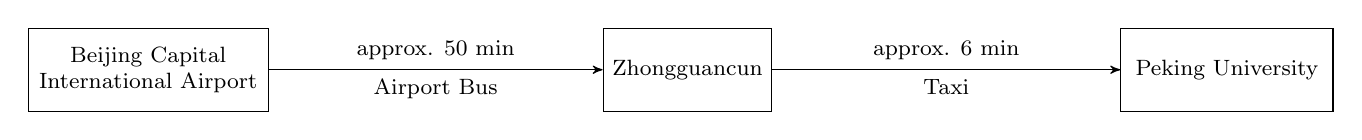
\begin{tikzpicture}[font=\footnotesize]
\node(zgc)[shape=rectangle,draw,minimum height=3em] at (0,0){Zhongguancun};
\node(cia)[shape=rectangle,draw,text width=8em,text centered, minimum height=3em] at (-6.85,0){Beijing Capital\\ International Airport};
\node(pku)[shape=rectangle,draw,text width=7em,text centered, minimum height=3em] at (6.85,0){Peking University};
\draw[->,>=stealth'] (cia)--(zgc) node[midway,above]{approx. 50 min} node[midway,below]{Airport Bus};
\draw[->,>=stealth'] (zgc)--(pku) node[midway,above]{approx. 6 min} node[midway,below]{Taxi};
\end{tikzpicture}


You may also take the subway. Take the Line `Airport Express' from Terminal 2 or Terminal 3, and transfer to Line 10 at the `Sanyuanqiao' station, and then transfer to the Line 4 at `Haidian Huangzhuang' station, and finally get off at `The East Gate of Peking University' station.

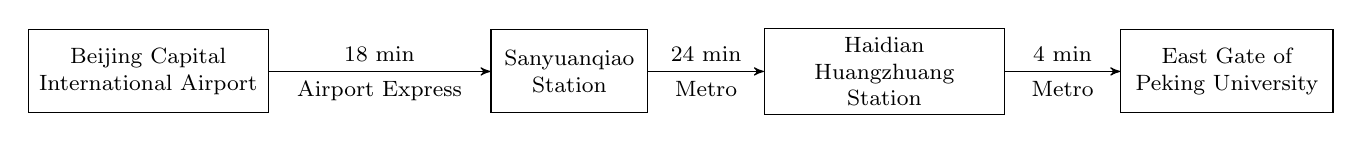
\begin{tikzpicture}[font=\footnotesize]
\node(cia)[shape=rectangle,draw,text width=8em,text centered, minimum height=3em] at (-6.85,0){Beijing Capital\\ International Airport};
\node(syq)[shape=rectangle,draw,text width=5em,text centered, minimum height=3em] at (-1.5,0){Sanyuanqiao Station};
\node(hhz)[shape=rectangle,draw,text width=8em,text centered, minimum height=3em] at (2.5,0){Haidian Huangzhuang Station};
\node(pku)[shape=rectangle,draw,text width=7em,text centered, minimum height=3em] at (6.85,0){East Gate of Peking University};
\draw[->,>=stealth'] (cia)--(syq) node[midway,above]{18 min} node[midway,below]{Airport Express};
\draw[->,>=stealth'] (syq)--(hhz) node[midway,above]{24 min} node[midway,below]{Metro};
\draw[->,>=stealth'] (hhz)--(pku) node[midway,above]{4 min} node[midway,below]{Metro};
\end{tikzpicture}


\newpage
\phantomsection
\addsec{Registration/Information Desk}\rhead{Registration/Information desk}
The registration desk at Room 104 in the Peking University Overseas Exchange Center, will be open from 8:30‐18:00 on Tuesday 17th October.

\phantomsection
\addsec{Instructions for Presenters}
\begin{itemize}
\item According to SPHERIC Workshop Presentation Style, each presenter will have 13 minutes strictly to present their work, followed by the successive presenter.  After all the presentations in a specific session, all the presenters will be asked to stand in front of the conference room and answer possible questions in a Group.
\item There is no need to explain the very basics of SPH to an SPH specialist audience, and please emphasize what is new and novel in method or application.
\end{itemize}

\phantomsection
\addsec{SPH Training Day}

Supplementary to the workshop, an SPH training day will be offered on 17 October 2017. The training is most suitable for researchers who are familiar with the principles of SPH but are beginning their work in the field. More experienced SPH developers and users may find that the training day is a useful opportunity for sharing insights and ideas. The SPH training day will also take place at the Peking University.

\phantomsection
\addsec{Other Tips}
\textbf{Free wifi connection}: TBD, EDUROAM is also available.

\textbf{Name tags}: Name tags are required for entry to all conference events. Please wear them at all times.


\newgeometry{left=0.8in,right=0.8in,top=0.8in,bottom=0.8in}
\begin{landscape}
\pagestyle{plain}
\fancyhead{}
\phantomsection
\addsec{Beijing Subway Map}
\begin{center}
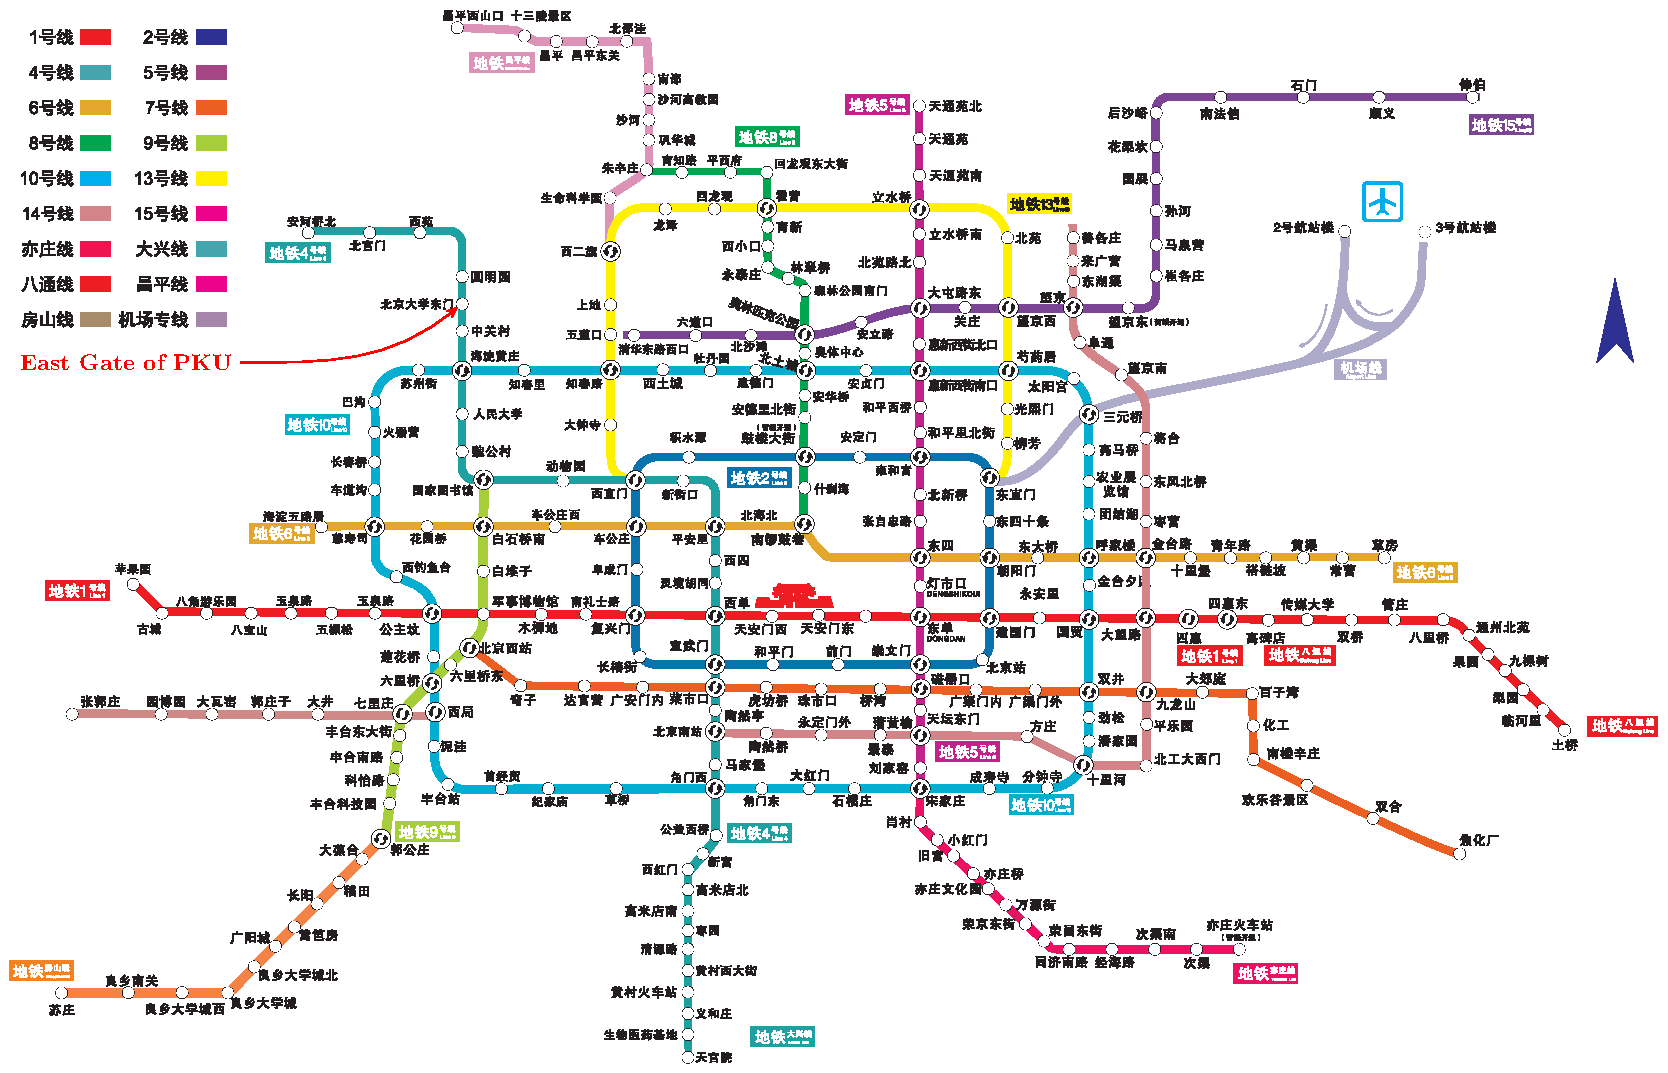
\includegraphics[height=0.925\textheight]{subway.pdf}
\end{center}
\end{landscape}

\begin{landscape}
\pagestyle{plain}
\fancyhead{}
\phantomsection
\addsec{Map of Peking University Campus}
\begin{center}
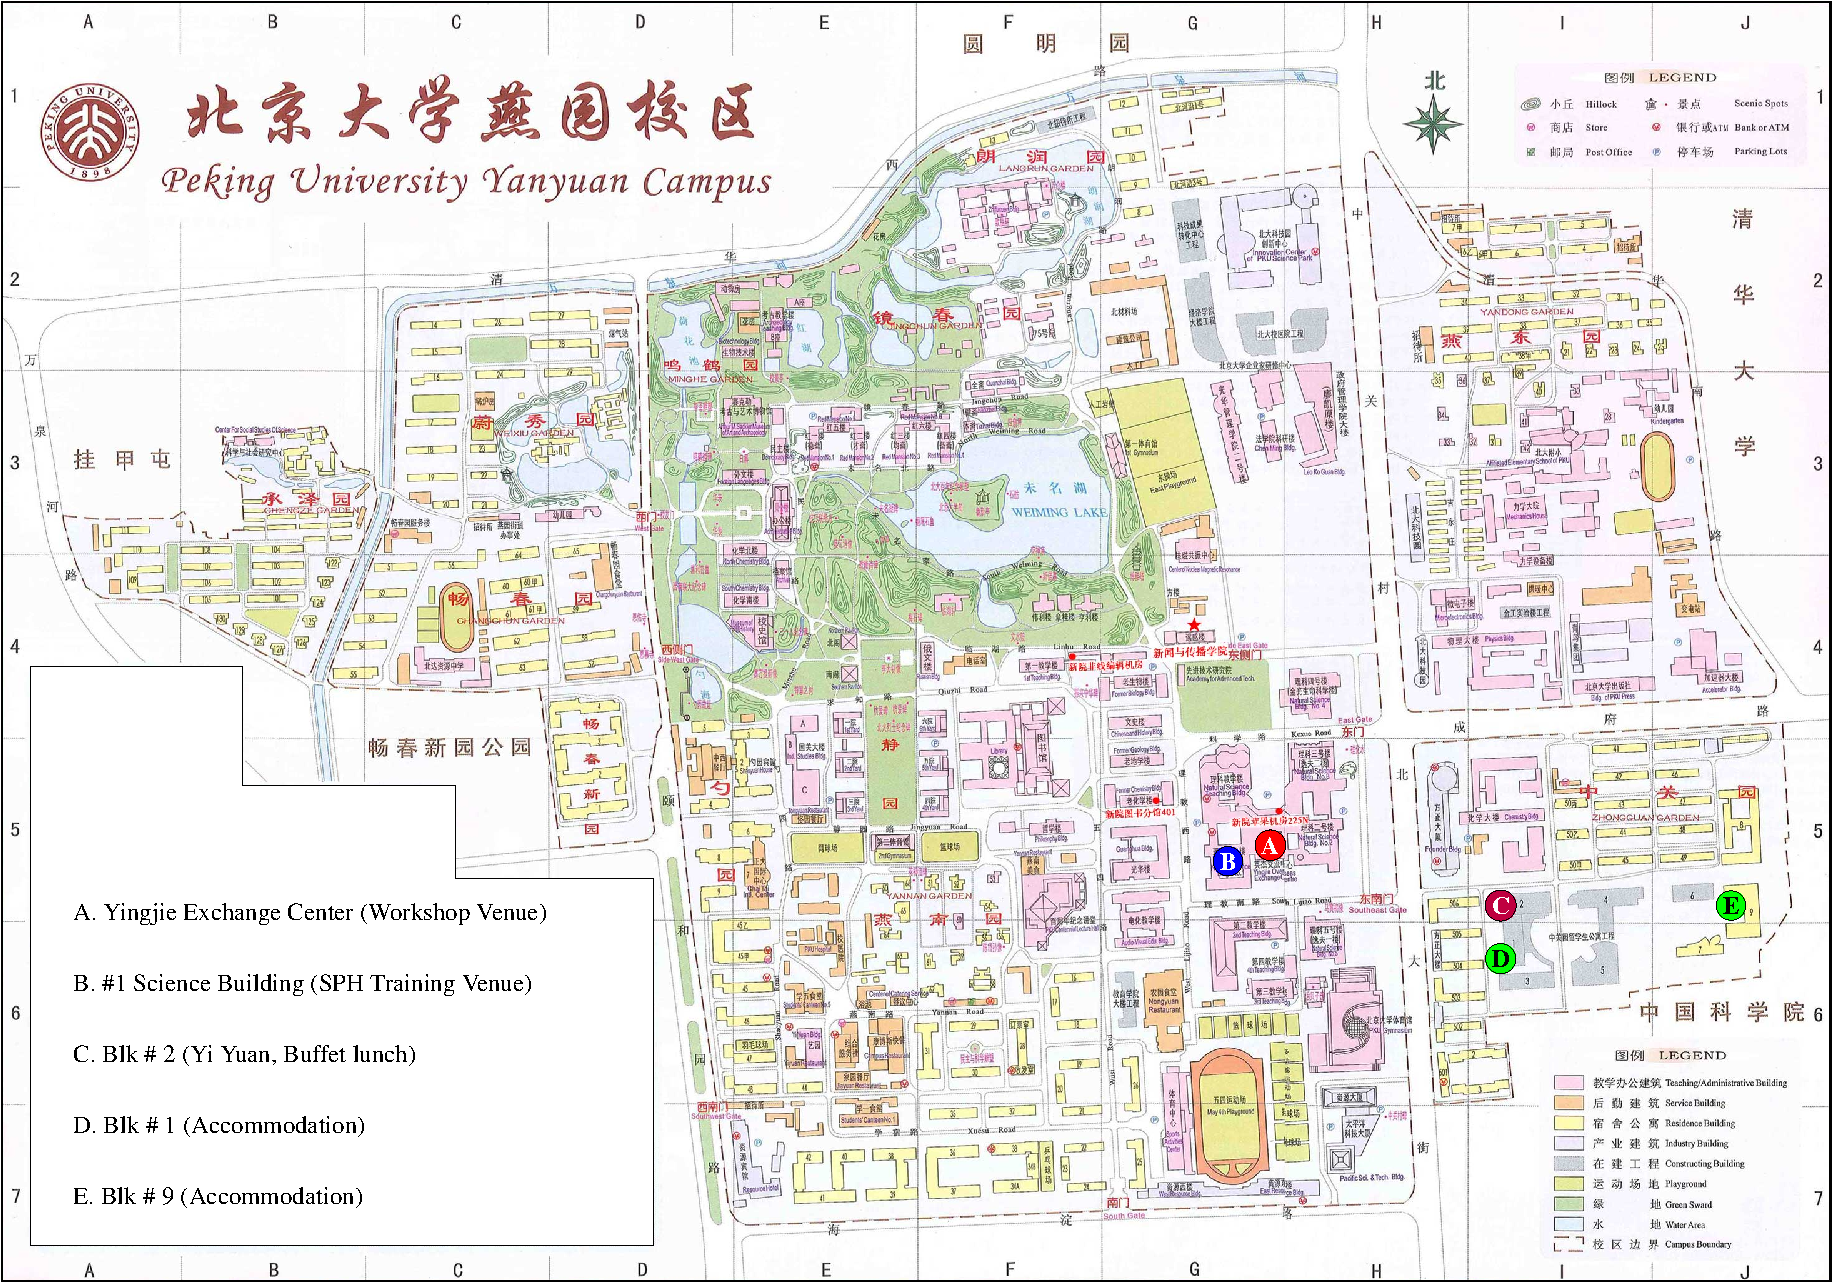
\includegraphics[height=0.925\textheight]{PKU.pdf}
\end{center}
\end{landscape}

\newgeometry{left=0.8in,right=0.8in,top=1in,bottom=0.7in}
\newpage
\lhead{SPHERIC Beijing 2017} \rhead{Floor Plan of Yingjie Exchange Center}
\chead{Workshop Details}
\phantomsection
\addsec{Floor Plan of Yingjie Exchange Center, Peking University}
\begin{center}
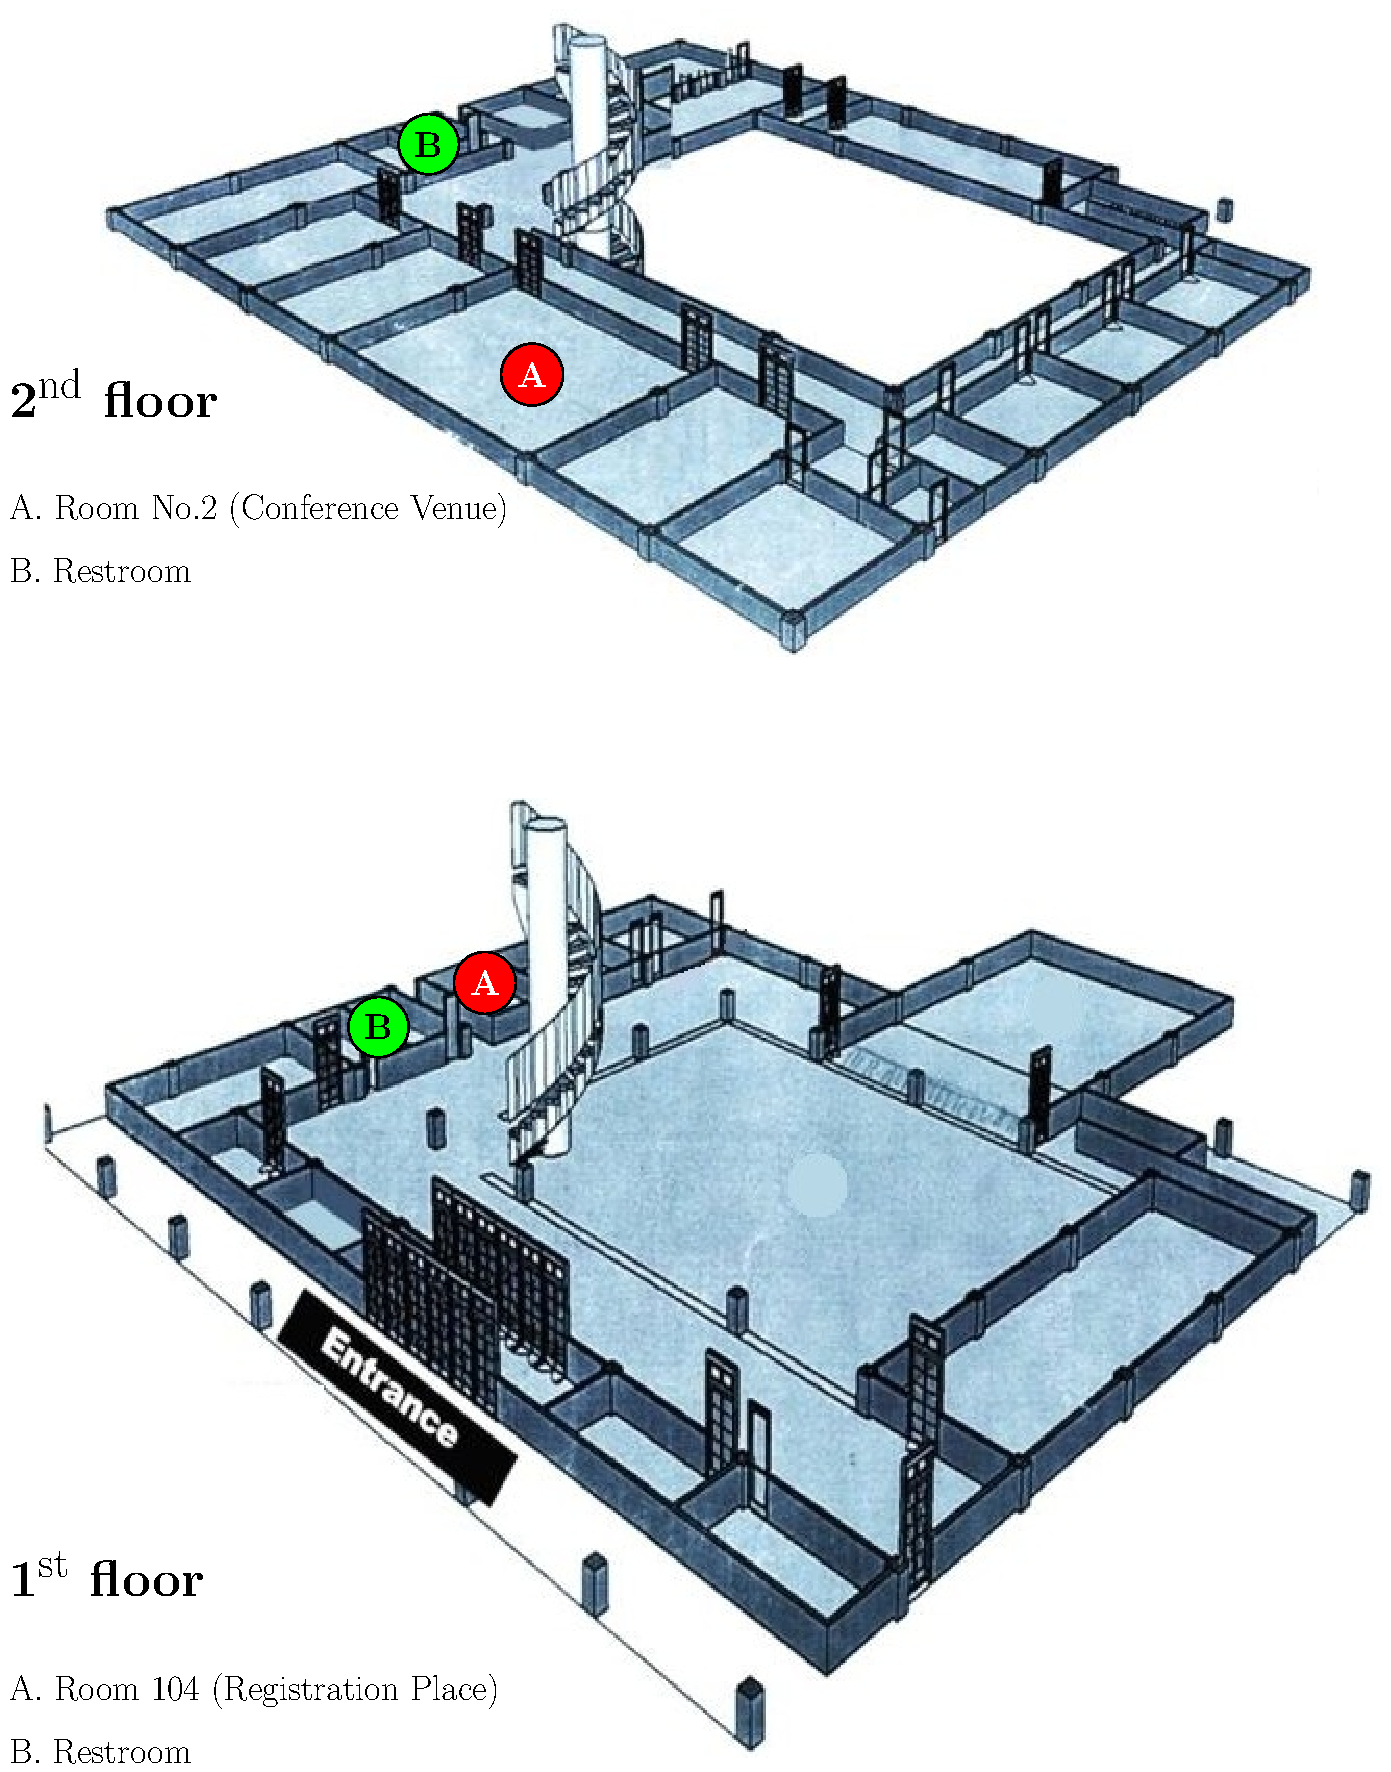
\includegraphics[width=\textwidth]{YJ.pdf}
\end{center}













%\chapter*{Committees}\rhead{Committees}
%\addstarredchapter{Committees}
%\chaptermark{Committees}
\addcontentsline{toc}{chapter}{Committees} \mtcaddchapter
\vspace{-5em}

\section*{Scientific Committee}\vspace{-1em}
%\addcontentsline{toc}{section}{Scientific Committee} 
\begin{itemize}
\item Prof. David Le Touz\'e (Ecole Centrale de Nantes, France)
\item Dr. Damien Violeau (Electricit\'e de France, France)
\item Dr. Nathan Quinlan (National Univ. of Ireland, Ireland)
\item Dr. Ben Rogers (University of Manchester, UK)
\item Prof. Stefano Sibilla (University of Pavia, Italy)
\item Dr. Jean-Christophe Marongiu (ANDRITZ Hydro, France)
\item Dr. Alex Crespo (Universidade de Vigo, Spain)
\item Dr. Andrea Colagrossi (INSEAN, Italy)
\item Dr. Xiangyu Hu (Technical University of Munich, Germany)
\item Prof. Rade Vignjevic (Brunel University of London, UK)
\item Prof. Thomas Rung (Technical University of Hamburg-Harburg, Germany)
\item Dr. Antonio Souto-Iglesias (Technical University of Madrid, Spain)
\item Dr. Renato Vacondio (University of Parma, Italy)
\item Dr. Matthieu De Leffe (Nextflow Software, France)
\item Prof. Moncho G\'omez-Gesteira (Universidade de Vigo, Spain)
\item Dr. Abbas Khayyer (University of Kyoto, Japan)
\item Prof. Walter Dehnen (University of Leicester, UK)
\item Dr. Raj Das (University of Auckland, New Zealand)
\item Prof. Robert A. Dalrymple (Johns Hopkins University , USA)
\item Prof. Alexis H\'erault (Conservatoire National des Arts et M\'etiers, France)
\item Prof. Joe Monaghan (Monash University, Australia)
\item Prof. Peter Eberhard (University of Stuttgart, Germany)
\item Prof. Moubin Liu (Peking University, China)
\item Dr Mehmet Yildiz (Sabanci University, Turkey)
\end{itemize}



\section*{Organizing Committee}
%\addcontentsline{toc}{section}{Organizing Committee} 
\subsection*{Chair}\vspace{-1em}
\begin{itemize}
\item Prof.   M. B. Liu, Peking University
\end{itemize}

\subsection*{Co-Chairs}\vspace{-1em}
\begin{itemize}
\item Prof.   H. F. Qiang, Xi'an Hi-Tech Institute, China
\item Prof.   A. M. Zhang, Harbin Engineering University, China
\item Prof.   L. Zou, Dalian University of Technology, China
\item Prof.   D. A. Hu, Hunan University, China
\item Prof.   F. Xu, Northwestern Polytechnical University, China
\item Prof.   Z. R. Li, Wenzhou University, China
\end{itemize}




\newgeometry{left=0.8in,right=0.8in,top=0in,bottom=0.7in}

\chapter*{Program}\chead{Program}
%\addstarredchapter{Workshop Program}
%\chaptermark{Workshop Program}
\addcontentsline{toc}{chapter}{Program} \mtcaddchapter
\vspace{-5em}

%\newpage
\phantomsection
\addsec{Program Overview}\rhead{Program Overview}
%\section*{Program Overview}
%\addcontentsline{toc}{section}{Program Overview}\mtcaddchapter
\setslotsize{3.375cm}{0.3cm}
\setslotcount{4}{66}
\setbottomspace{0pt}
\settextframe{3pt}

% Define event types
\defineevent{keynote}{0.0} {0.28}{1.0} {1.0}{1.0}{1.0}
\defineevent{session}{0.0} {0.6}{1.0} {1.0}{1.0}{1.0}
\defineevent{dining}    {1.0} {0.4} {0.2} {1.0}{1.0}{1.0}
\defineevent{coffee}    {1.0} {0.4} {0.8} {1.0}{1.0}{1.0}
\defineevent{registration} {1.0} {0.4} {0.2} {1.0}{1.0}{1.0}
\defineevent{training}   {0.21}{0.5} {0.16}{1.0}{1.0}{1.0} 
\defineevent{opening}      {0.8} {0.2} {0.2} {1.0}{1.0}{1.0}

% Start the time table
%\noindent\printheading{PROGRAM OVERVIEW}
%\vspace{-0.5em}
\begin{timetable}
  \hours{8}{10}{1}
  \englishdays{2}
  \event 1 {0900} {1030} {Training Session 1}                  {9:00}        {10:30}     {training}
  \event 1 {1030} {1050} {\vspace{0.1em}Coffee: {\scriptsize 10:30--10:50}}        {}     {} {coffee}
  \event 1 {1050} {1220} {Training Session 2}               {10:50}         {12:20}   {training}
  \event 1 {1220} {1315} {Lunch}                  {12:20}        {13:15}     {dining}
  \event 1 {1315} {1345} {Training Session 3}                       {13:15}         {13:45}   {training}
  \event 1 {1345} {1415} {Training Session 4}                  {13:45}        {14:15}     {training}
  \event 1 {1415} {1530} {Training Session 5I}                       {14:15}         {15:30}   {training}
  \event 1 {1530} {1550} {\vspace{0.1em}Coffee: {\scriptsize 15:30--15:45}}        {}     {} {coffee}
  \event 1 {1550} {1730} {Training Session 5II}                       {15:45}         {17:30}   {training}
  \event 1 {1730} {1830} {Dinner}                  {17:30}        {}     {dining}
  
  \event 2 {0800} {0845} {Registration}               {8:00}      {8:45}     {registration}
  \event 2 {0845} {0915} {Opening}        {8:45}     {9:15} {opening}
  \event 2 {0915} {1010} {Keynote 1}                    {9:15}         {10:10} {keynote}
  \event 2 {1010} {1100} {Session 1}               {10:10}      {11:00}     {session}
  \event 2 {1100} {1120} {\vspace{0.1em}Coffee: {\scriptsize 11:00--11:20}}        {}     {} {coffee}
  \event 2 {1120} {1225} {Session 2}               {11:20}      {12:25}     {session}
  \event 2 {1225} {1400} {Lunch}                  {12:25}        {14:00}     {dining}
  \event 2 {1400} {1505} {Session 3}               {14:00}      {15:05}     {session}
  \event 2 {1505} {1610} {Session 4}               {15:05}      {16:10}     {session}
  \event 2 {1610} {1630} {\vspace{0.1em}Coffee: {\scriptsize 16:10--16:30}}        {}     {} {coffee}
  \event 2 {1630} {1735} {Session 5}               {16:30}      {17:35}     {session}
  \event 2 {1735} {1830} {Dinner}                  {17:35}        {}     {dining}
  
  \event 3 {0900} {0955} {Keynote 2}                    {9:00}         {9:55} {keynote}
  \event 3 {0955} {1100} {Session 6}               {9:55}      {11:00}     {session}
  \event 3 {1100} {1120} {\vspace{0.1em}Coffee: {\scriptsize 11:00--11:20}}        {}     {} {coffee}
  \event 3 {1120} {1210} {Session 7}               {11:20}      {12:10}     {session}
  \event 3 {1210} {1400} {Lunch}                  {12:10}        {14:00}     {dining}
  \event 3 {1400} {1505} {Session 8}               {14:00}      {15:05}     {session}
  \event 3 {1505} {1525} {\vspace{0.1em}Coffee: {\scriptsize 15:05--15:25}}        {}     {} {coffee}
  \event 3 {1525} {1630} {Session 9}               {15:25}      {16:30}     {session}
  \event 3 {1630} {1700} {Take Bus To Yu Xian Du}                  {}        {\hspace{-2em}16:30--17:00}     {dining}
  \event 3 {1700} {1800} {Visit YXD Food Museum}                  {17:00}        {18:00}     {dining}
  \event 3 {1800} {1900} {Banquet \& Award}                  {18:00}        {21:00}     {opening}
  
  \event 4 {0900} {1005} {Session 10}               {9:00}      {10:05}     {session}
  \event 4 {1005} {1110} {Session 11}               {10:05}      {11:10}     {session}
  \event 4 {1110} {1130} {\vspace{0.1em}Coffee: {\scriptsize 11:10--11:30}}        {}     {} {coffee}
  \event 4 {1130} {1235} {Session 12}               {11:30}      {12:35}     {session}
  
  \event 4 {1235} {1400} {Lunch}                  {12:35}        {14:00}     {dining}
  \event 4 {1400} {1505} {Session 13}               {14:00}      {15:05}     {session}
  \event 4 {1505} {1610} {Session 14}               {15:05}      {16:10}     {session}
  \event 4 {1610} {1630} {\vspace{0.1em}Coffee: {\scriptsize 16:10--16:30}}        {}     {} {coffee}
  \event 4 {1630} {1720} {Session 15}               {16:30}      {17:20}     {session}
  \event 4 {1720} {1830} {Dinner}                  {17:20}        {}     {dining}
\end{timetable}

\newgeometry{left=0.8in,right=0.8in,top=1in,bottom=0.7in}


\newpage
%\begin{landscape}
\renewcommand{\arraystretch}{2}
\phantomsection
\addsec{SPH Training Day Program}\rhead{SPH Training Day Program}
%\section*{SPH Training Day Program}
%\addcontentsline{toc}{section}{SPH Training Day Program}\mtcaddchapter

\subsection*{Venue: Room 1338W, Level 3, \#1 Science Blk, Peking University}
\subsection*{地点:北京大学理科一号楼三层1338W房间(计算机中心8号机房)}

\newcolumntype{M}[1]{>{\centering\arraybackslash}m{#1}}
\newcolumntype{N}[1]{>{\arraybackslash}m{#1}}
\begin{tabularx}{\textwidth}{l|X|N{11em}}
%\begin{tabular}{|c|c|c|}
\hlinewd{1.5pt}
\textbf{Training day} & \textbf{17 October (Tuesday)} & \tabularnewline
\hlinewd{1pt}  
\hphantom{0}9:00-10:30 & Training Session 1: Theory and Application of SPH - Part 1: An Introduction
to Multi-Phase Modelling in SPH & Dr. Xiangyu Hu\tabularnewline
\hline 
10:30-10:50 & Coffee & \tabularnewline
\hline 
10:50-12:20 & Training Session 2: Advanced SPH/CG(Coarse-Grained) modelling for
biomechanics and biomedical systems  & Prof. Y. T. Gu\tabularnewline
\hline 
12:20-13:15 & Lunch & Box lunch\tabularnewline
\hline 
13:15-13:45 & Training Session 3: Simulation with DualSPHysics & Dr. Ben Rogers\tabularnewline
\hline 
13:45-14:15 & Training Session 4: Pre- and Post-Processing (Visualisation) with
DualSPHysics & Dr Jose Dominguez\tabularnewline
\hline 
14:15-15:30 & Training Session 5: Practical hands-on session with DualSPHysics I & \multirow{3}{*}{\shortstack[l]{Dr. Ben Rogers,\\ \\ \\ Dr. Jose Dominguez,\\ \\ \\ Dr. Jose González-Cao,\\ \\ \\ Mr. Feng Zhang}}\tabularnewline
\cline{1-2} 
15:30-15:45 & Coffee & \tabularnewline
\cline{1-2} 
15:45-17:30 & Training Session 5: Practical hands-on session with DualSPHysics II & \tabularnewline
\hline 
17:30\hphantom{-16:30} & Dinner & @PKU canteen with card\tabularnewline
\hlinewd{1.5pt}
\end{tabularx}

\vspace{2em}
\begin{itemize}
\item Full day registration (8:30AM to 18:00PM) at Room 104 in the Peking University Overseas Exchange Center\\
10月17日全天上午8:30 到 下午18:00亦在北京大学英杰交流中心104室注册
\end{itemize}
%\end{tabular}

%\end{landscape}


\newpage
\phantomsection
\addsec{SPHERIC Beijing 2017 Workshop Program}\rhead{Workshop Program}
%\section*{SPHERIC Beijing 2017 Workshop Program}
%\addcontentsline{toc}{section}{SPHERIC Beijing 2017 Workshop Program}\mtcaddchapter
\subsection*{Venue: Conference Room \#2, Peking University Overseas Exchange Centre}
\subsection*{地点:北京大学英杰交流中心第二会议室}


%\begin{tabular}{|c|l|l|l|}
\begin{tabularx}{\textwidth}{l|X|N{21em}|N{9em}}
\hlinewd{1.5pt}
\textbf{1st DAY} & \multicolumn{3}{l}{\textbf{18 October (Wednesday)}}\tabularnewline
\hlinewd{1pt}
08:00-08:45 & \multicolumn{3}{l}{Registration}\tabularnewline
\hline 
\multirow{2}{*}{08:45-09:15} & \multirow{2}{*}{Opening} & Speech by: B. Rogers & \multirow{2}{*}{Chair: M. B. Liu}\tabularnewline
 &  & Speech by: J. X. Wang, Vice Dean of CoE, PKU & \tabularnewline
\hline 
09:15-10:10 & \multicolumn{2}{p{\dimexpr0.475\linewidth+10\tabcolsep}|}{\hyperref[David]{Keynote 1: Smoothed particle hydrodynamics, fact checking: from theory to applications by Prof. David Le Touzé, Ecole Centrale de Nantes}} & Chair: J. X. Wang\tabularnewline
\hline 
\multirow{2}{*}{10:10-11:00} & \multicolumn{2}{l|}{\hyperref[1.1]{Session 1: Maritime and Naval Architecture Applications}} & Chair: A. Colagrossi \tabularnewline
\cline{2-4} 
 & \multicolumn{3}{p{\dimexpr0.825\linewidth+0\tabcolsep}}{
\vspace{-1.5em}
\begin{itemize}
\item[1.1] \hyperref[1.1]{``DualSPHysics: a numerical tool to simulate real breakwaters'' \underline{F. Zhang}$^\text{Student Prize}$, S. P. Shang, Alejandro Crespo, José Dominguez, Moncho Gomez-Gesteira, Corrado Altomare, Andrea Marzeddu}
\item[1.2] \hyperref[1.2]{``High speed water impacts of fat plates in different ditching configurations through a Riemann-ALE SPH model'' \underline{S. Marrone}, A. Colagrossi, M. De Leffe, L. Chiron, D. Le Touze}
%\item[1.2] \hyperref[1.2]{``Numerical simulation of green water using SPH method'' \underline{L. J. Wen}, Q. D. Feng}
\item[1.3] \hyperref[1.3]{``Application of improved SPH solid-wall boundary model in missile water exiting'' \underline{H. L. Zheng}, H. F. Qiang, F. Z. Chen, C. Shi}
\end{itemize}
}\tabularnewline
\hline 
 11:00-11:20 & \multicolumn{3}{l}{Coffee} \tabularnewline
\hline 
\multirow{2}{*}{11:00-12:25} & \multicolumn{2}{l|}{\hyperref[2.1]{Session 2: Multiple Continua and Multi-Phase Flows}} & Chair: X. Y. Hu \tabularnewline
\cline{2-4} 
 & \multicolumn{3}{p{\dimexpr0.825\linewidth+0\tabcolsep}}{
\vspace{-1.5em}
\begin{itemize}
\item[2.1] \hyperref[2.1]{``Multiphase Godunov-typed smoothed particle hydrodynamics method with approximate Riemann solvers'' \underline{Z. W. Cai}, Z. Zong, L. Zhou, Z. Chen, C. Tiao}
\item[2.2] \hyperref[2.2]{``A two-phase SPH model for sediment laden flows'' \underline{H. B. Shi}, X. P. Yu}
\item[2.3] \hyperref[2.3]{``Numerical simulation of water-entry problems using an improved multiphase SPH method'' \underline{H. Cheng}$^\text{Student Prize}$, A. M. Zhang, F. R. Ming}
\item[2.4] \hyperref[2.4]{``Stable sharp interface method for SPH'' \underline{M. Y. Zhang}}
\end{itemize}
}\tabularnewline
\hline 
12:25-14:00 & \multicolumn{3}{l}{Lunch (Buffet lunch @ ZhongGuanYuan Global Village PKU)} \tabularnewline
\hline 
\multirow{2}{*}{14:00-15:05} & \multicolumn{2}{l|}{\hyperref[3.1]{Session 3: Impacts with Fluids or Solids}} & Chair: X. H. Guo \tabularnewline
\cline{2-4} 
 & \multicolumn{3}{p{\dimexpr0.825\linewidth+0\tabcolsep}}{
\vspace{-1.5em}
\begin{itemize}
\item[3.1] \hyperref[3.1]{``Aircraft tire water spray simulation using SPH'' \underline{Y. K. Hu}, Y. F. Rong, D. X. Leng, F. Xu, X. Y. Gao, R. G. Cao, W. Ding, J. Lv}
\item[3.2] \hyperref[3.2]{``Numerical simulation of the damage of multi-floor buildings by conical projectile with SPH method'' H. F. Qiang, \underline{X. Y. Sun}, F. Z. Chen, G. X. Zhang }
\item[3.3] \hyperref[3.3]{``Corrected smoothed particle hydrodynamics for simulating failure progress of model-scale ice'' \underline{X. Zheng}, N. B. Zhang, Q. W. Ma}
\item[3.4] \hyperref[3.4]{``Numerical study of the mechanism of explosive/impact welding using an improved SPH method'' \underline{Z. L. Zhang}$^\text{Student Prize}$, M. B. Liu}
\end{itemize}
}\tabularnewline
\hline 
\multirow{2}{*}{15:05-16:10} & \multicolumn{2}{l|}{\hyperref[4.1]{Session 4: Free Surface and Moving Boundaries Applications}} & Chair: X. F. Yang \tabularnewline
\cline{2-4} 
 & \multicolumn{3}{p{\dimexpr0.825\linewidth+0\tabcolsep}}{
\vspace{-1.5em}
\begin{itemize}
\item[4.1] \hyperref[4.1]{``SPH numerical investigation of oscillating characteristics of hydraulic jumps at an abrupt drop'' Diana De Padova, Michele Mossa, \underline{Stefano Sibilla}}
\item[4.2] \hyperref[4.2]{``An SPH simulation of bubble cavity evolution on underwater movement'' \underline{J. R. Shao}, M. B. Liu}
\item[4.3] \hyperref[4.3]{``The $\delta$ALE-SPH model: an improved $\delta$-SPH scheme containing particle shifting and ALE formulation'' \underline{P. N. Sun}$^\text{Student Prize}$, A. M. Zhang, A. Colagrossi, S. Marrone, M. Antuono}
\item[4.4] \hyperref[4.4]{``SPH numerical simulation of lift-off by impact of sand particles on flat sand bed'' \underline{J. Zhao}, A. F. Jin, Maimtimin Geni, X. J. Ma}
\end{itemize}
}\tabularnewline
\hline 
 16:10-16:30 & \multicolumn{3}{l}{Coffee} \tabularnewline
\hline 
\multirow{2}{*}{16:30-17:35} & \multicolumn{2}{l|}{\hyperref[5.1]{Session 5: Geotechnical  Applications}} & Chair: J. S. Wu \tabularnewline
\cline{2-4} 
 & \multicolumn{3}{p{\dimexpr0.825\linewidth+0\tabcolsep}}{
\vspace{-1.5em}
\begin{itemize}
\item[5.1] \hyperref[5.1]{``A comparative study of SPH and MPM in modeling mixed-mode failure in rocks'' \underline{Sam Raymond}$^\text{Student Prize}$, Bruce Jones, John Williams}
\item[5.2] \hyperref[5.2]{``A SPH investigation of soil plastic behaviour with Mohr-Coulomb constitutive model'' \underline{S. H. Zhao}, Ha H. Bui, Vincent Lemiale, Giang D. Nguyen}
\item[5.3] \hyperref[5.3]{``A robust approach to model rock fracture with SPH'' \underline{Y. N. Wang}, Ha H. Bui, Giang D. Nguyen, P. G. Ranjith} 
\item[5.4] \hyperref[5.4]{``An elasto-plastic-$\mu$(I) SPH model for landslide induced debris flow'' \underline{W. T. Zhang}, Y. An, Q. Q. Liu}
\end{itemize}
}\tabularnewline
\hline 
17:35\hphantom{-16:30} & \multicolumn{3}{l}{\textbf{Dinner} @PKU canteen with card} \tabularnewline
\hlinewd{1.5pt}
\end{tabularx}
%\end{tabular}



\newpage




%\begin{tabular}{|c|l|l|l|}
\begin{tabularx}{\textwidth}{l|X|N{21em}|N{9em}}
\hlinewd{1.5pt}
\textbf{2nd DAY} & \multicolumn{3}{l}{\textbf{19 October (Thursday)}}\tabularnewline
\hlinewd{1pt}
09:00-09:55 & \multicolumn{2}{p{\dimexpr0.475\linewidth+10\tabcolsep}|}{\hyperref[Chen]{Keynote 2: An implicit gradient reproducing kernel particle method: theory and applications by Prof. J. S. Chen, University of California}} & Chair: P. Chen, Head, Division of Computational Mechanics , PKU\vspace{-2em}\tabularnewline
\hline 
\multirow{2}{*}{09:55-11:00} & \multicolumn{2}{l|}{\hyperref[6.1]{Session 6: Hydraulic Applications I}} & Chair: S. Marrone \tabularnewline
\cline{2-4} 
 & \multicolumn{3}{p{\dimexpr0.825\linewidth+0\tabcolsep}}{
\vspace{-1.5em}
\begin{itemize}
\item[6.1]\hyperref[6.1]{``Overview of SPH-ALE applications for hydraulic turbines in ANDRITZ Hydro'' Jean-Christophe Marongiu, Magdalena Neuhauser, \underline{Martin Rentschler}, Etienne Parkinson} 
\item[6.2]\hyperref[6.2]{``Numerical and experimental investigation of two porous wave - breaking structures'' W. Q. Hu, \underline{Q. Fan}$^\text{Student Prize}$, J. M. Zhan, W. H. Cai} 
\item[6.3]\hyperref[6.3]{``SPH for the interaction between tsunami wave and upright cylindrical groups'' \underline{J. J. Li}$^\text{Student Prize}$, L. Tian, Y. S. Yang, L. C. Qiu, Y. Han}
\item[6.4]\hyperref[6.4]{``Hydrodynamics characteristics of land hinged oscillating wave surge converter with SPH method''
D. H. Zhang, \underline{Y. X. Shi}, C. Huang, Y. L. Si, B. Huang, and W. Li }
\end{itemize}
}\tabularnewline
\hline 
 11:00-11:20 & \multicolumn{3}{l}{Coffee} \tabularnewline
\hline 
\multirow{2}{*}{11:20-12:10} & \multicolumn{2}{l|}{\hyperref[7.1]{Session 7: Adaptivity (variable resolution)}} & Chair: L. C. Qiu \tabularnewline
\cline{2-4} 
 & \multicolumn{3}{p{\dimexpr0.825\linewidth+0\tabcolsep}}{
\vspace{-1.5em}
\begin{itemize}
\item[7.1]\hyperref[7.1]{``The study on SPH method with space variable smoothing length and its applications to multi-phase flow'' \underline{W. K. Shi}$^\text{Student Prize}$, Y. M. Shen , J. Q. Chen}
\item[7.2]\hyperref[7.2]{``A dynamic refinement strategy in SPH for simulating the water entry of an elastomer'' \underline{L. Wang}, F. Xu, Y. Yang}
\item[7.3]\hyperref[7.3]{``Adaptive particle splitting in the finite volume particle method'' \underline{Nathan J. Quinlan}}
\end{itemize}
}\tabularnewline
\hline 
12:10-14:00 & \multicolumn{3}{l}{Lunch @PKU canteen with card} \tabularnewline
\hline 
\multirow{2}{*}{14:00-15:05} & \multicolumn{2}{l|}{\hyperref[8.1]{Session 8: New applications of SPH}} & Chair: David Le Touzé \tabularnewline
\cline{2-4} 
 & \multicolumn{3}{p{\dimexpr0.825\linewidth+0\tabcolsep}}{
\vspace{-1.5em}
\begin{itemize}
\item[8.1]\hyperref[8.1]{`` Modeling the melting process of quartz glass using SPH method'' \underline{Z. Y. Liu}$^\text{Student Prize}$, Q. L. Ma, H. S. Fang} 
\item[8.2]\hyperref[8.2]{``Study on dynamic behaviors of liquid-filled flexible multibody systems under the low-gravity environment'' \underline{W. Z. Kong}, Q. Tian}
\item[8.3]\hyperref[8.3]{``A SPH model for the root system of plants'' \underline{Matthias Mimault}, Lionel Dupuy, Mariya Ptashnyk}
\item[8.4]\hyperref[8.4]{``SPH simulation of drop impact on a hot wall with vaporization effects'' \underline{X. F. Yang}, S. C. Kong, M. B. Liu}
\end{itemize}
}\tabularnewline
\hline 
 15:05-15:25 & \multicolumn{3}{l}{Coffee} \tabularnewline
\hline 
\multirow{2}{*}{15:25-16:30} & \multicolumn{2}{l|}{\hyperref[9.1]{Session 9: High-Performance Computing}} & Chair: B. Rogers \tabularnewline
\cline{2-4} 
 & \multicolumn{3}{p{\dimexpr0.825\linewidth+0\tabcolsep}}{
\vspace{-1.5em}
\begin{itemize}
\item[9.1] \hyperref[9.1]{``Developing an extensible, portable, scalable toolkit for massively parallel incompressible smoothed particle hydrodynamics (ISPH)'' \underline{X. H. Guo}, Benedict D. Rogers, Steven Lind, Peter K. Stansby}
\item[9.2] \hyperref[9.2]{``Three-dimensional sloshing simulations by using GPU-based MPS method'' \underline{X. Chen}, X. Wen, D. C. Wan}
\item[9.3] \hyperref[9.3]{``GPU-based SPH modeling of flood with floating bodies in urban layouts including underground spaces'' \underline{J. S. Wu}, N. Li, W. Y. Liu, H. Zhang}
\item[9.4] ``Improve the effectively of computational fluid dynamics work based on supercomputing cloud'' \underline{N. Qiao} % no abstract
\end{itemize}
}\tabularnewline
\hline 
16:30-17:00 & \multicolumn{3}{l}{Take Bus To Yu Xian Du (YXD)} \tabularnewline
\hline 
17:00-18:00 & \multicolumn{3}{l}{Visit the YXD Food Museum} \tabularnewline
\hline 
18:00-21:00 & \multicolumn{3}{l}{Conference Banquet \& Award} \tabularnewline
\hlinewd{1.5pt} 
\end{tabularx}
%\end{tabular}



\newpage




%\begin{tabular}{|c|l|l|l|}
\begin{tabularx}{\textwidth}{l|X|N{21em}|N{9em}}
\hlinewd{1.5pt}
\textbf{3rd DAY} & \multicolumn{3}{l}{\textbf{20 October (Friday)}}\tabularnewline
\hlinewd{1pt}
\multirow{2}{*}{09:00-10:05} & \multicolumn{2}{l|}{\hyperref[10.1]{Session 10: Numerical Aspects of SPH}} & Chair: N. Quinlan \tabularnewline
\cline{2-4} 
 & \multicolumn{3}{p{\dimexpr0.825\linewidth+0\tabcolsep}}{
\vspace{-1.5em}
\begin{itemize}
\item[10.1]\hyperref[10.1]{``SPH energy balance during the generation and propagation of gravity waves'' \underline{Domenico Davide Meringolo}, Y. Liu, A. Colagrossi}
\item[10.2]\hyperref[10.2]{``Water hammer analysis using SPH in density summation form'' \underline{D. Q. Hou}, C. Y. Huang, M. L. Wang, H. F. Duan}
\item[10.3]\hyperref[10.3]{``Particle trajectory calculation in SPH'' \underline{J. Y. Shen}, W. H. Lu, D. Q. Hou, Arris S. Tijsseling}
\item[10.4]\hyperref[10.4]{``Simulating shock waves with corrective smoothed particle method (CSPM)'' \underline{C. Y. Huang}, J. Deng, D. Q. Hou, Arris S. Tijsseling}
\end{itemize}
}\tabularnewline
\hline 
\multirow{2}{*}{10:05-11:10} & \multicolumn{2}{l|}{\hyperref[11.1]{Session 11: Fluid Structure Interaction}} & Chair: M. De Leffe \tabularnewline
\cline{2-4} 
 & \multicolumn{3}{p{\dimexpr0.825\linewidth+0\tabcolsep}}{
\vspace{-1.5em}
\begin{itemize}
\item[11.1]\hyperref[11.1]{``SPH modeling of fluid-structure interaction (FSI)''  L. H. Han, \underline{X. Y. Hu}}
\item[11.2]\hyperref[11.2]{``Numerical modeling of 2D complex movement patterns to FSI problems using smoothed particle hydrodynamics'' \underline{C. Zhuang}, D. A. Hu, T. Long, G. Yang}
\item[11.3]\hyperref[11.3]{``Implement of the MPS-FEM coupled method for the FSI simulation of the 3-D dam-break problem'' \underline{Y. L. Zhang}, D. C. Wan}
\item[11.4]\hyperref[11.4]{``A new numerical method for SPH fluid-solid coupling simulation and its preliminary verification'' \underline{X. J. Ma}, Geni Mamtimin, A. F. Jin}
\end{itemize}
}\tabularnewline
\hline 
11:10-11:30 & \multicolumn{3}{l}{Coffee} \tabularnewline
\hline 
\multirow{2}{*}{11:30-12:35} & \multicolumn{2}{l|}{\hyperref[12.1]{Session 12: Modelling of Incompressible Flows}} & Chair: A. M. Zhang \tabularnewline
\cline{2-4} 
 & \multicolumn{3}{p{\dimexpr0.825\linewidth+0\tabcolsep}}{
\vspace{-1.5em}
\begin{itemize}
\item[12.1]\hyperref[12.1]{``An enhanced ISPH-SPH coupled method for incompressible fluid-elastic structure interactions'' Abbas Khayyer, Hitoshi Gotoh, \underline{Yuma Shimizu}, Hosein Falahaty}
\item[12.2]\hyperref[12.2]{``Interaction between solitary wave and flexible plate based on MPS-FEM coupled method'' \underline{C. P. Rao}, D. C. Wan}
\item[12.3]\hyperref[12.3]{``Modeling of single film bubble and numerical study of the plateau structure in foam system'' \underline{Z. G. Sun}, N. Ni, Y. J. Sun, G. Xi} 
\item[12.4]\hyperref[12.4]{``Numerical simulation of Rayleigh-Taylor instability by MPS multiphase method''  \underline{X. Wen}, D. C. Wan}
\end{itemize}
}\tabularnewline
\hline 
12:35-14:00 & \multicolumn{3}{l}{Lunch (Buffet lunch @ ZhongGuanYuan Global Village PKU)} \tabularnewline
\hline 
\multirow{2}{*}{14:00-15:05} & \multicolumn{2}{p{\dimexpr0.6\linewidth+0\tabcolsep}|}{\hyperref[13.1]{Session 13: Alternative Formulations and Particle-Based Simulation Techniques}} & Chair: M. B. Liu \tabularnewline
\cline{2-4} 
 & \multicolumn{3}{p{\dimexpr0.825\linewidth+0\tabcolsep}}{
\vspace{-1.5em}
\begin{itemize}
\item[13.1] \hyperref[13.1]{``Numerical simulation of particle collision and breakup behavior by SDPH-FVM coupling method'' H. F. Qiang, \underline{F. Z. Chen}}
\item[13.2] \hyperref[13.2]{``A physics evoked meshfree method'' Z. B. Ma, \underline{Y. Z. Zhao}}
\item[13.3] \hyperref[13.3]{``Suppression of non-physical voids in the finite volume particle method'' Mohsen H. Moghimi, \underline{Nathan J. Quinlan}}
\item[13.4] \hyperref[13.4]{``The Hermit-type RRKPM for piezoelectric materials'' \underline{J. C. Ma}, G. F. Wei}
\end{itemize}
}\tabularnewline
\hline 
\multirow{2}{*}{15:05-16:10} & \multicolumn{2}{l|}{\hyperref[14.1]{Session 14: Other applications of SPH}} & Chair: Stefano Sibilla \tabularnewline
\cline{2-4} 
 & \multicolumn{3}{p{\dimexpr0.825\linewidth+0\tabcolsep}}{
\vspace{-1.5em}
\begin{itemize}
\item[14.1] \hyperref[14.1]{``A development of a SPH model for simulation of abrasive-water-jet impacting on a metallic surface'' \underline{X. W. Dong}, Z. L. Li, J. L. Liu}
\item[14.2] \hyperref[14.2]{``SPH simulation of Couette flow with sinusoidally moving solid boundary'' \underline{H. Q. Li}, H. T. Liu, J. Z. Chang}
\item[14.3] \hyperref[14.3]{``Application of particle-based computational acoustics to sound propagation and scattering'' \underline{Y. O. Zhang}}
\item[14.4] \hyperref[14.4]{``Image processing with the SPH method'' \underline{C. Y. Huang}, W. H. Lu, D. Q. Hou, X. Cheng}
\end{itemize}
}\tabularnewline
\hline 
16:10-16:30 & \multicolumn{3}{l}{Coffee} \tabularnewline
\hline 
\multirow{2}{*}{16:30-17:20} & \multicolumn{2}{l|}{\hyperref[15.1]{Session 15: Hydraulic Applications II}} & Chair: M. Rentschler \tabularnewline
\cline{2-4} 
 & \multicolumn{3}{p{\dimexpr0.825\linewidth+0\tabcolsep}}{
\vspace{-1.5em}
\begin{itemize}
\item[15.1] \hyperref[15.1]{``Analysis of the hydrological safety of dams using numerical tools: Iber and DualSPHysics'' \underline{J. González-Cao}, O. García-Feal, A. J. C. Crespo, J. M. Domínguez, M. Gómez-Gesteira} 
\item[15.2] \hyperref[15.2]{``Construction of two-dimensional SPH numerical wave tank'' \underline{J. Y. Wang}, F. Xu, Y. Yang}
\item[15.3] \hyperref[15.3]{``An SPH numerical wave-current tank'' \underline{M. He}, H. S. Wang, X. F. Gao, W. H. Xu, Y. Shi}
\end{itemize}
}\tabularnewline
\hline 
17:20 & \multicolumn{3}{l}{Dinner @PKU canteen with card} \tabularnewline
\hlinewd{1.5pt} 
\end{tabularx}
%\end{tabular}

\chapter*{Abstracts}\chead{Abstracts}\rhead{Contents}
\addstarredchapter{Abstracts}
\chaptermark{Abstracts}

\vspace{-5em}
\minitoc \mtcskip \minilof


%\addcontentsline{toc}{chapter}{Abstracts} \mtcaddchapter


\newpage

\renewcommand{\thesection}{Session \arabic{section}}
\renewcommand{\thesubsection}{\arabic{section}.\arabic{subsection}}
%\section{Session 1: Maritime and Naval Architecture Applications}
%1.1: 22
%1.2: 32
%1.3: 36

\rhead{Session 1}
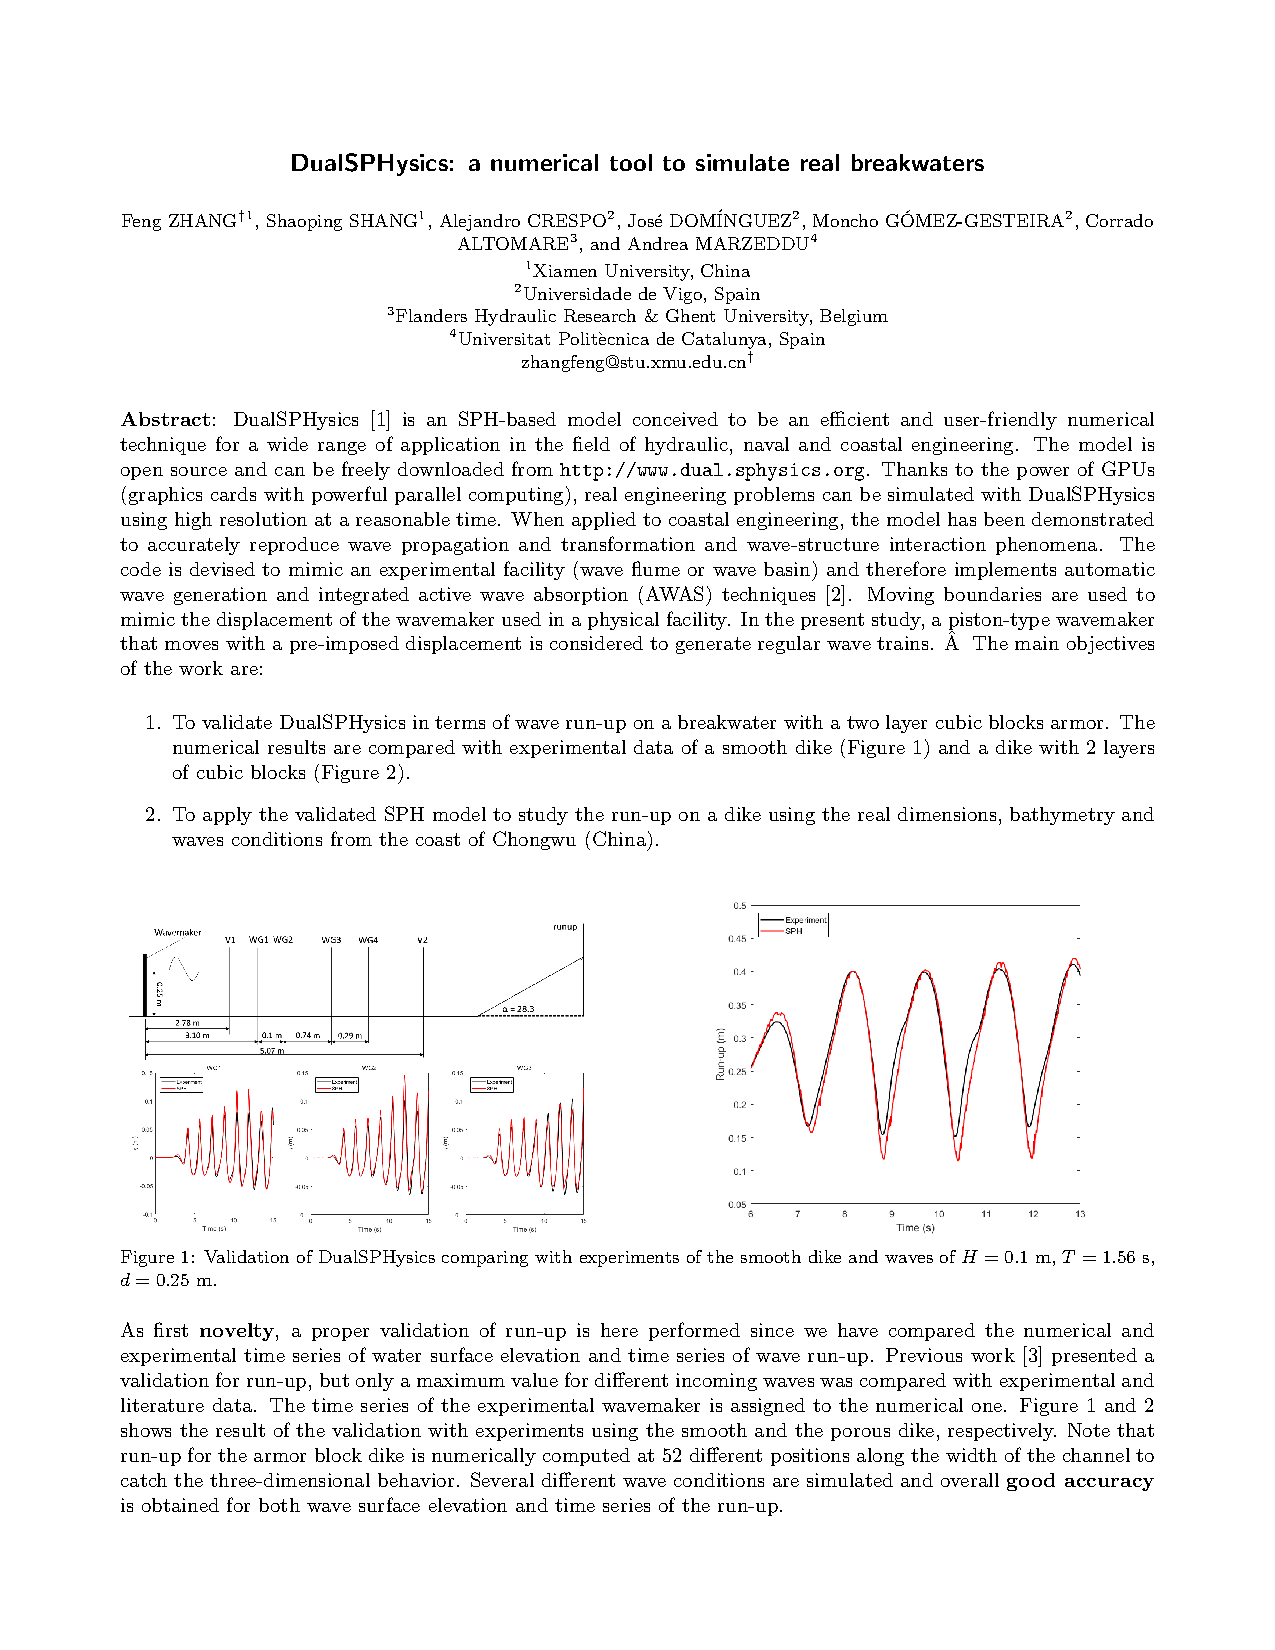
\includepdf[pages=-,pagecommand={\pagestyle{fancy}\label{1.1}},addtotoc={
     1,section,1,{~~~~~~~~Maritime and Naval Architecture Applications},p1,   
     1,subsection,1,DualSPHysics: a numerical tool to simulate real breakwaters,p1}]{abstract/pdfs/22.pdf}
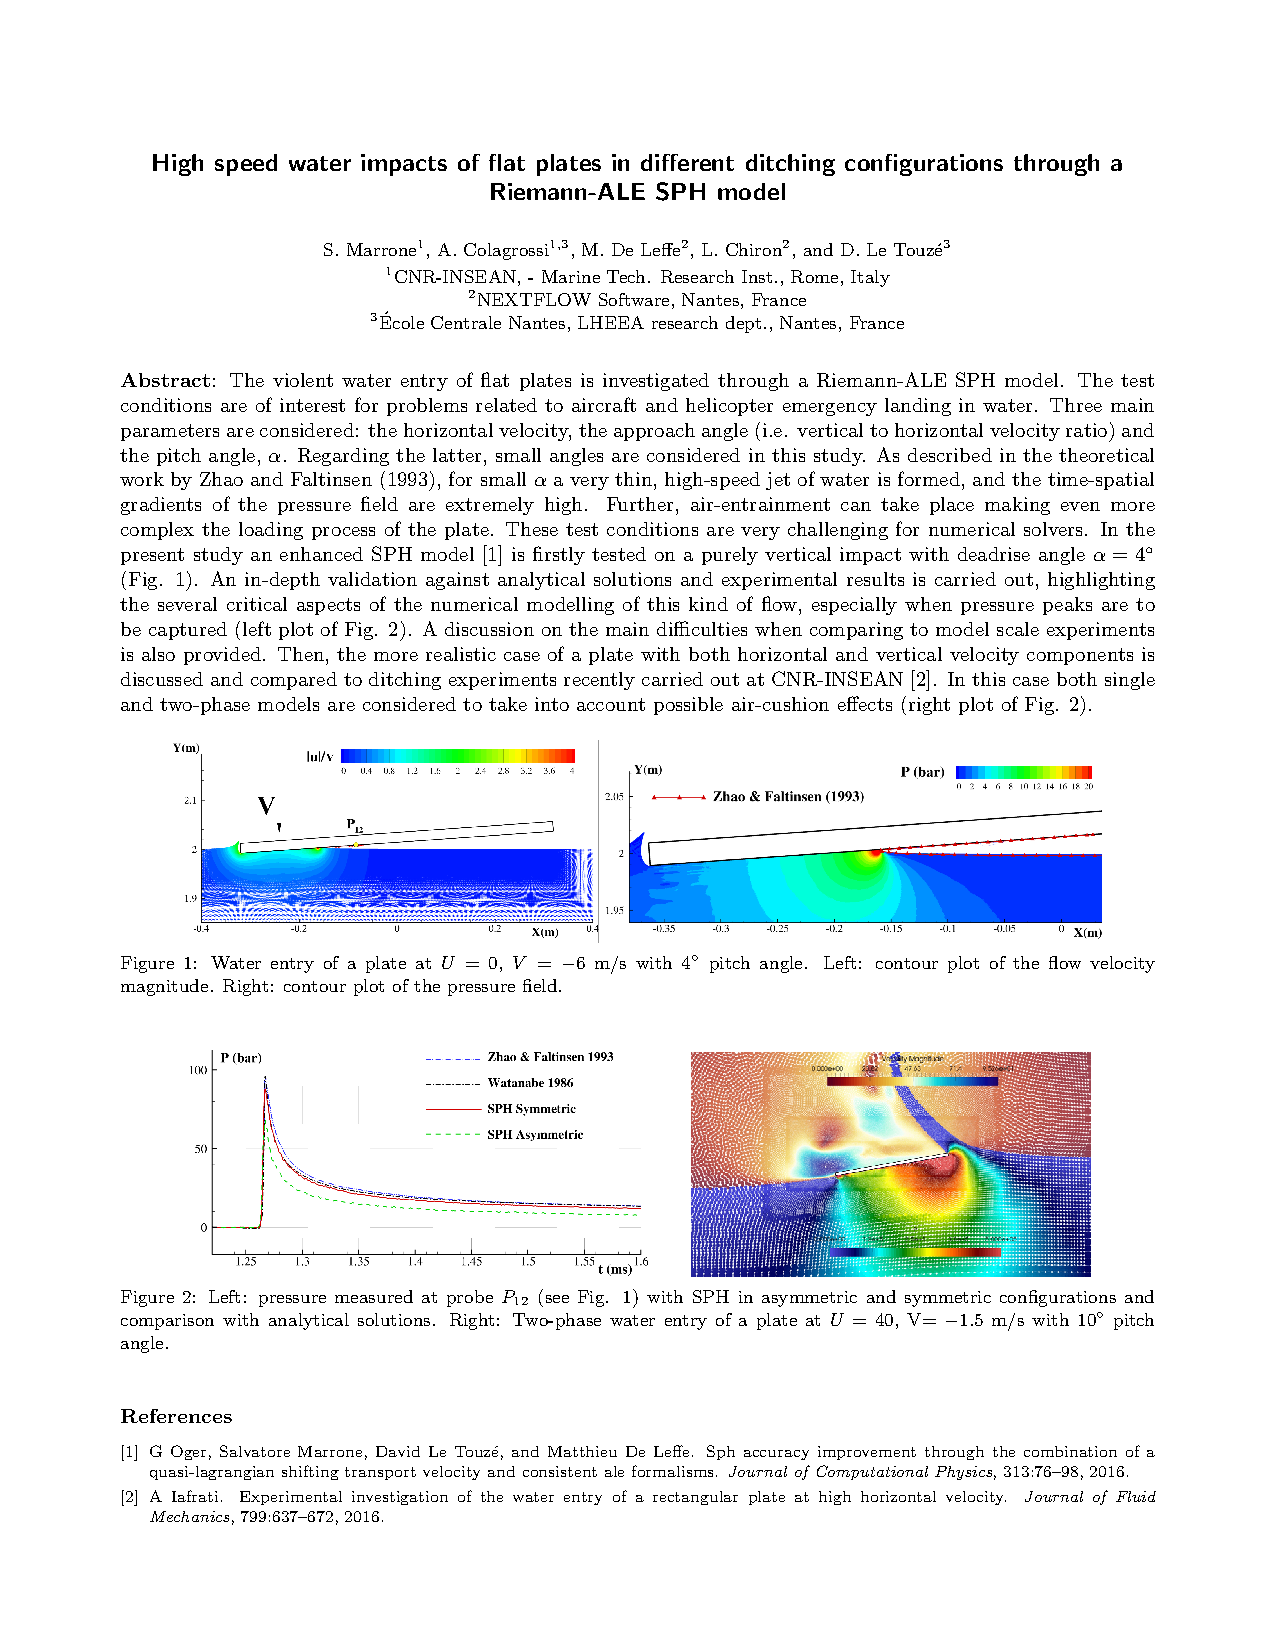
\includepdf[pages=-,pagecommand={\pagestyle{fancy}\label{1.2}},addtotoc={
     1,subsection,1,High speed water impacts of fat plates in different ditching configurations through a Riemann-ALE SPH model,p1}]{abstract/pdfs/1.pdf}
%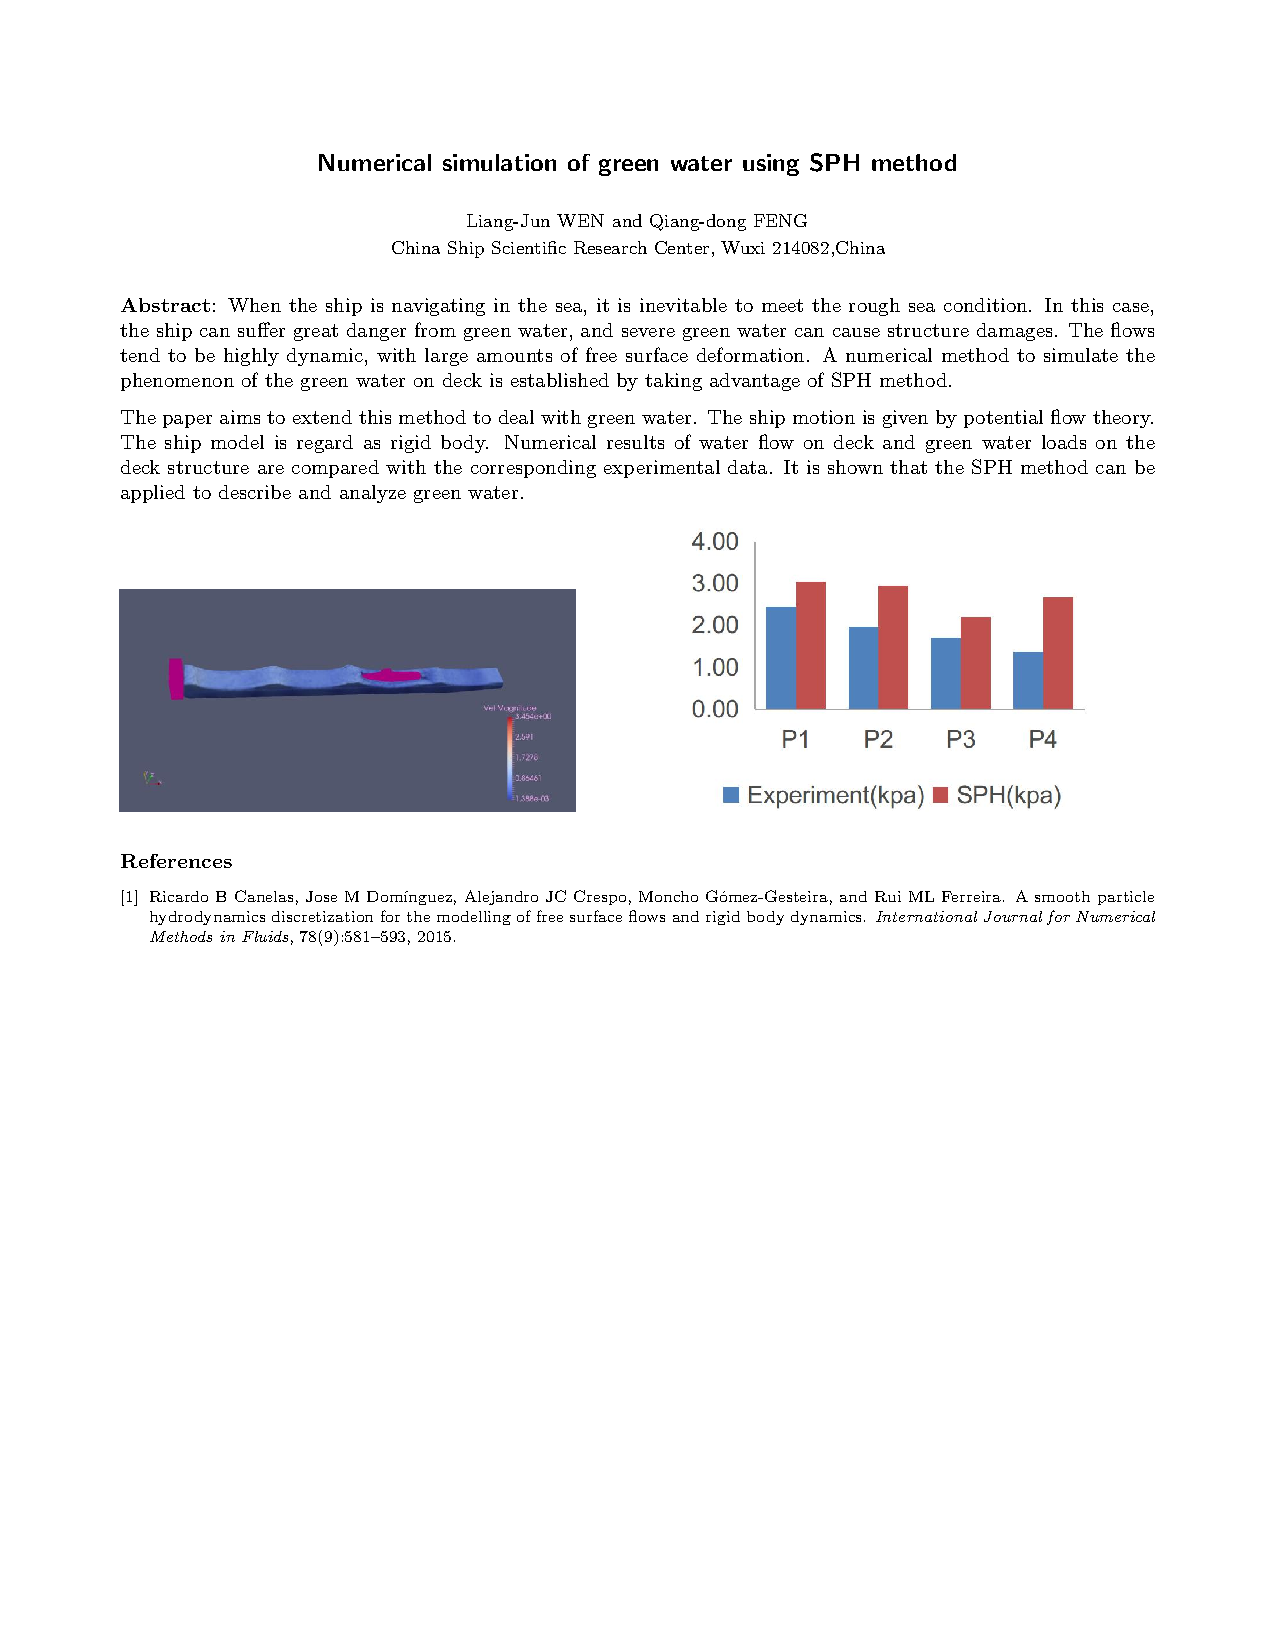
\includepdf[pages=-,pagecommand={\pagestyle{fancy}\label{1.2}},addtotoc={  
%     1,subsection,1,Numerical simulation of green water using SPH method,p1}]{abstract/pdfs/32.pdf}
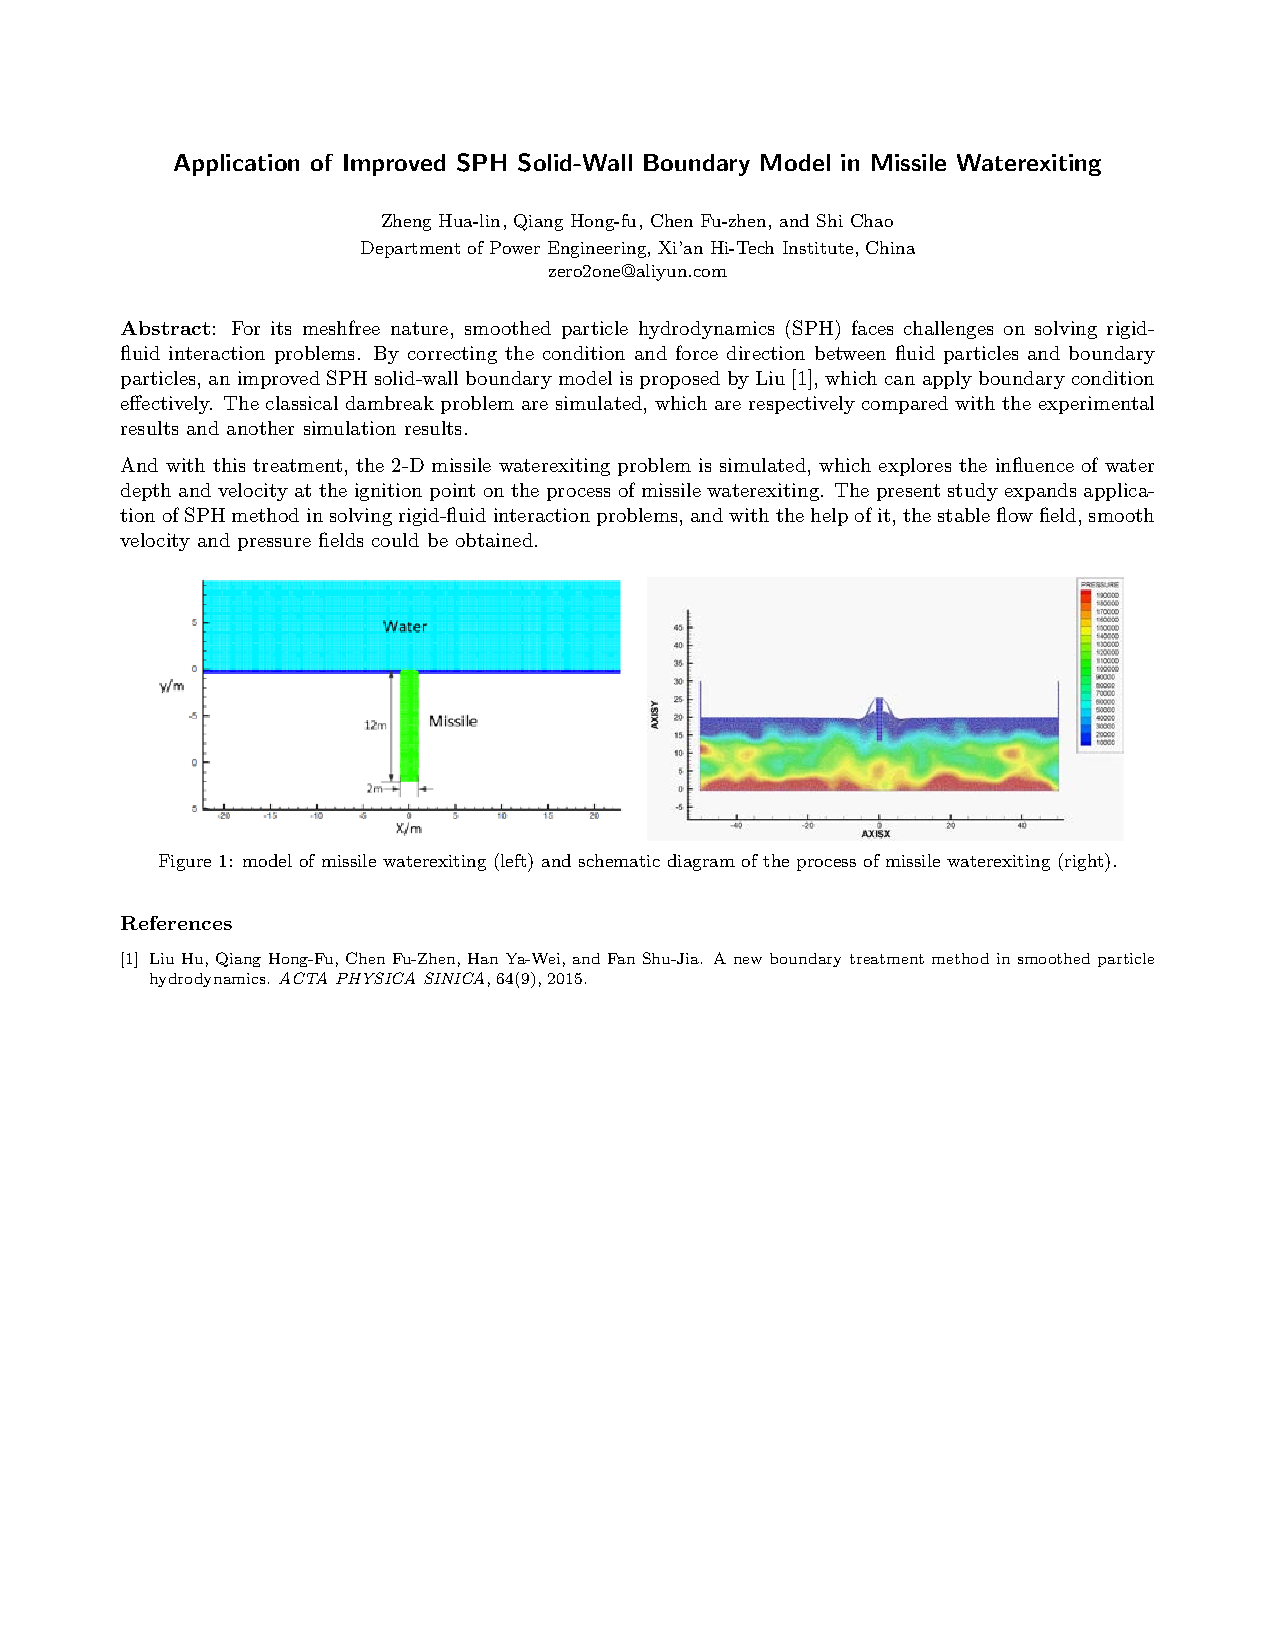
\includepdf[pages=-,pagecommand={\pagestyle{fancy}\label{1.3}},addtotoc={  
     1,subsection,1,Application of improved SPH solid-wall boundary model in missile waterexiting,p1}]{abstract/pdfs/36.pdf}


%\section{Session 2: Multiple Continua and Multi-Phase Flows}
%2.1: 24
%2.2: 31
%2.3: 39
%2.4: 21

\rhead{Session 2}
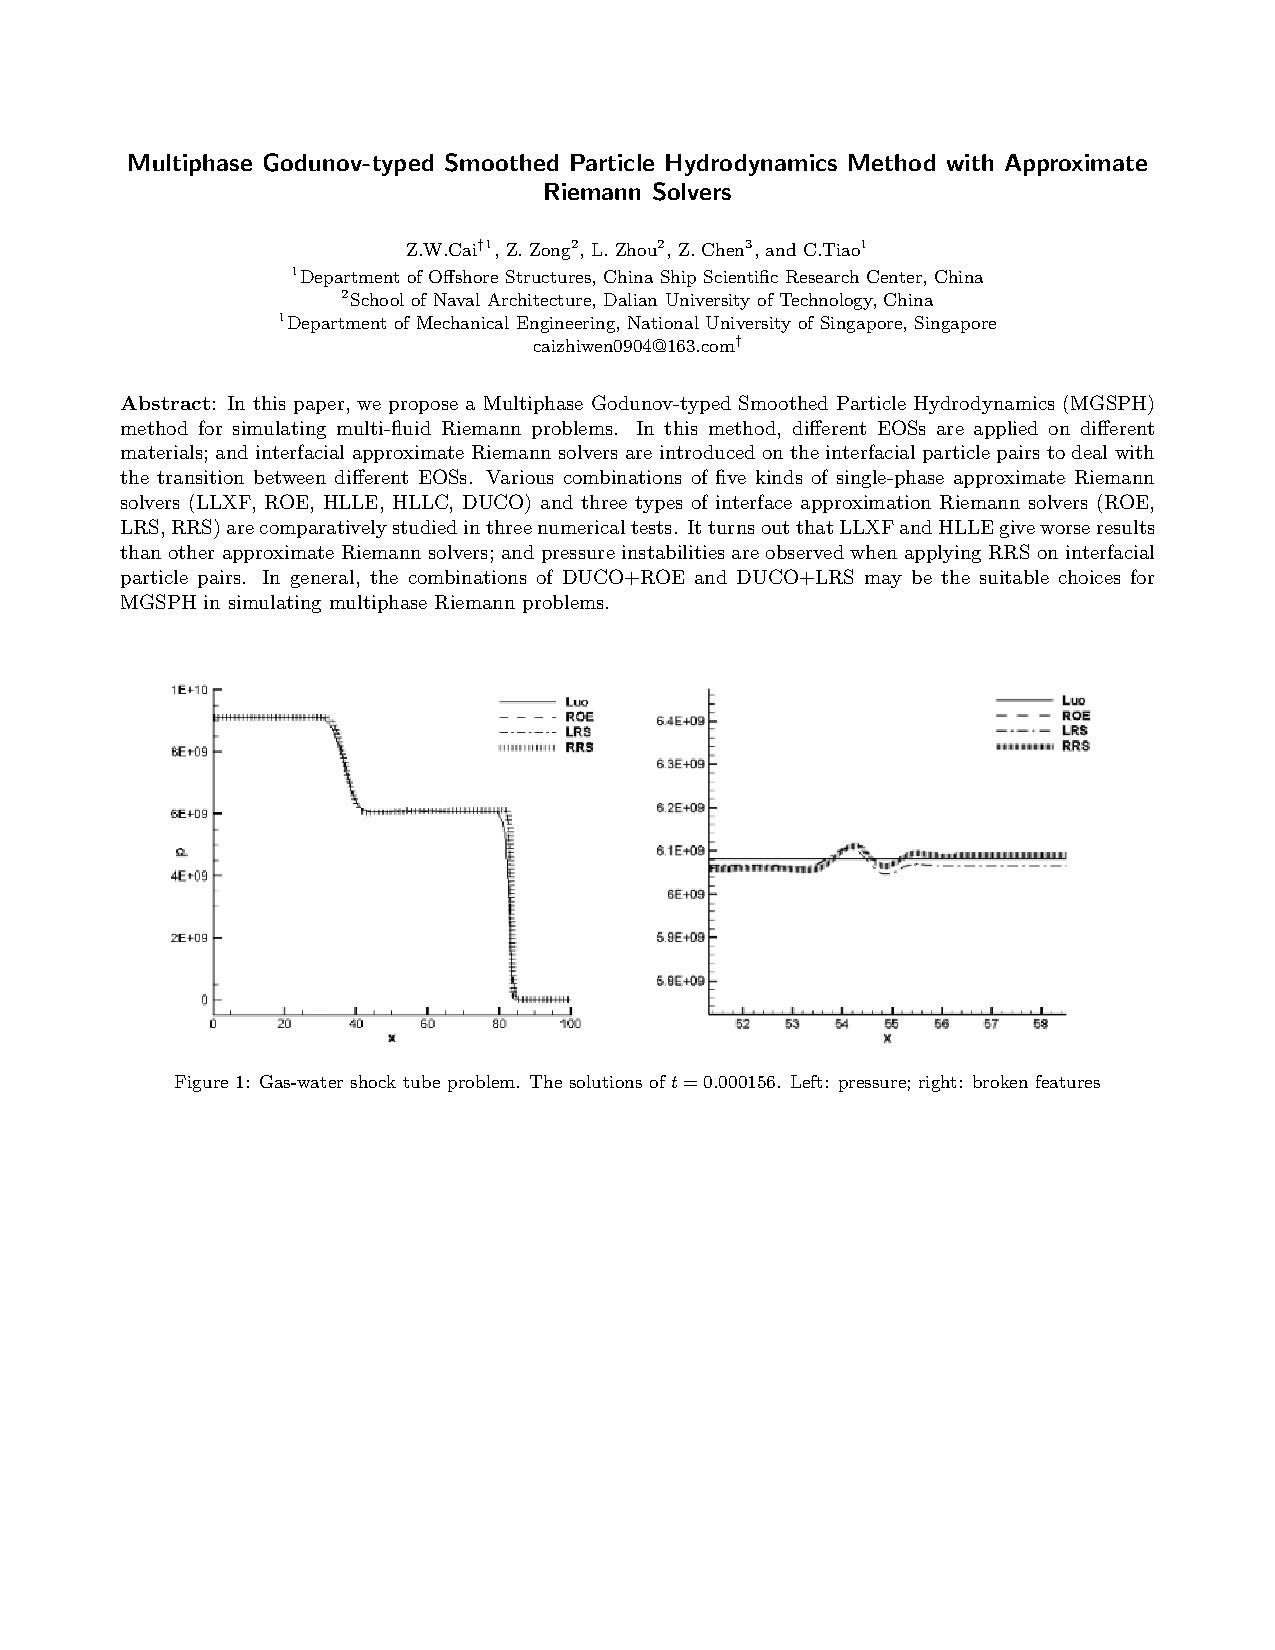
\includepdf[pages=-,pagecommand={\pagestyle{fancy}\label{2.1}},addtotoc={
     1,section,1,{~~~~~~~~Multiple Continua and Multi-Phase Flows},p1,   
     1,subsection,1,Multiphase Godunov-typed smoothed particle hydrodynamics method with approximate Riemann solvers,p1}]{abstract/pdfs/24.pdf}
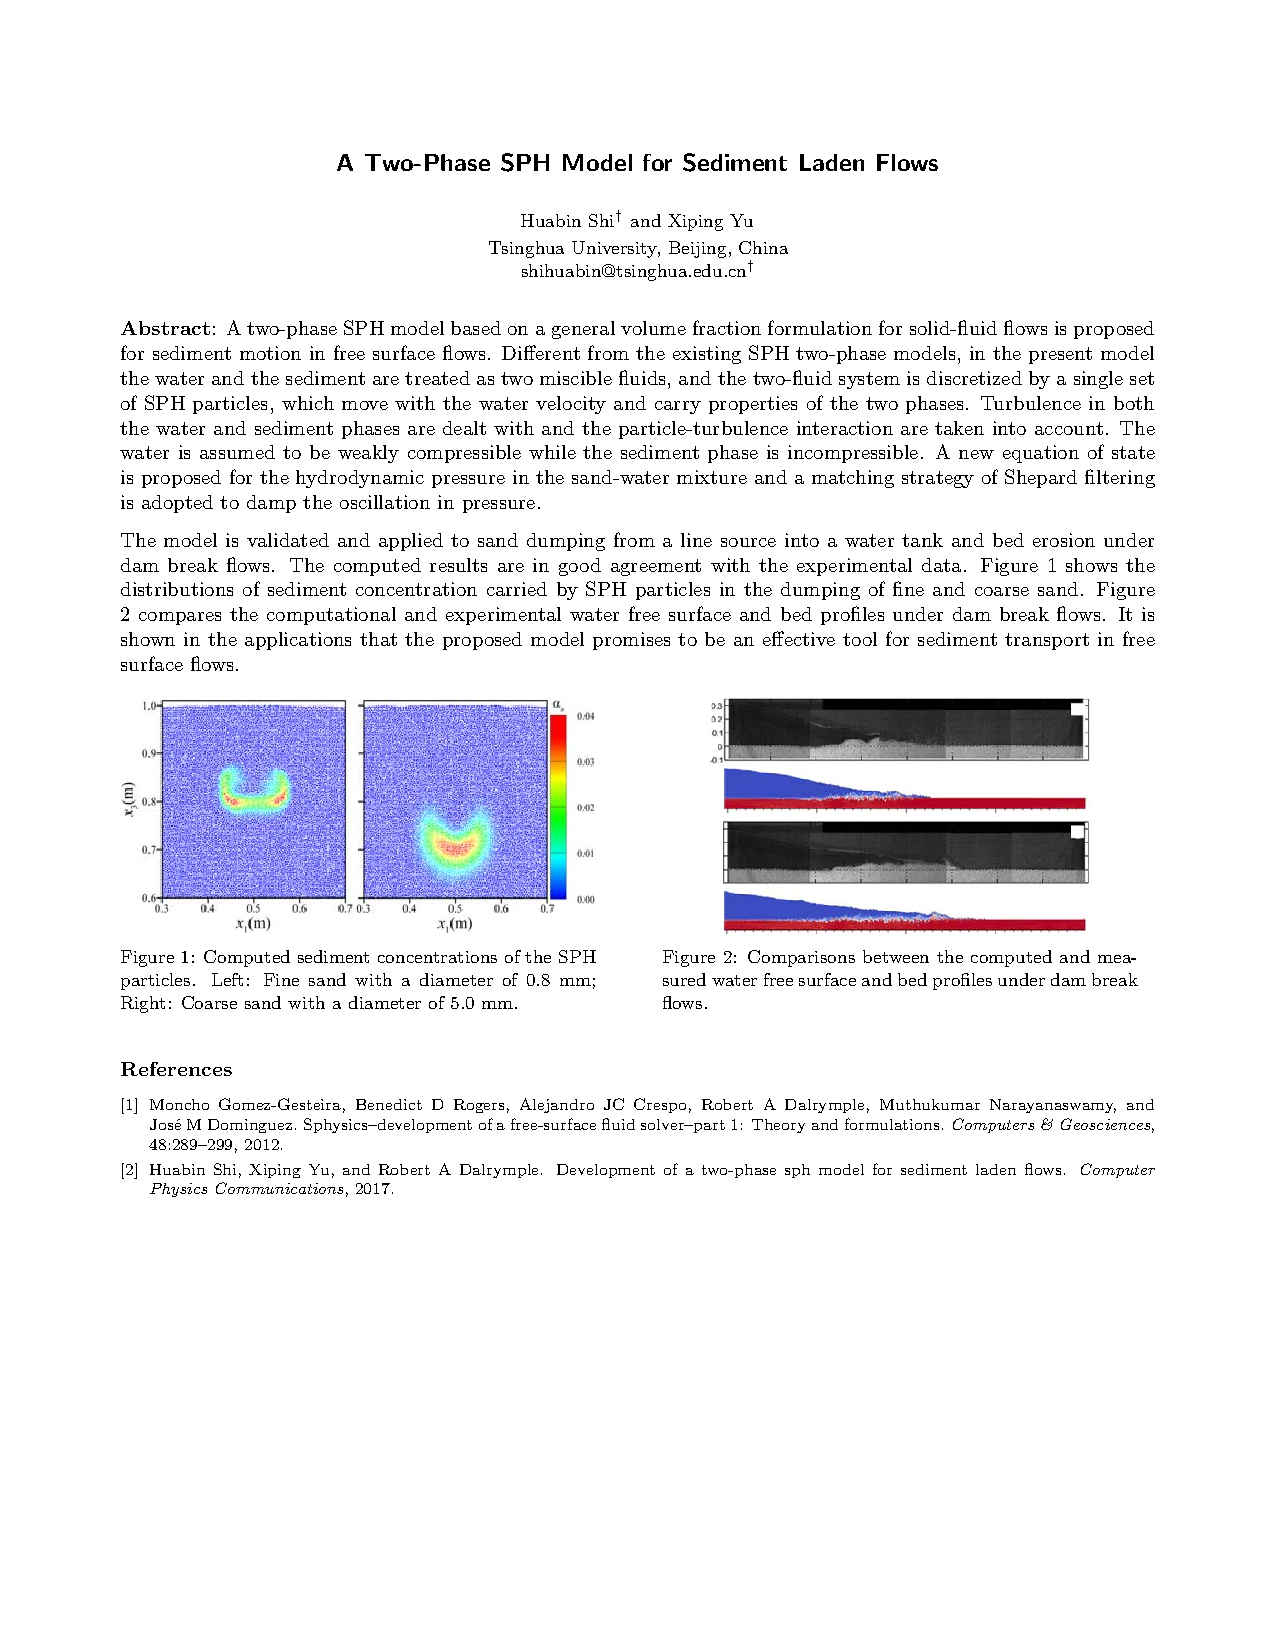
\includepdf[pages=-,pagecommand={\pagestyle{fancy}\label{2.2}},addtotoc={  
     1,subsection,1,A two-phase SPH model for sediment laden flows,p1}]{abstract/pdfs/31.pdf}
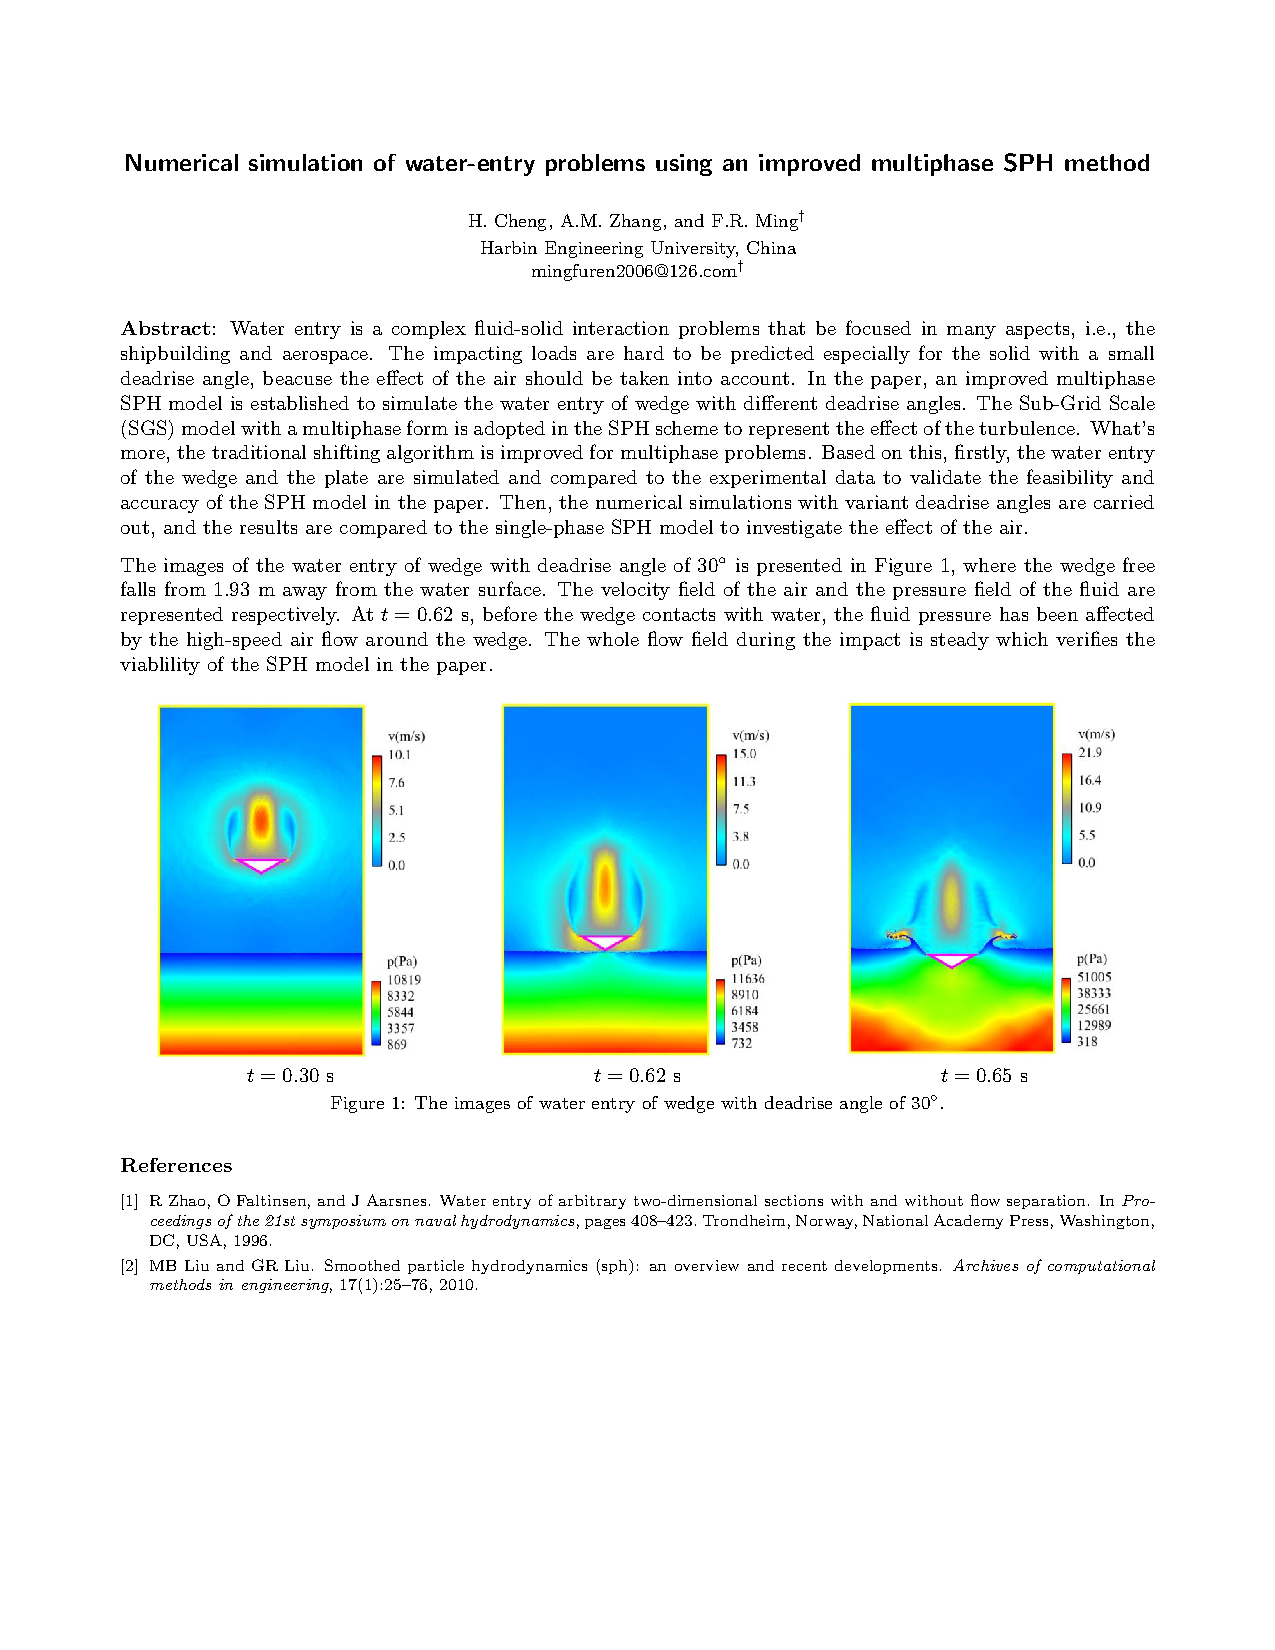
\includepdf[pages=-,pagecommand={\pagestyle{fancy}\label{2.3}},addtotoc={  
     1,subsection,1,Numerical simulation of water-entry problems using an improved multiphase SPH method,p1}]{abstract/pdfs/39.pdf}
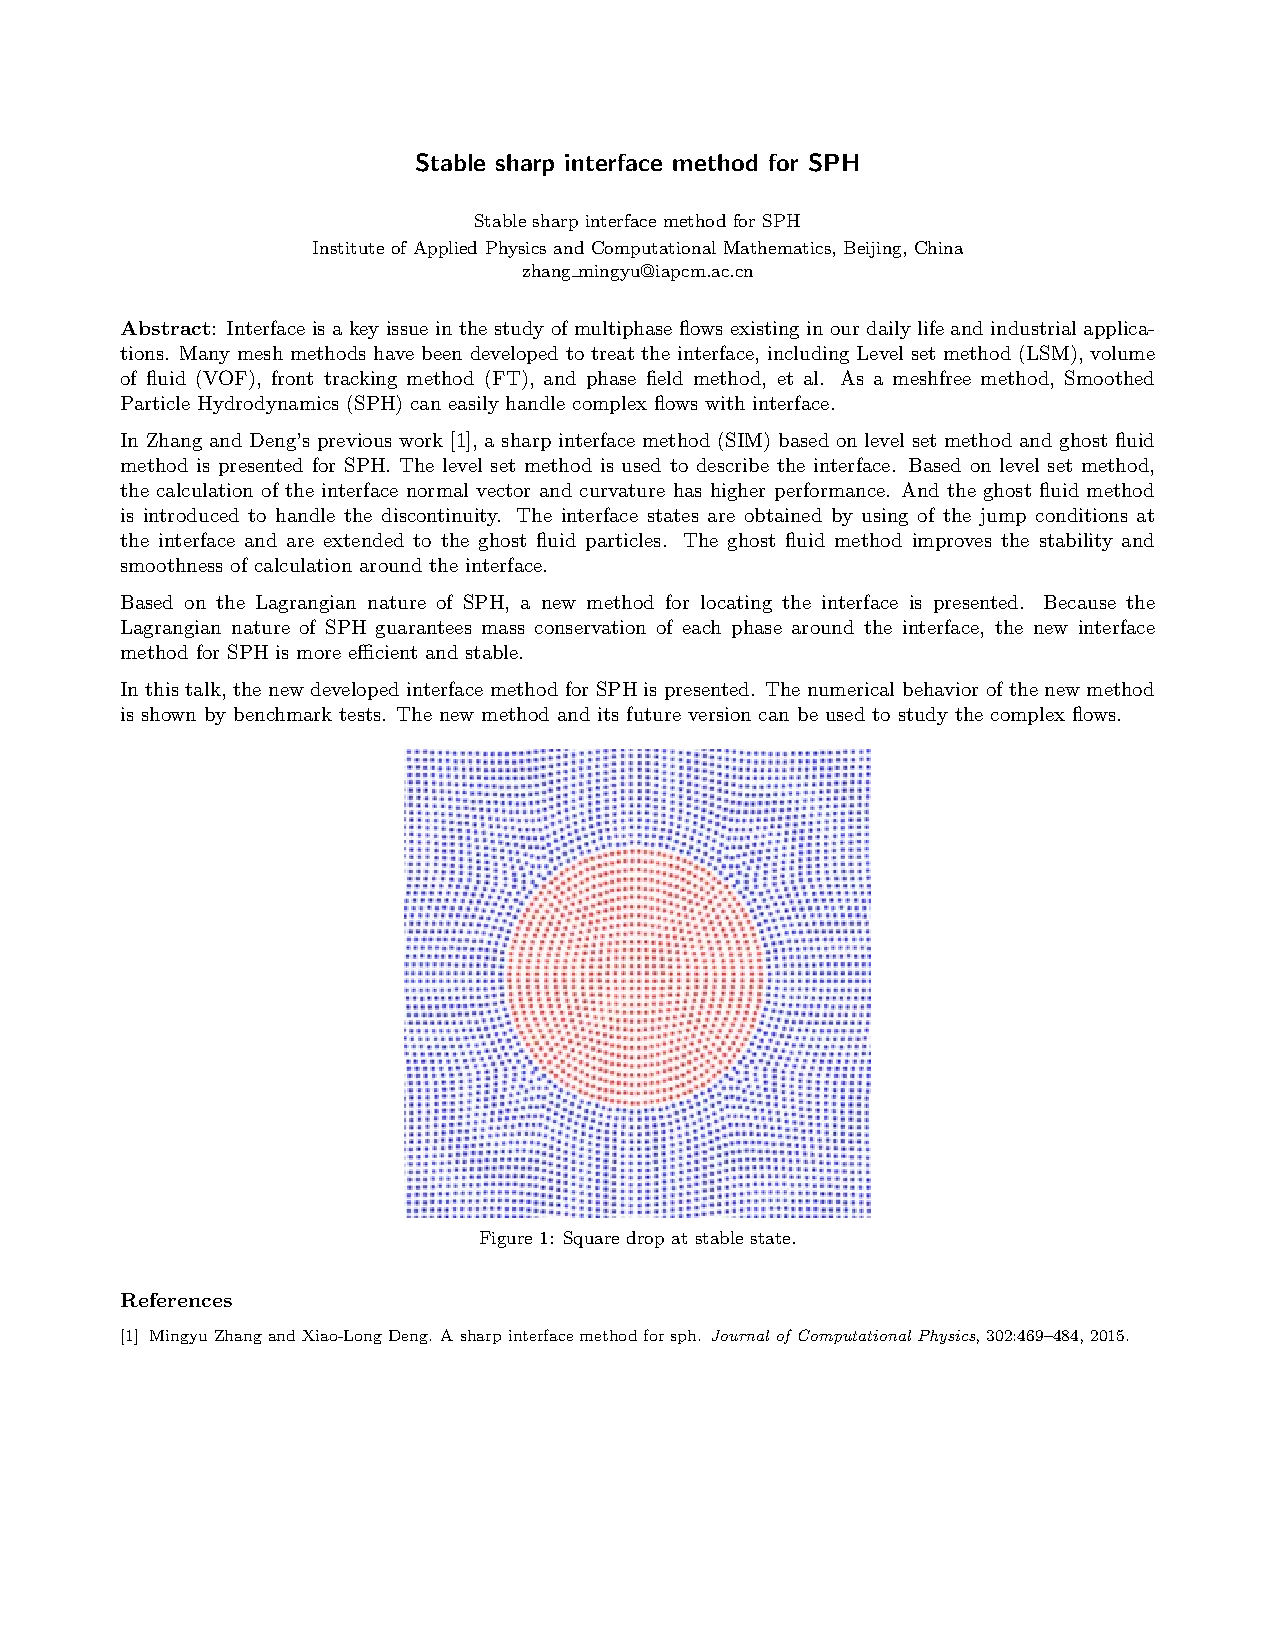
\includepdf[pages=-,pagecommand={\pagestyle{fancy}\label{2.4}},addtotoc={  
     1,subsection,1,Stable sharp interface method for SPH,p1}]{abstract/pdfs/21.pdf}

%\section{Session 3: Impacts with Fluids or Solids}
%3.1: 30
%3.2: 37
%3.3: 41
%3.4: 57

\rhead{Session 3}
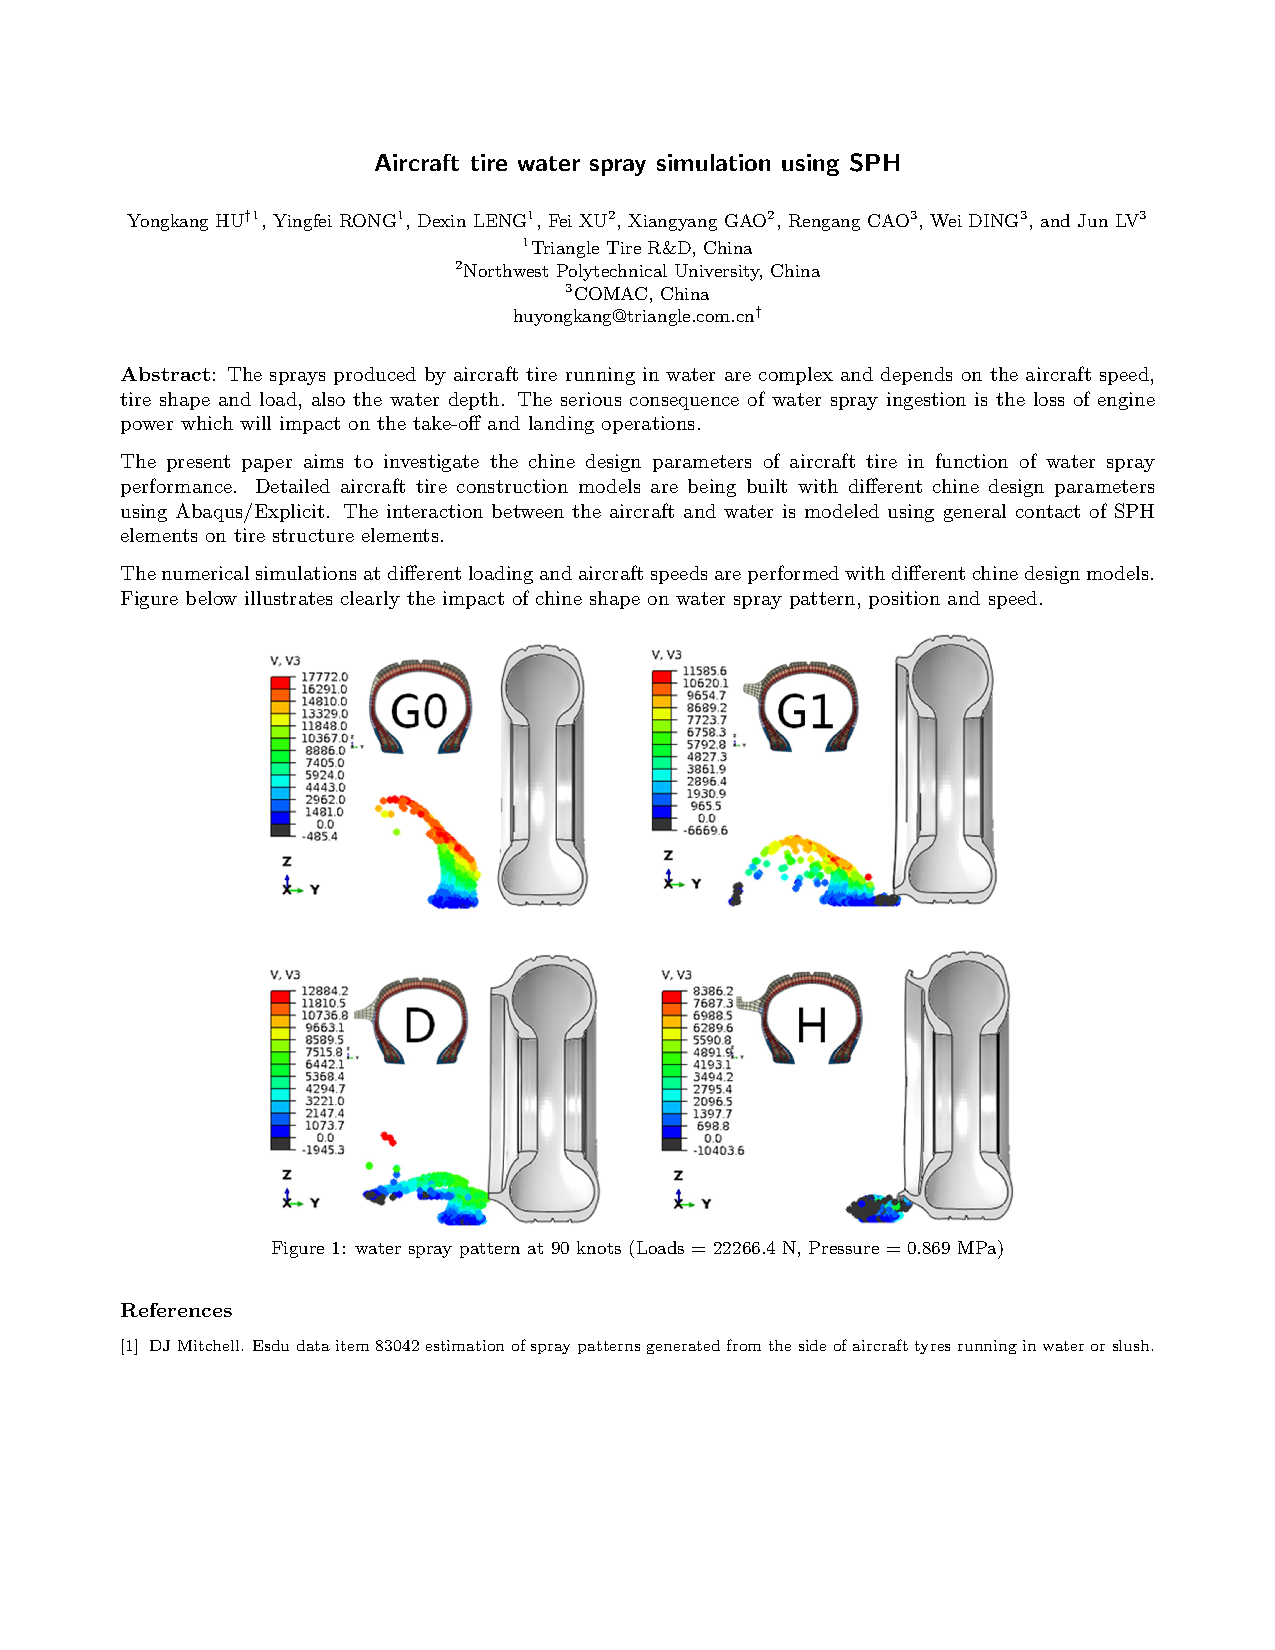
\includepdf[pages=-,pagecommand={\pagestyle{fancy}\label{3.1}},addtotoc={
     1,section,1,{~~~~~~~~Impacts with Fluids or Solids},p1,   
     1,subsection,1,Aircraft tire water spray simulation using SPH,p1}]{abstract/pdfs/30.pdf}
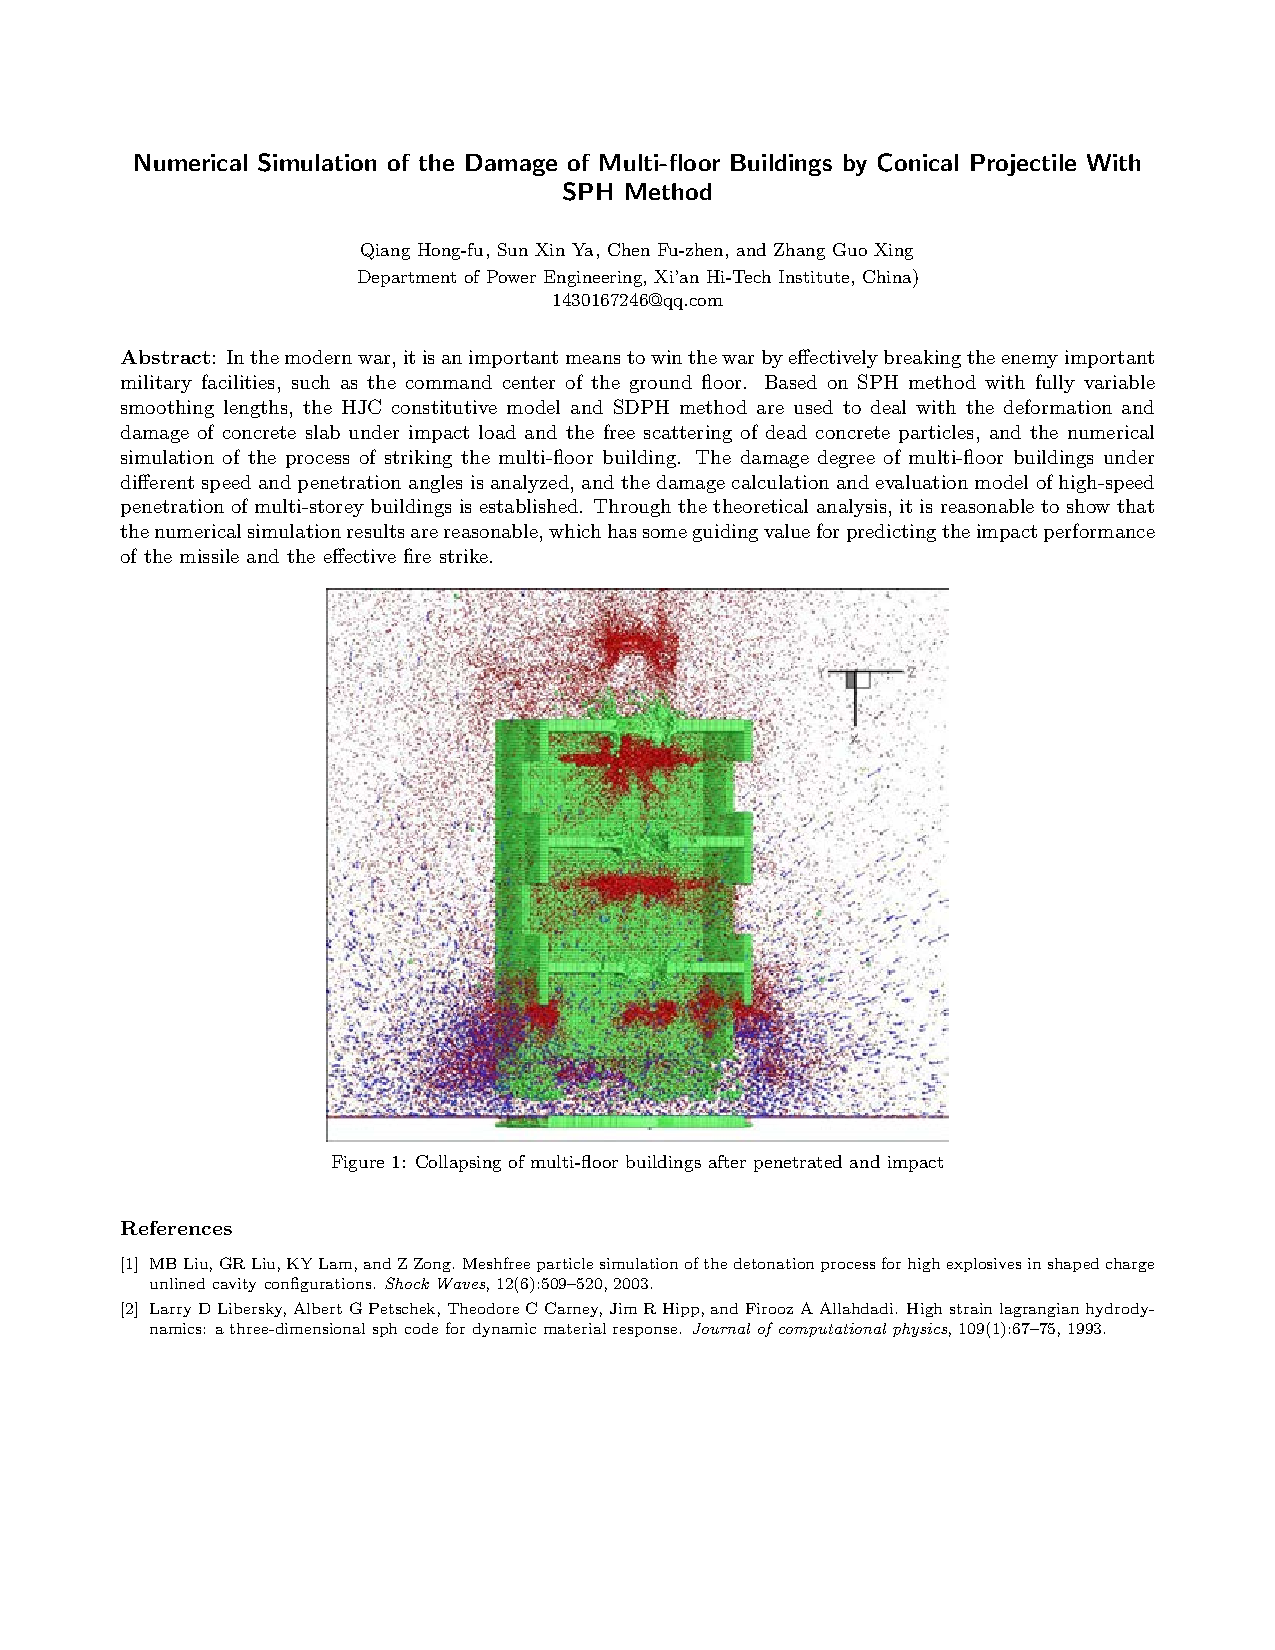
\includepdf[pages=-,pagecommand={\pagestyle{fancy}\label{3.2}},addtotoc={  
     1,subsection,1,Numerical simulation of the damage of multi-floor buildings by conical projectile with SPH method,p1}]{abstract/pdfs/37.pdf}
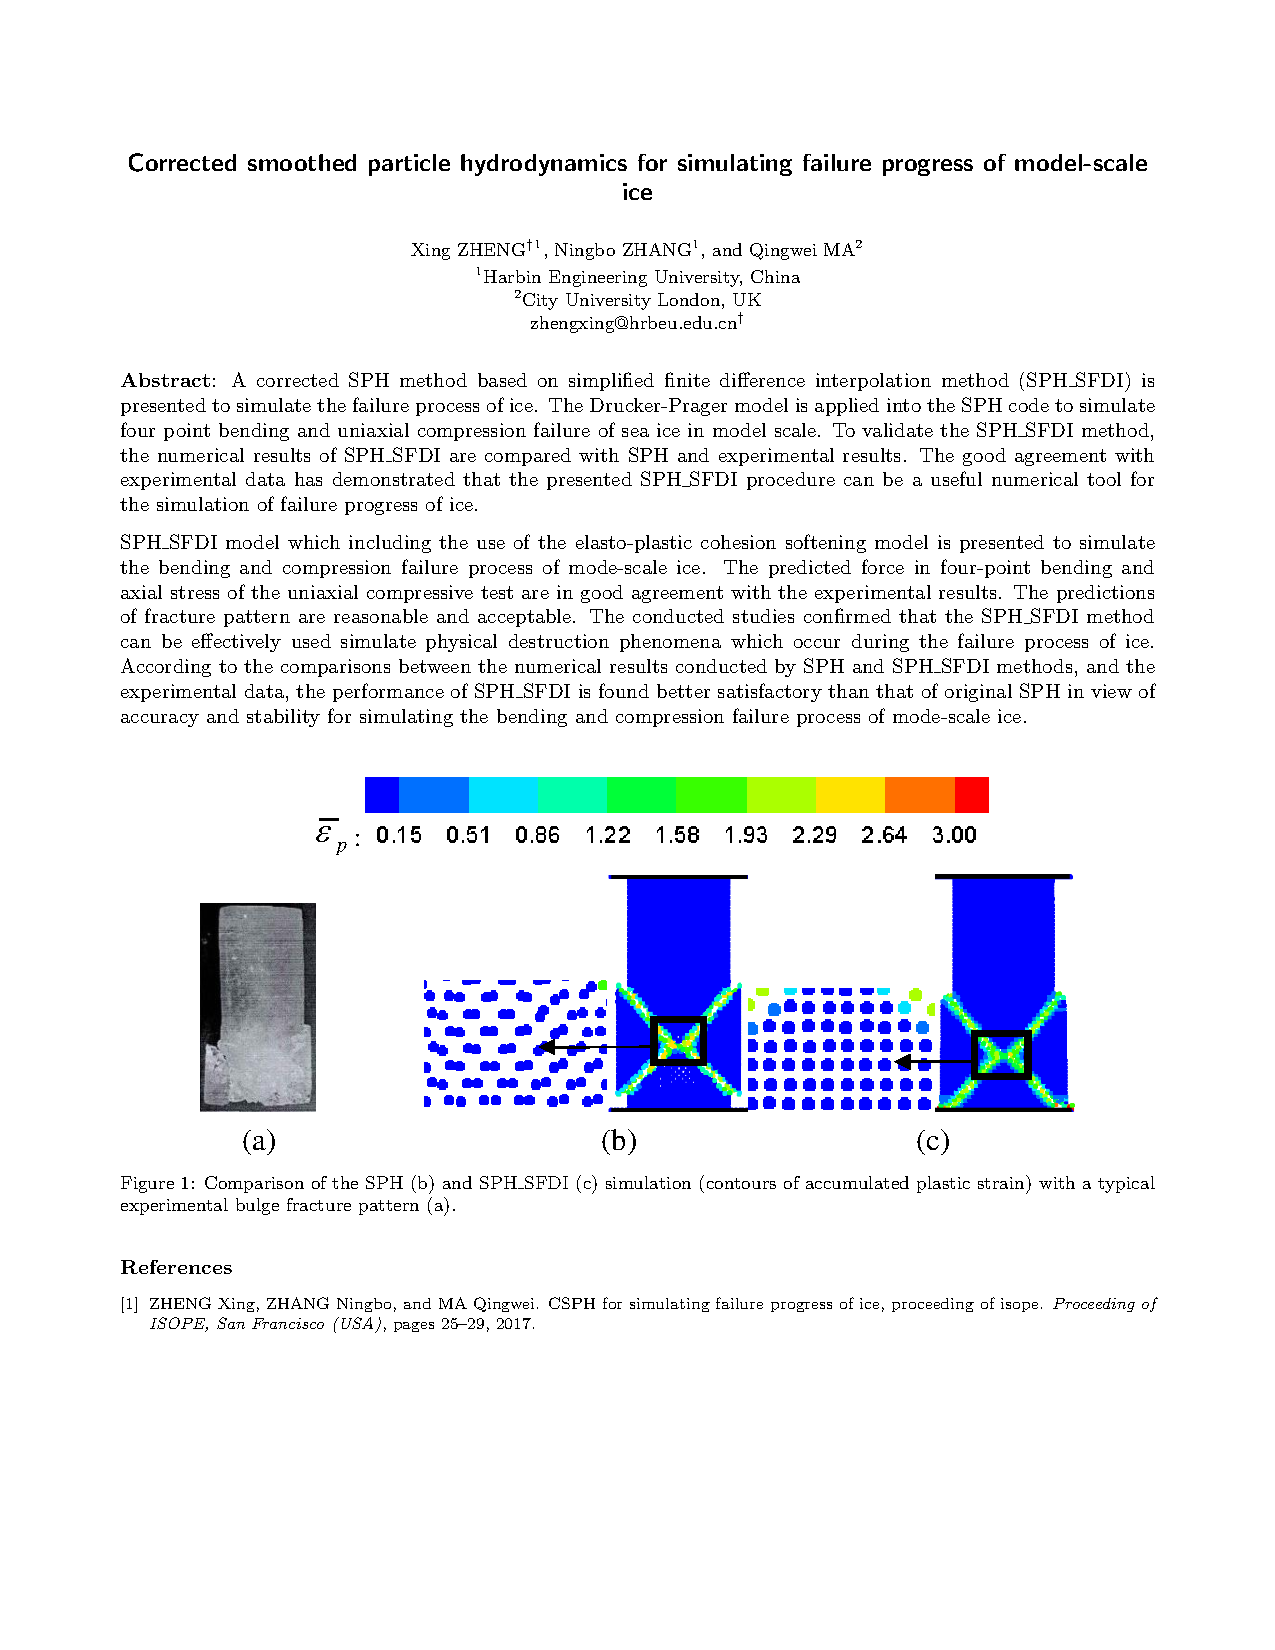
\includepdf[pages=-,pagecommand={\pagestyle{fancy}\label{3.3}},addtotoc={  
     1,subsection,1,Corrected smoothed particle hydrodynamics for simulating failure progress of model-scale ice,p1}]{abstract/pdfs/41.pdf}
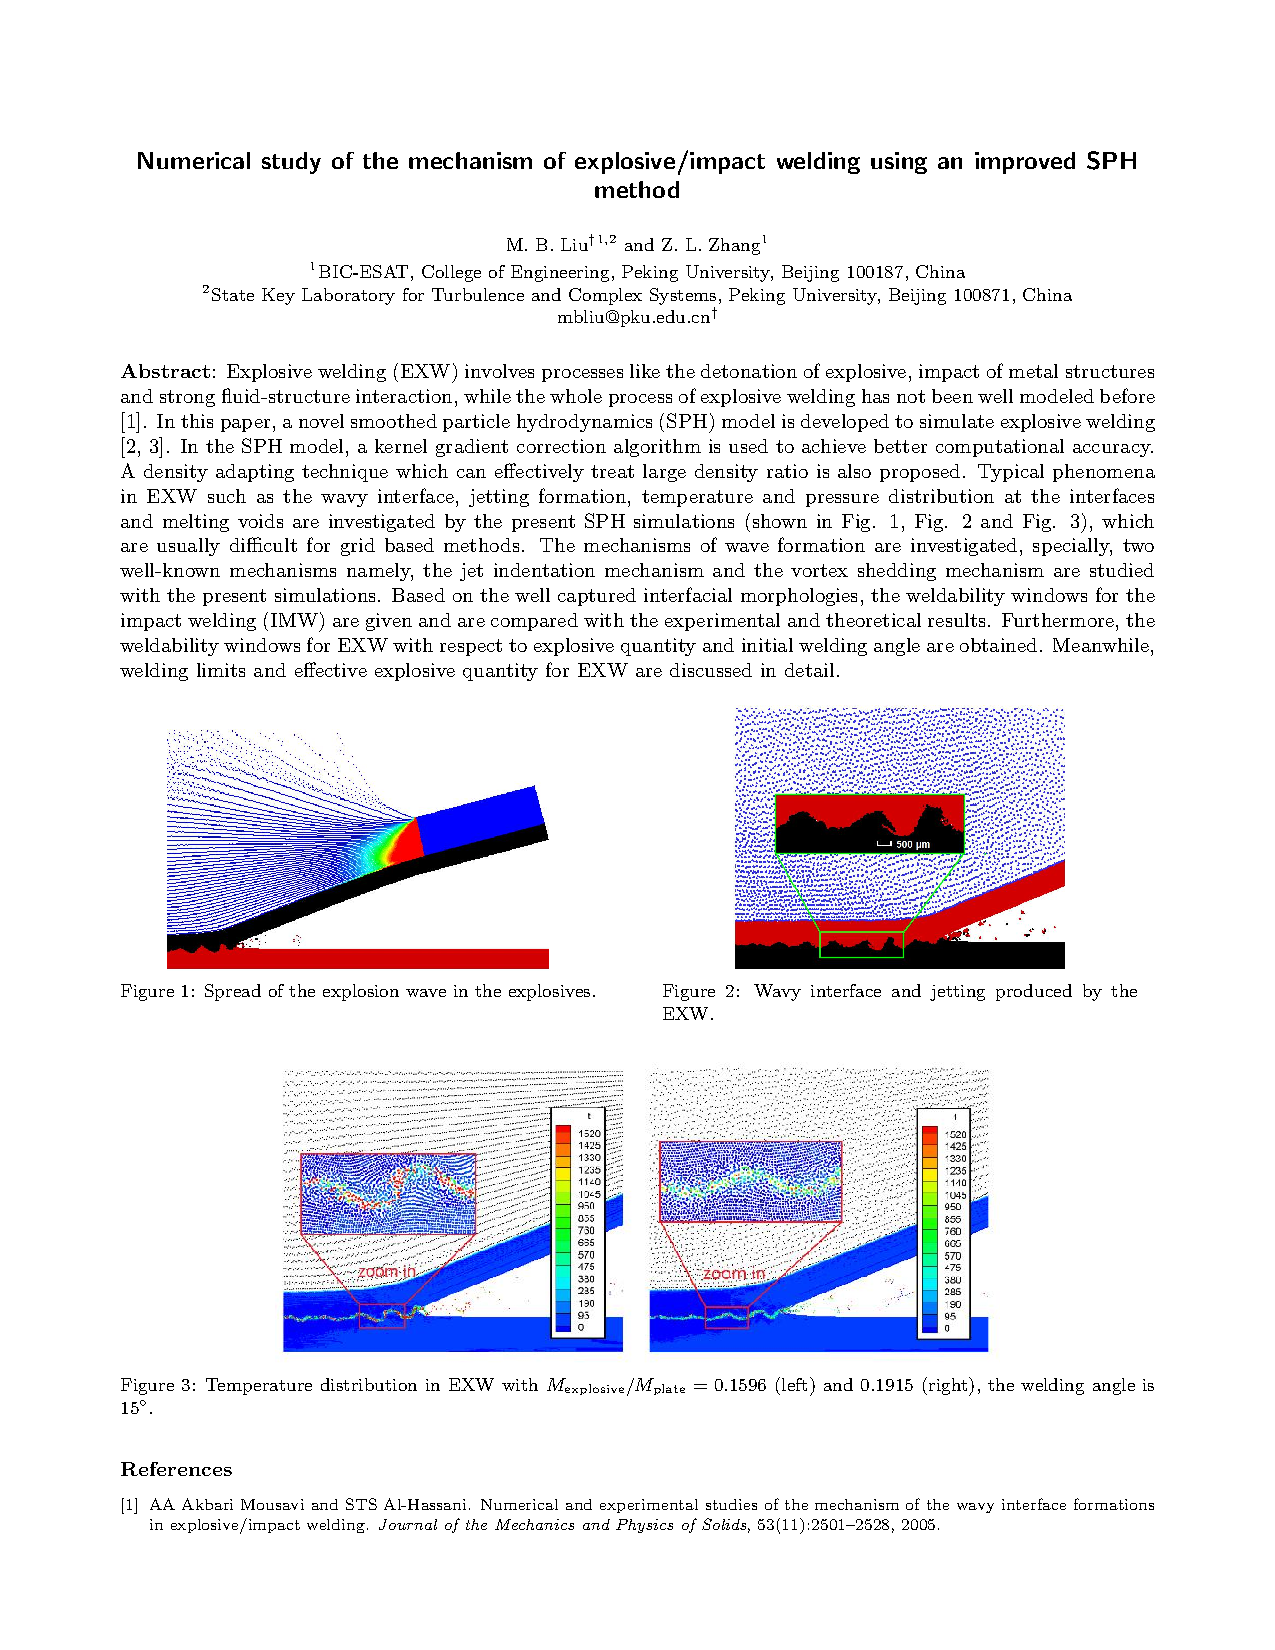
\includepdf[pages=-,pagecommand={\pagestyle{fancy}\label{3.4}},addtotoc={  
     1,subsection,1,Numerical study of the mechanism of explosive/impact welding using an improved SPH method,p1}]{abstract/pdfs/57.pdf}

%\section{Session 4: Free Surface and Moving Boundaries Applications}
%4.1: 1
%4.2: 14
%4.3: 40
%4.4: 44

\rhead{Session 4}
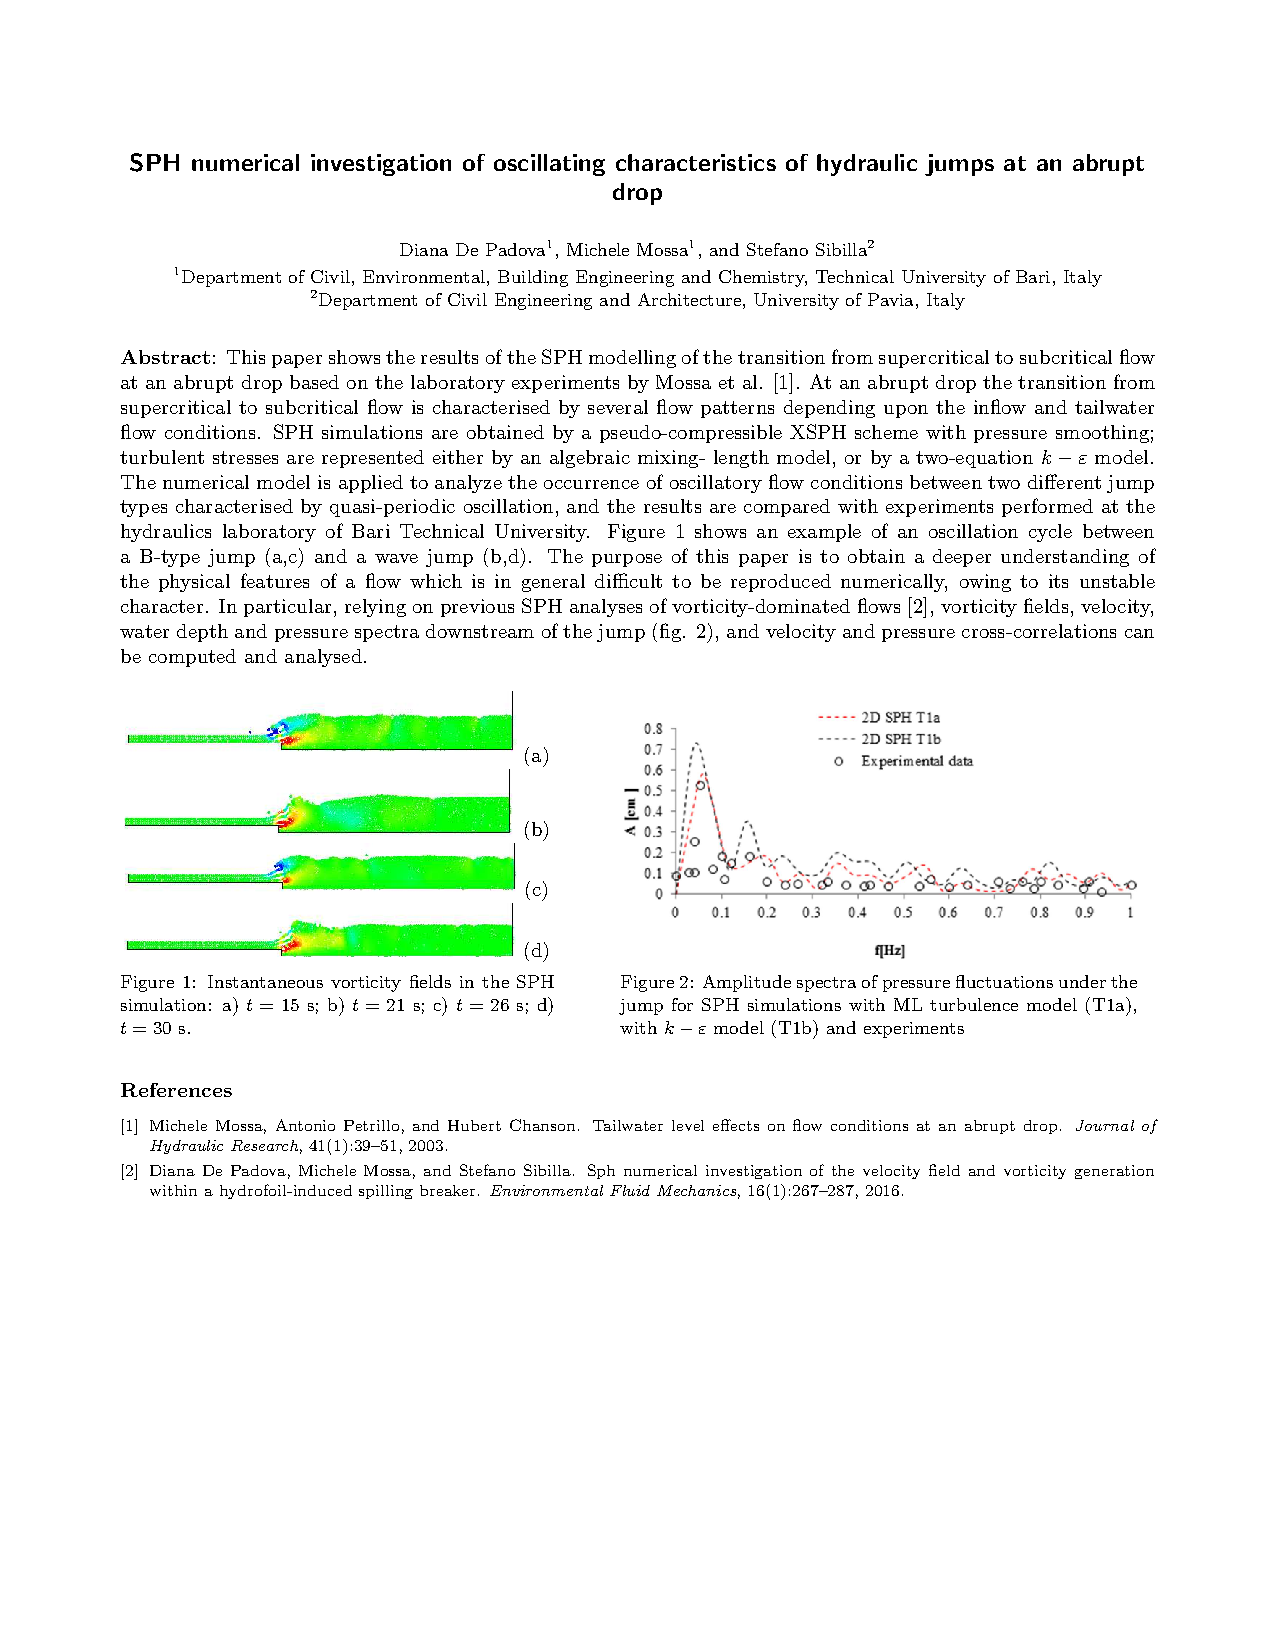
\includepdf[pages=-,pagecommand={\pagestyle{fancy}\label{4.1}},addtotoc={  
     1,section,1,{~~~~~~~~Free Surface and Moving Boundaries Applications},p1,   
     1,subsection,1,SPH numerical investigation of oscillating characteristics of hydraulic jumps at an abrupt drop,p1}]{abstract/pdfs/14.pdf}

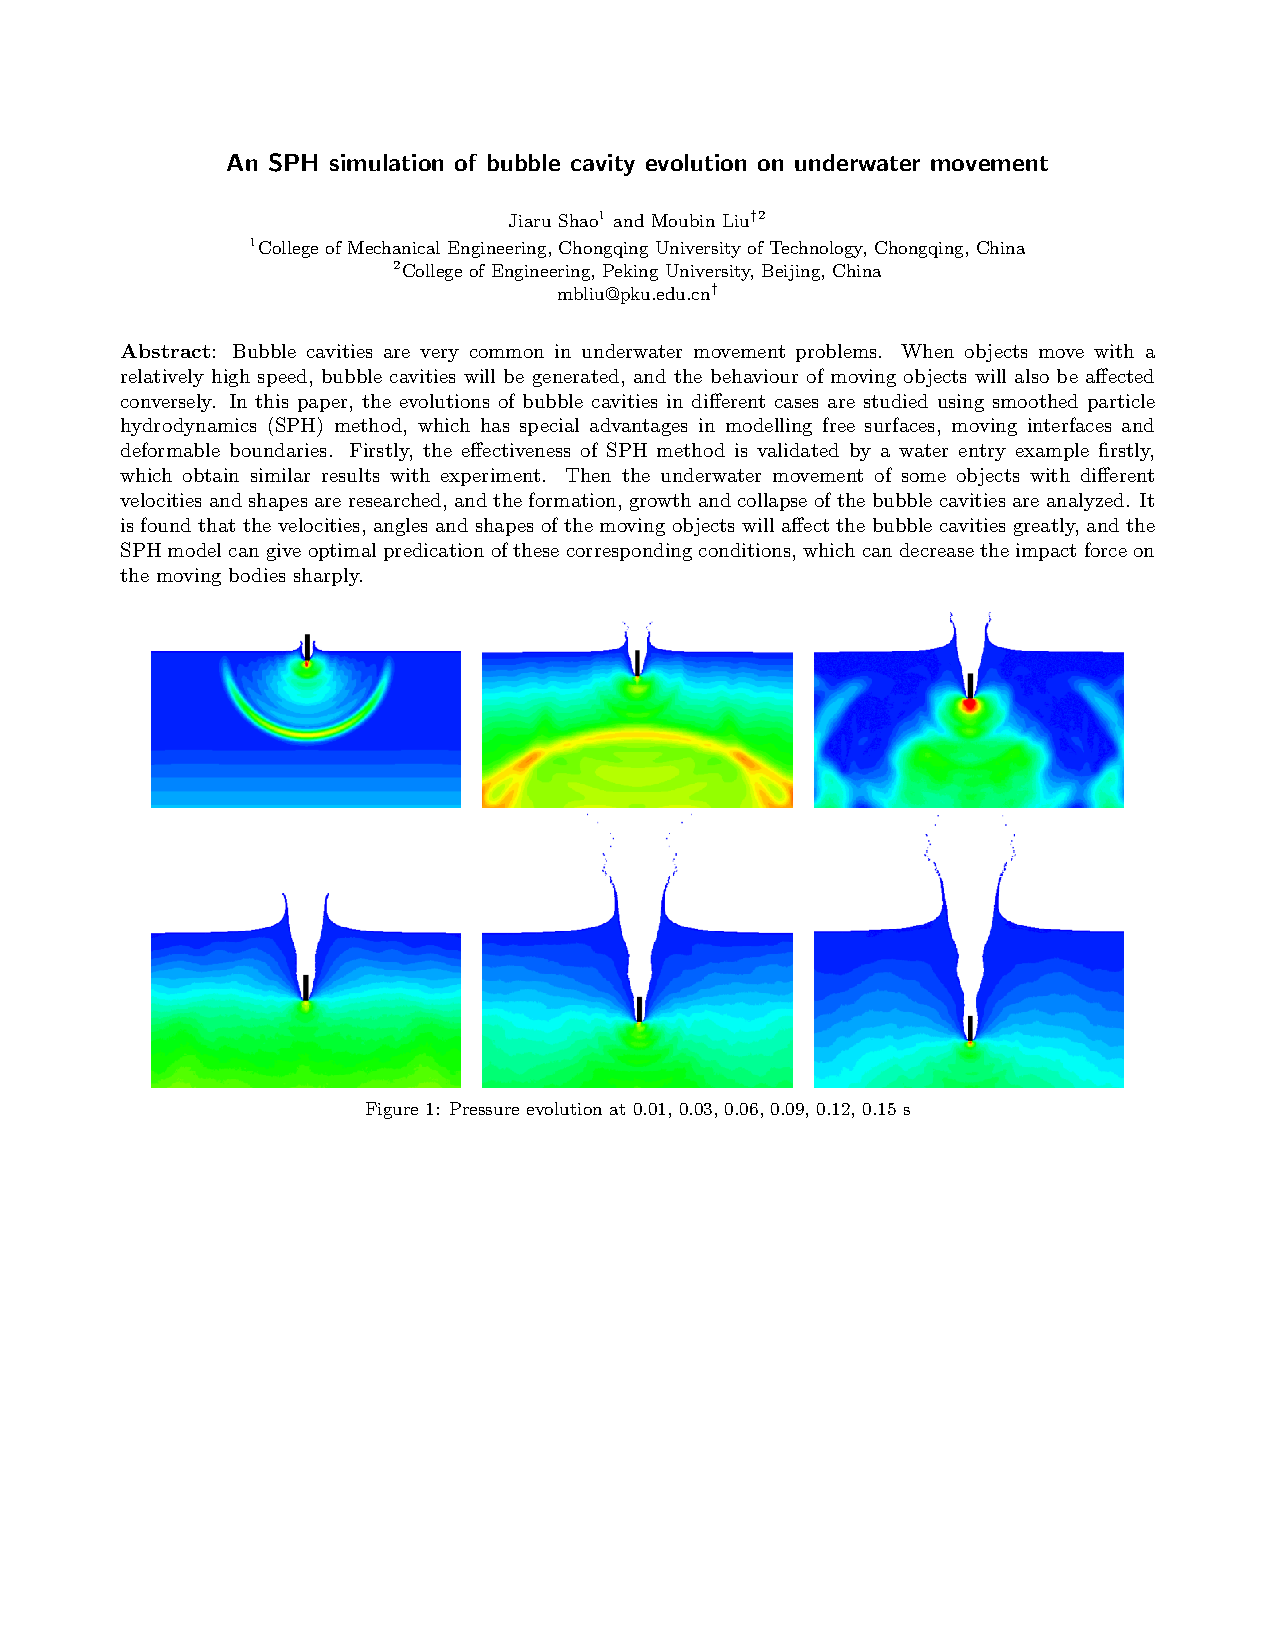
\includepdf[pages=-,pagecommand={\pagestyle{fancy}\label{4.2}},addtotoc={  
     1,subsection,1,An SPH simulation of bubble cavity evolution on underwater movement,p1}]{abstract/pdfs/20.pdf}
     
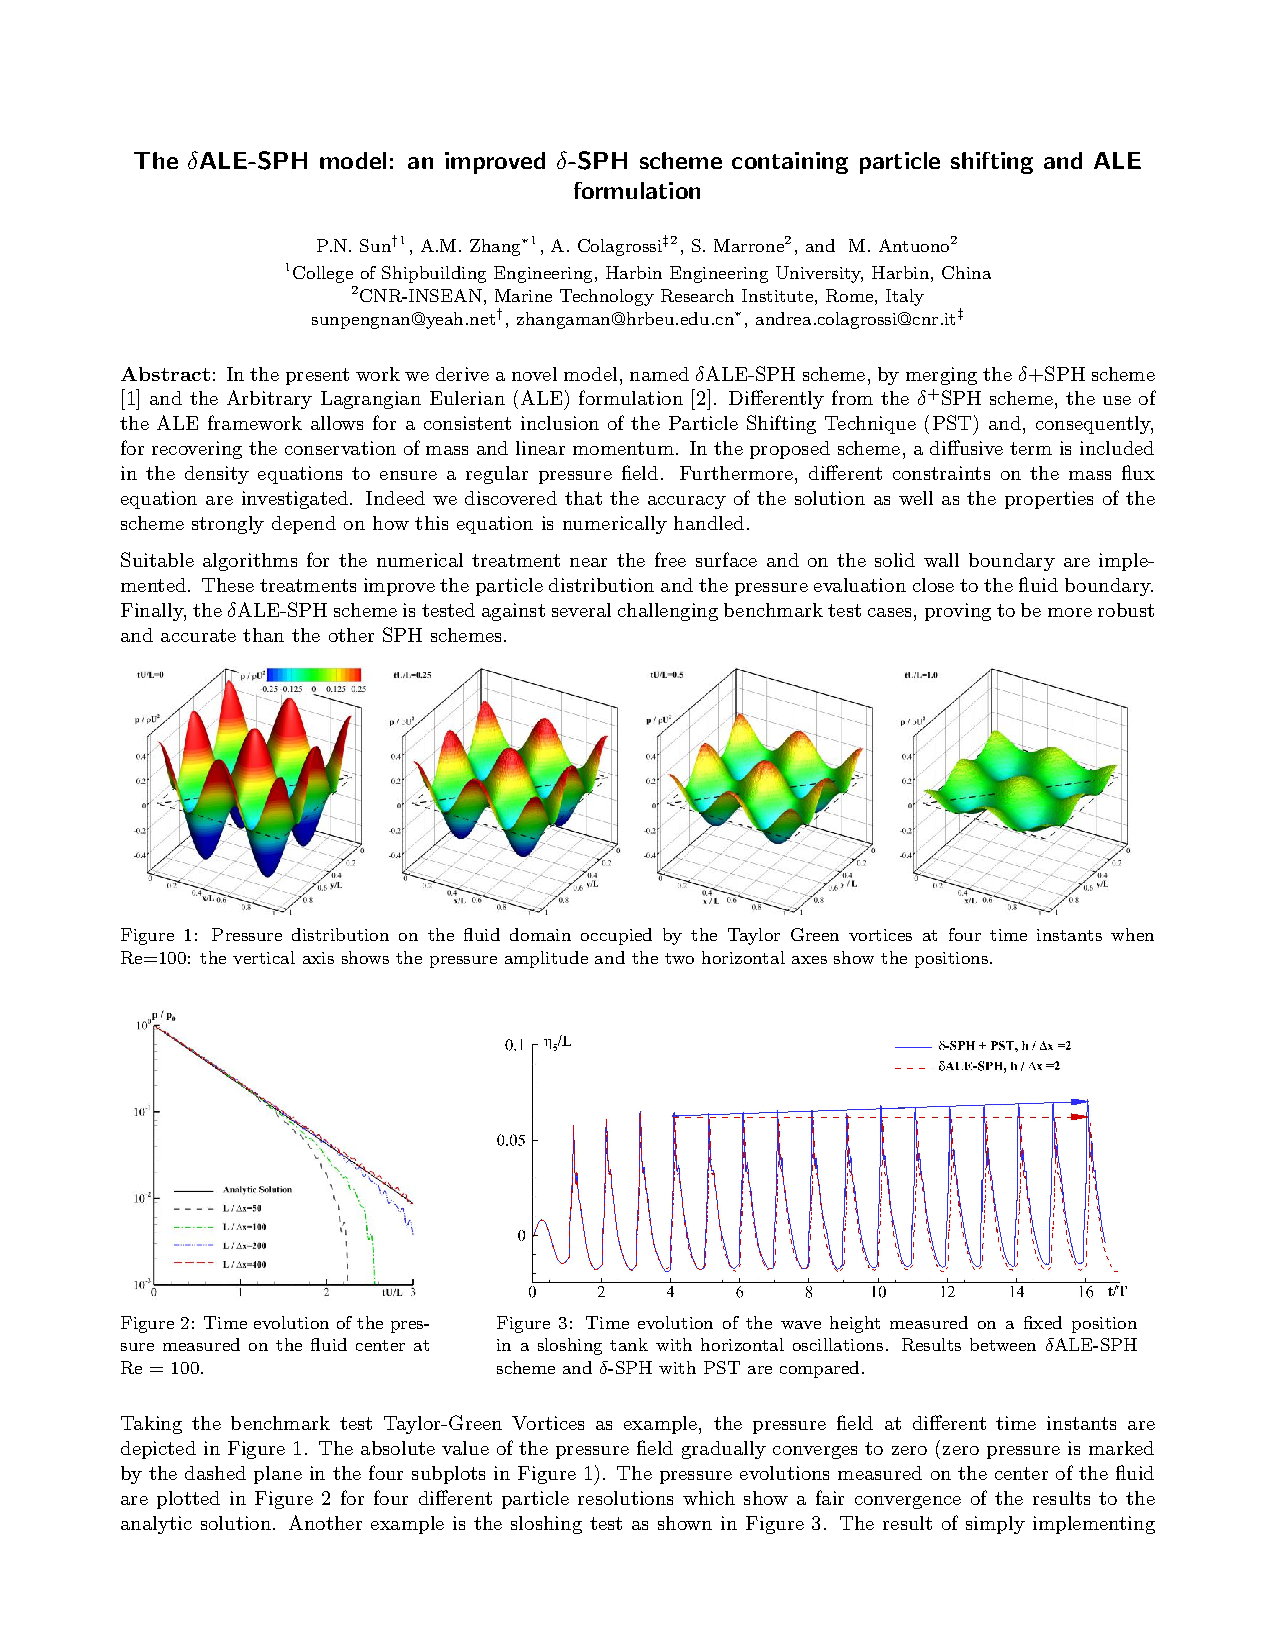
\includepdf[pages=-,pagecommand={\pagestyle{fancy}\label{4.3}},addtotoc={  
     1,subsection,1,The $\delta$ALE-SPH model: an improved $\delta$-SPH scheme containing particle shifting and ALE formulation,p1}]{abstract/pdfs/40.pdf}
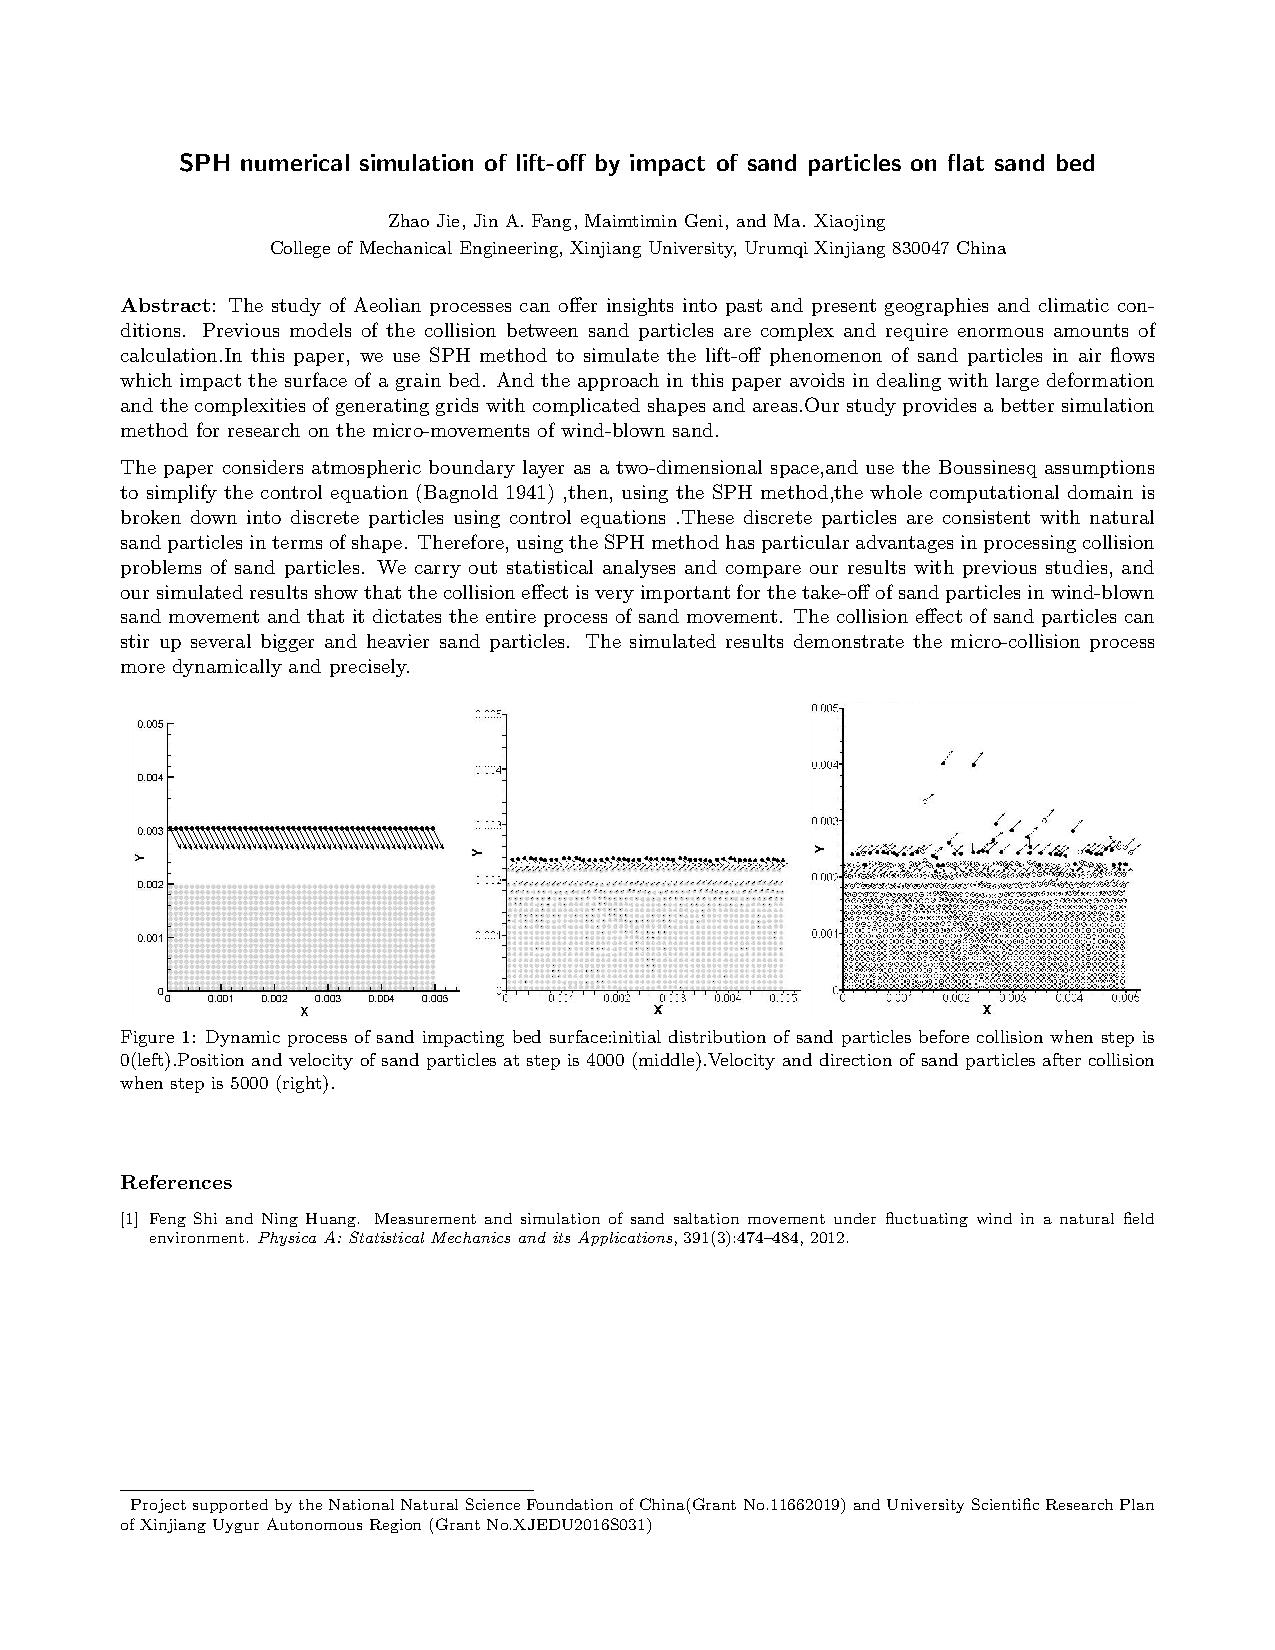
\includepdf[pages=-,pagecommand={\pagestyle{fancy}\label{4.4}},addtotoc={  
     1,subsection,1,SPH numerical simulation of lift-off by impact of sand particles on flat sand bed,p1}]{abstract/pdfs/44.pdf}

%\section{Session 5: Geotechnical  Applications}
%5.1: 4
%5.2: 5
%5.3: 6
%5.4: 33

\rhead{Session 5}
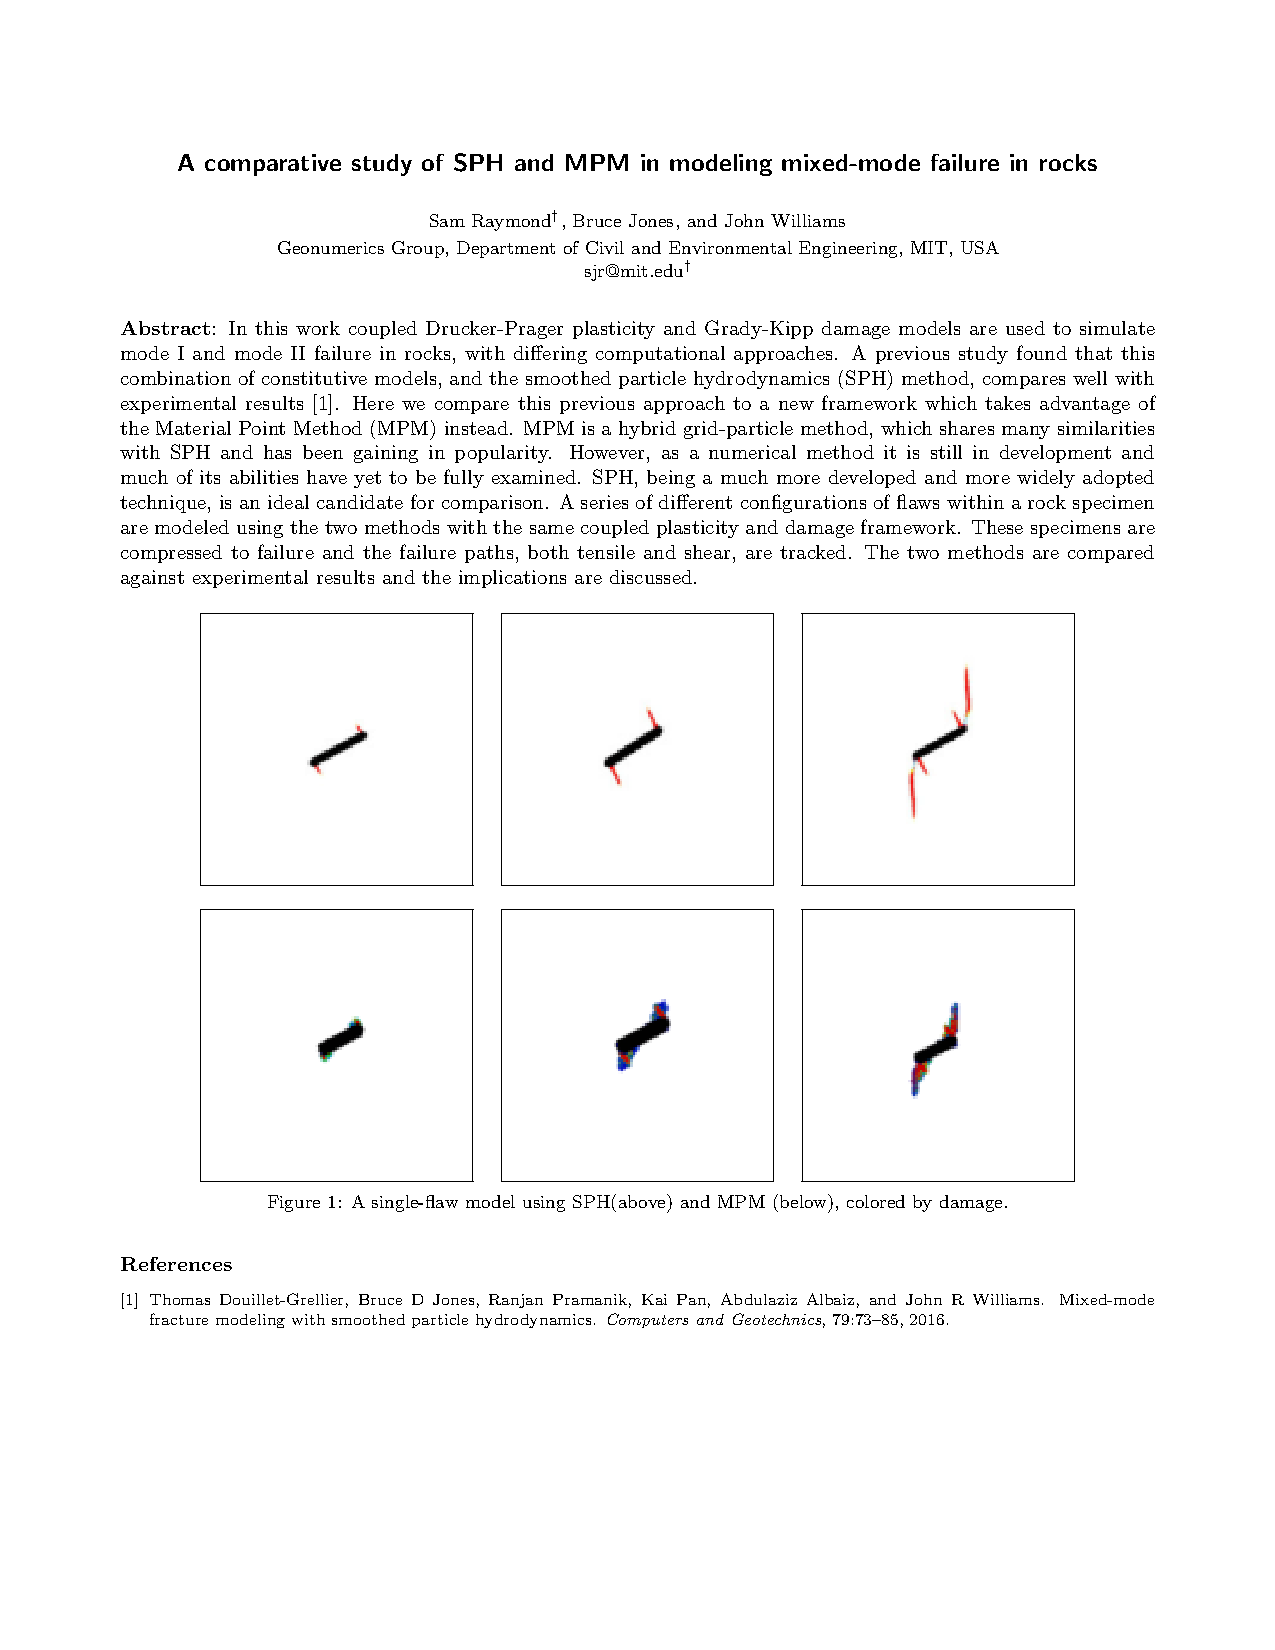
\includepdf[pages=-,pagecommand={\pagestyle{fancy}\label{5.1}},addtotoc={
     1,section,1,{~~~~~~~~Geotechnical Applications},p1,   
     1,subsection,1,A comparative study of SPH and MPM in modeling mixed-mode failure in rocks,p1}]{abstract/pdfs/4.pdf}
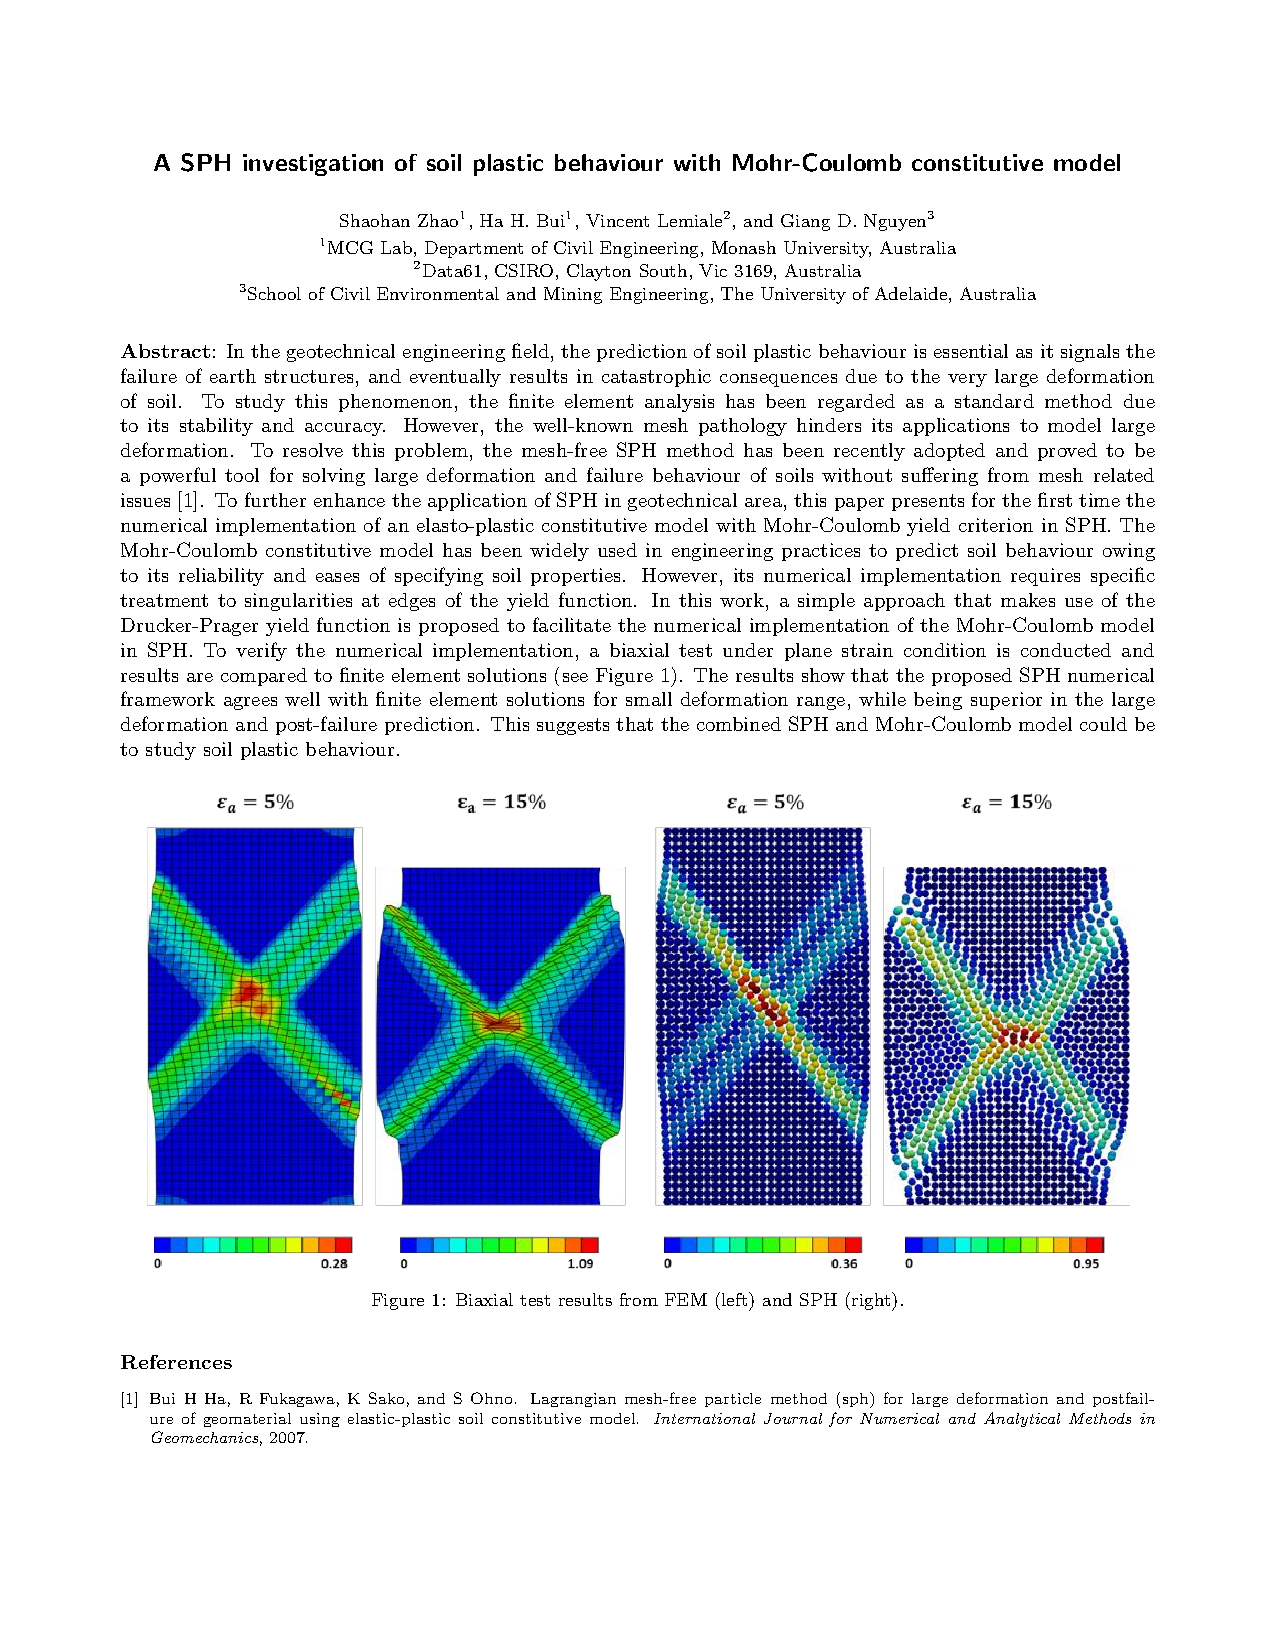
\includepdf[pages=-,pagecommand={\pagestyle{fancy}\label{5.2}},addtotoc={  
     1,subsection,1,A SPH investigation of soil plastic behaviour with Mohr-Coulomb constitutive model,p1}]{abstract/pdfs/5.pdf}
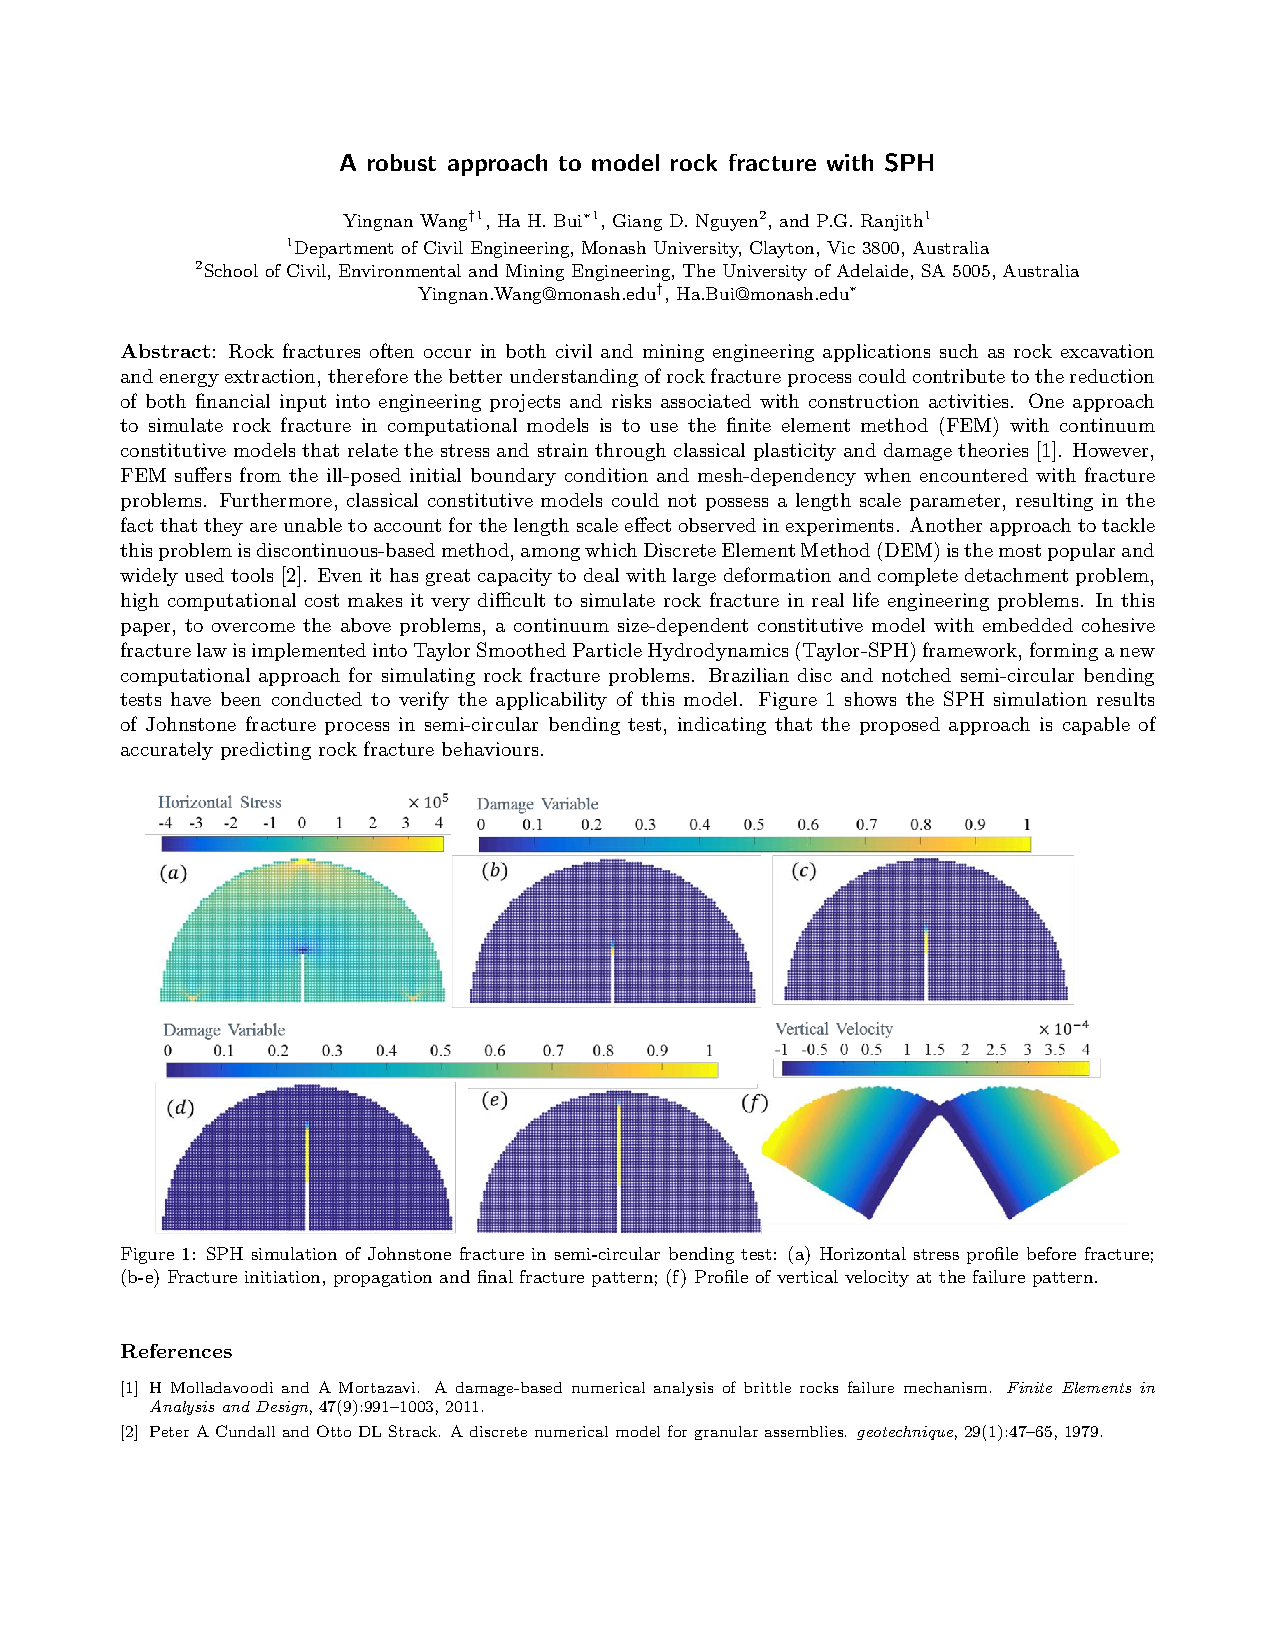
\includepdf[pages=-,pagecommand={\pagestyle{fancy}\label{5.3}},addtotoc={  
     1,subsection,1,A robust approach to model rock fracture with SPH,p1}]{abstract/pdfs/6.pdf}
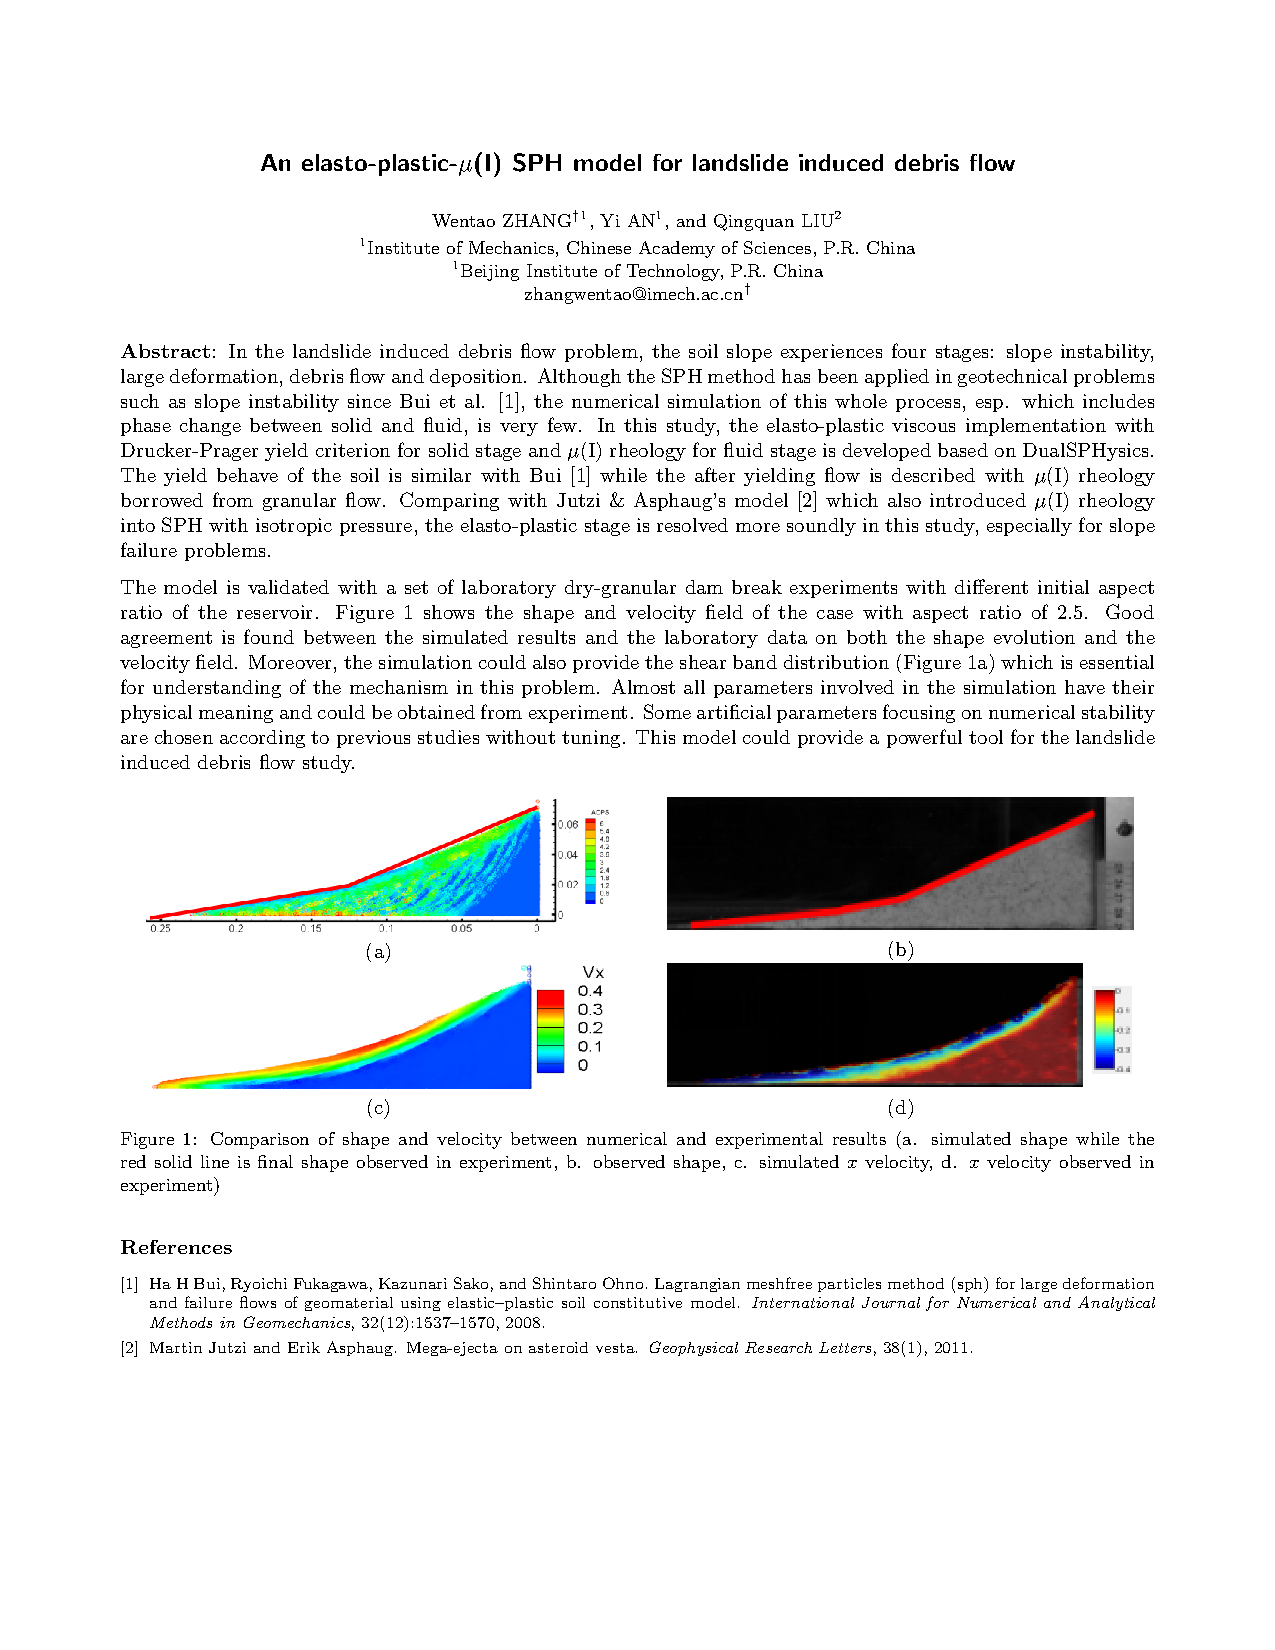
\includepdf[pages=-,pagecommand={\pagestyle{fancy}\label{5.4}},addtotoc={  
     1,subsection,1,An elasto-plastic-$\mu$(I) SPH model for landslide induced debris flow,p1}]{abstract/pdfs/33.pdf}



%\section{Session 6: Hydraulic Applications I}
%6.1: 10
%6.2: 48
%6.3: 46
%6.4: 55


\rhead{Session 6}
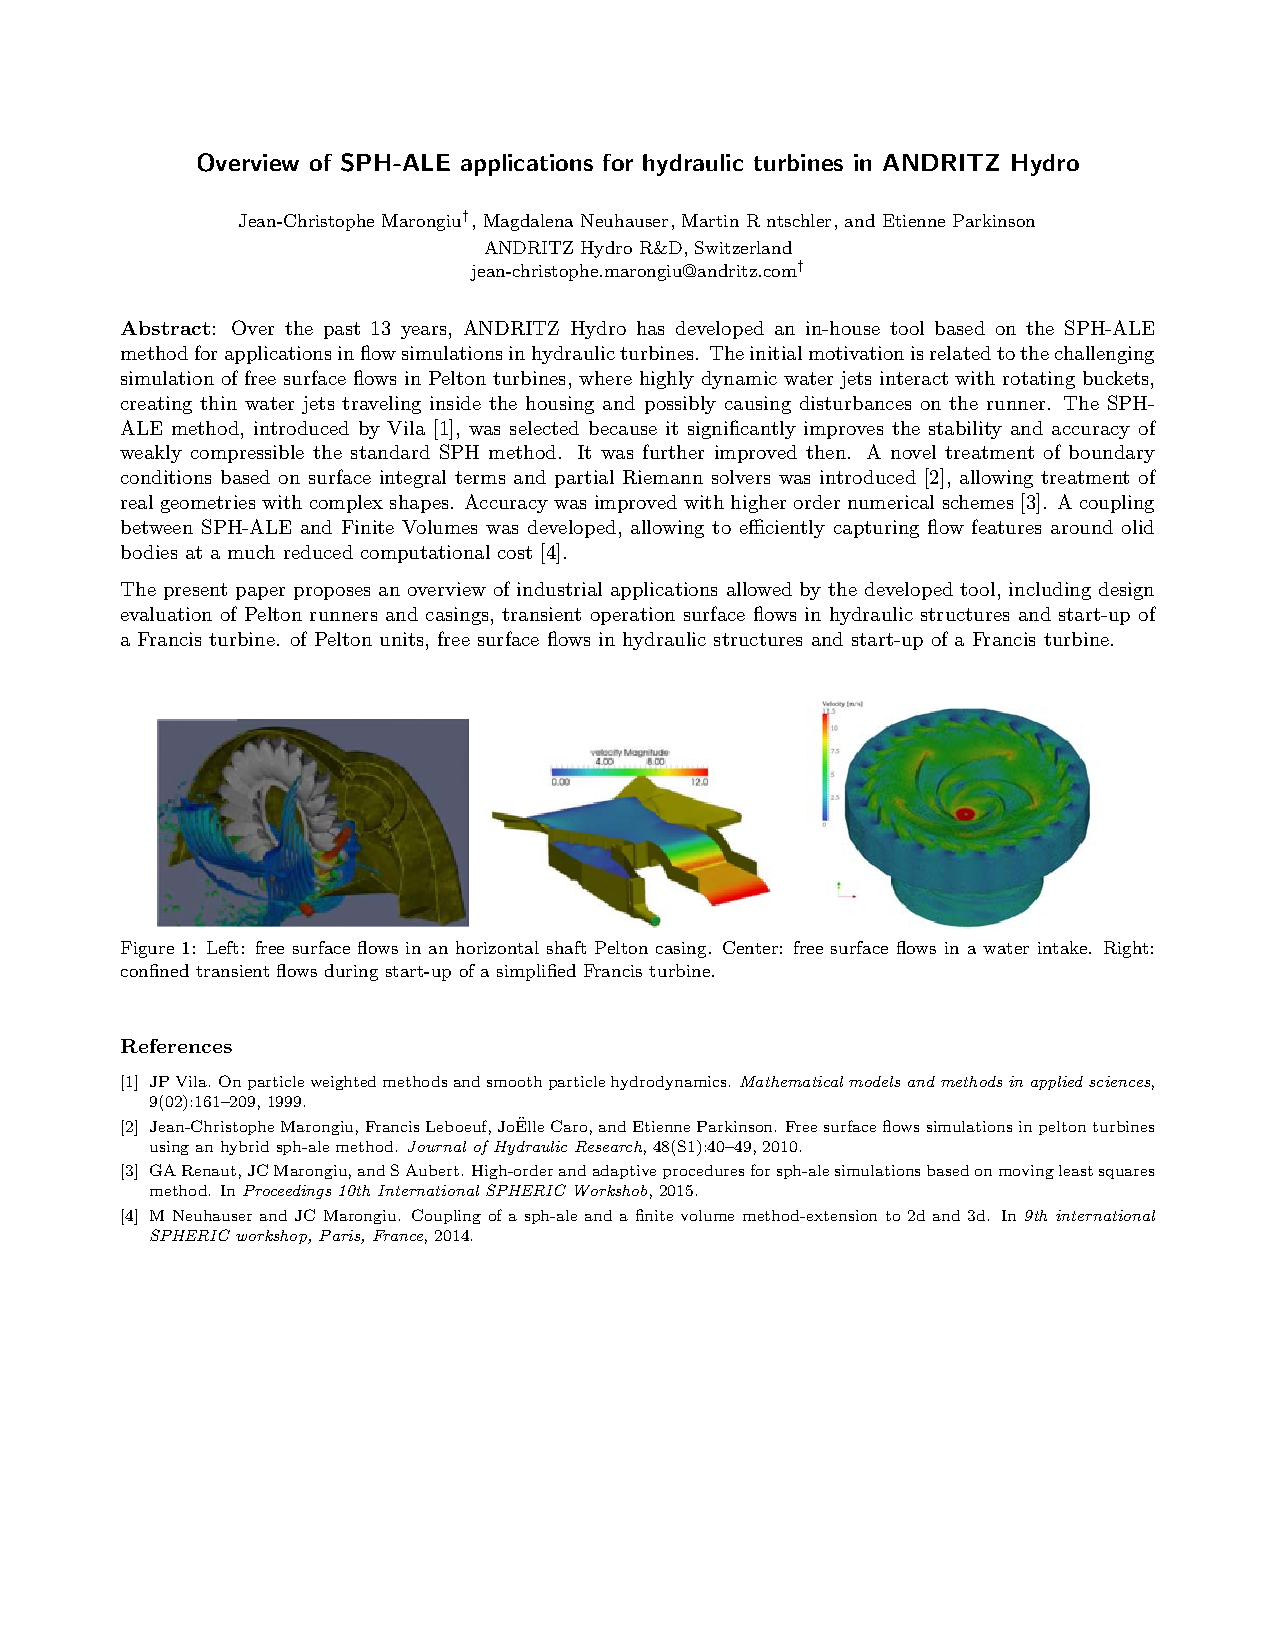
\includepdf[pages=-,pagecommand={\pagestyle{fancy}\label{6.1}},addtotoc={
     1,section,1,{~~~~~~~~Hydraulic Applications I},p1,   
     1,subsection,1,Overview of SPH-ALE applications for hydraulic turbines in ANDRITZ Hydro,p1}]{abstract/pdfs/10.pdf}
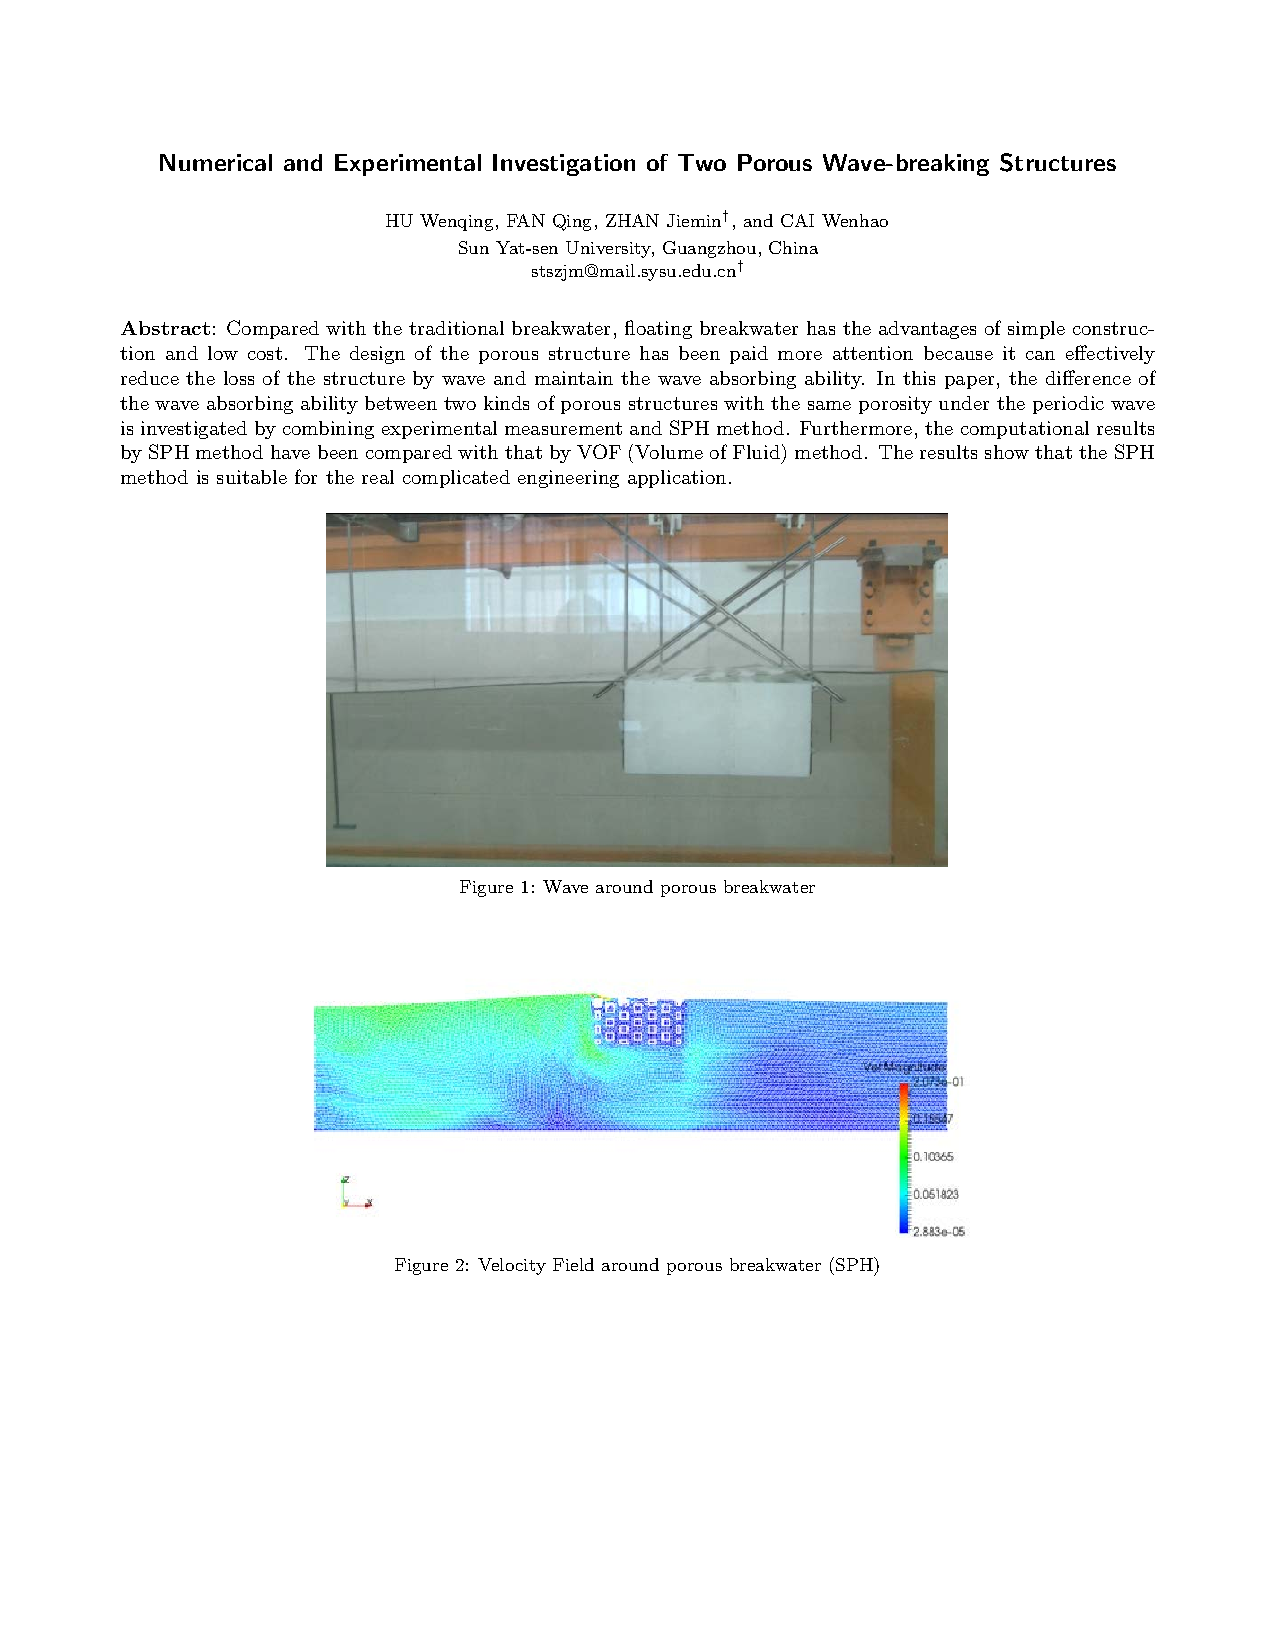
\includepdf[pages=-,pagecommand={\pagestyle{fancy}\label{6.2}},addtotoc={  
     1,subsection,1,Numerical and experimental investigation of two porous wave-breaking structures,p1}]{abstract/pdfs/48.pdf}
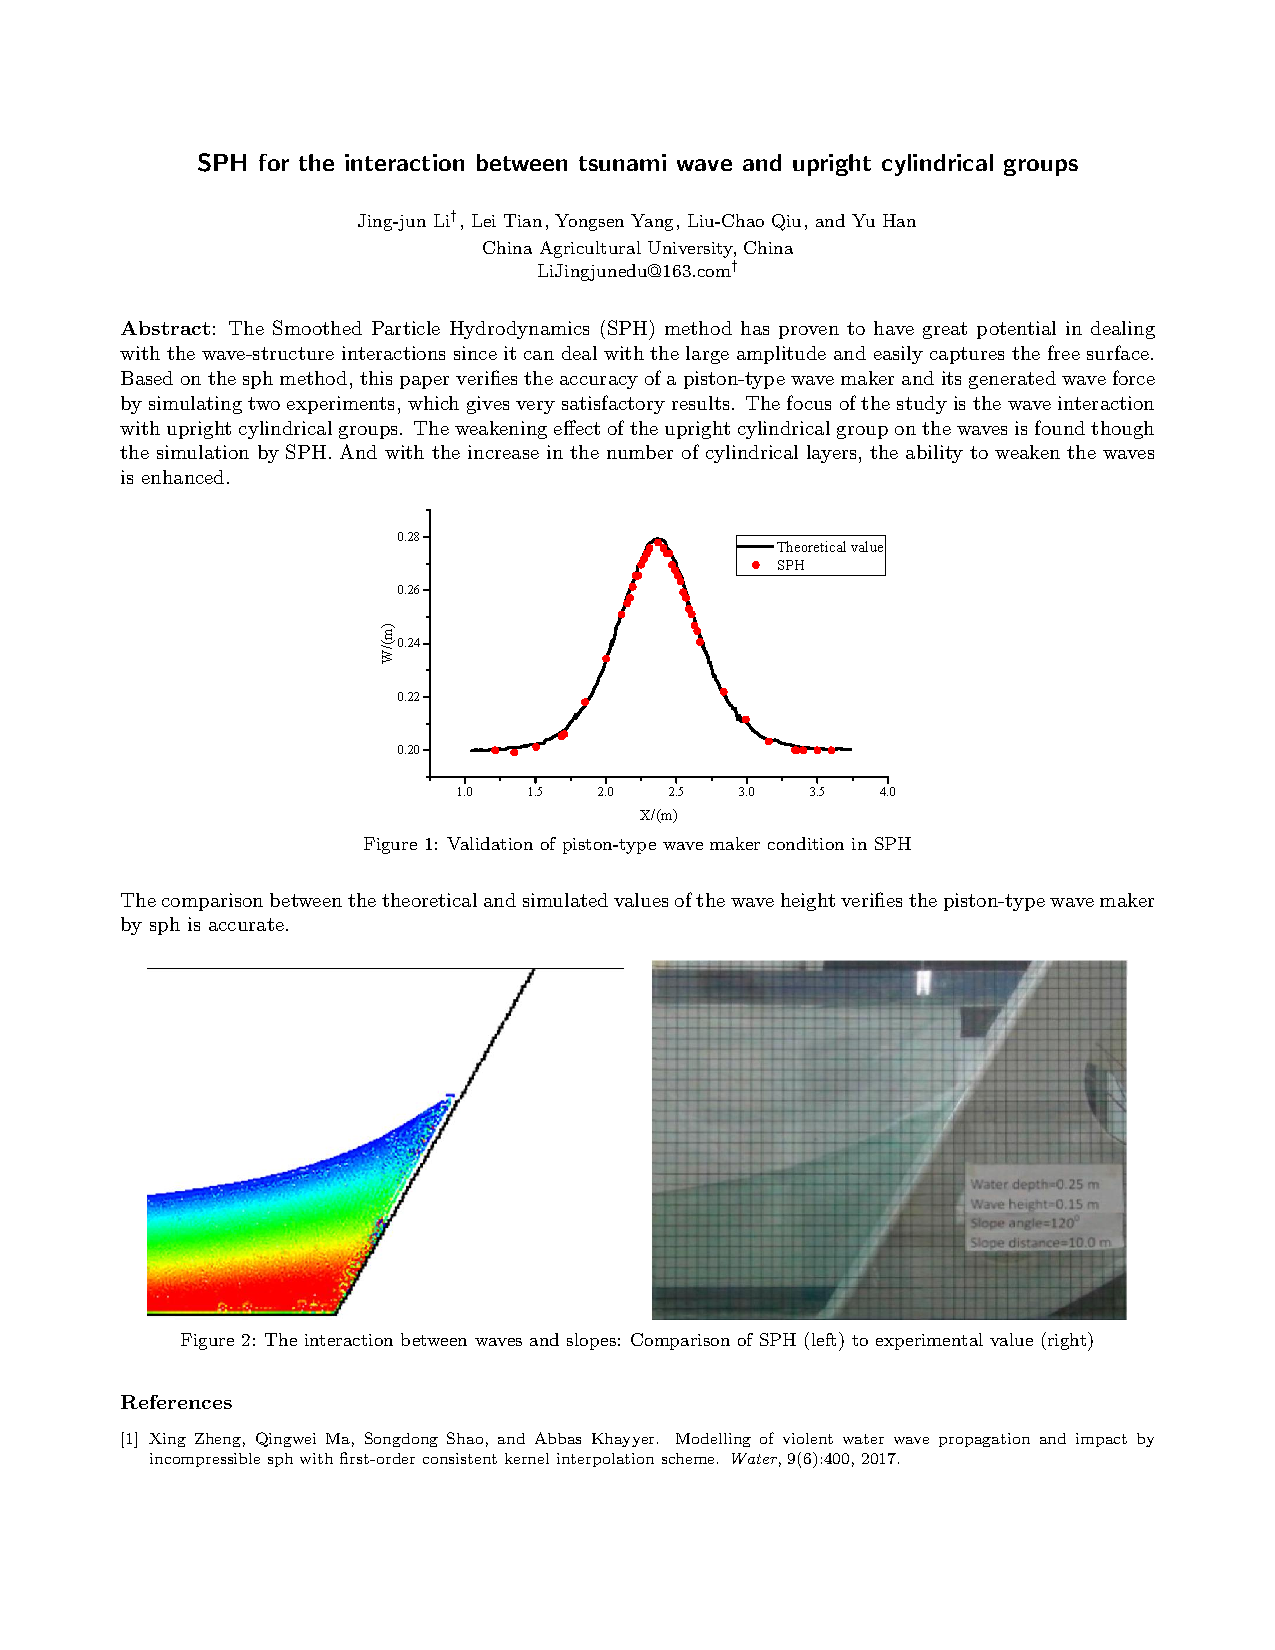
\includepdf[pages=-,pagecommand={\pagestyle{fancy}\label{6.3}},addtotoc={  
     1,subsection,1,SPH for the interaction between tsunami wave and upright cylindrical groups,p1}]{abstract/pdfs/46.pdf}
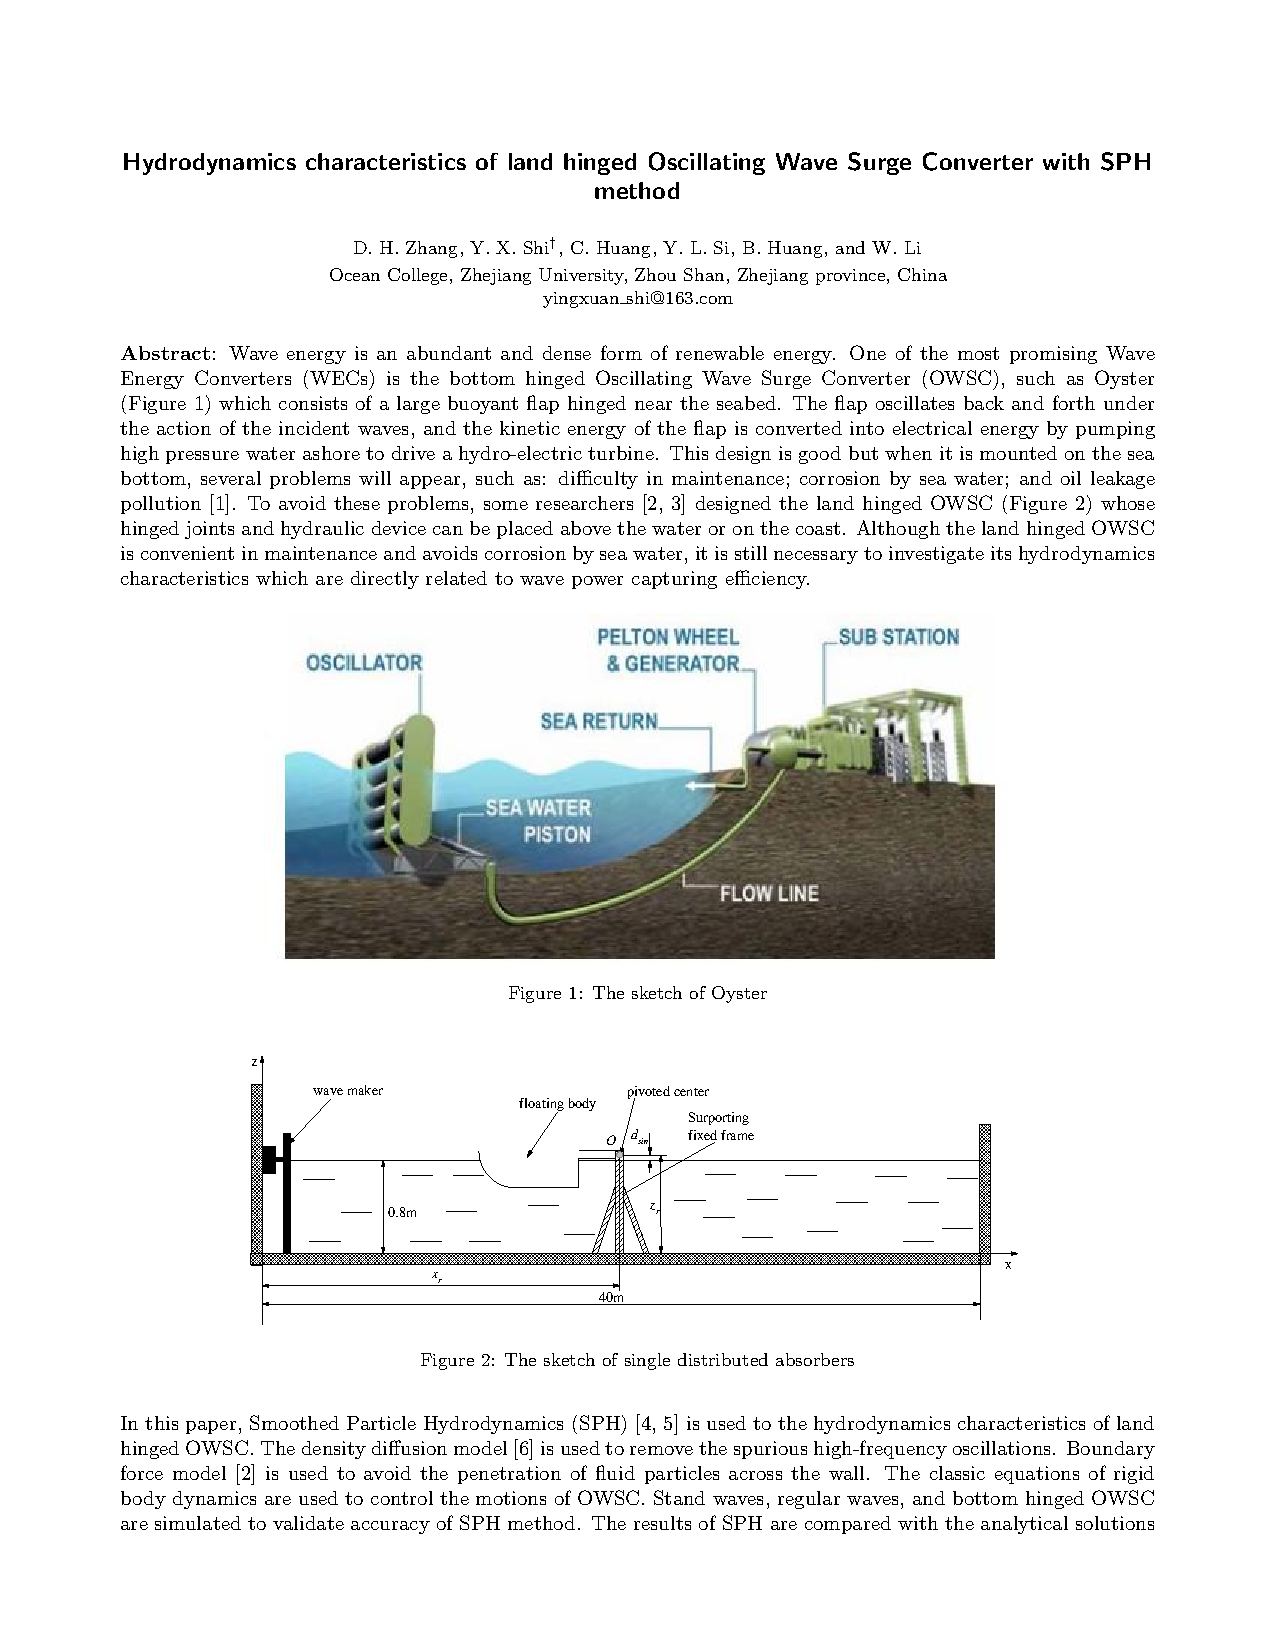
\includepdf[pages=-,pagecommand={\pagestyle{fancy}\label{6.4}},addtotoc={  
     1,subsection,1,Hydrodynamics characteristics of land hinged oscillating wave surge converter with SPH method,p1}]{abstract/pdfs/55.pdf}


%\section{Session 7: Adaptivity (variable resolution)}
%7.1: 15
%7.2: 29
%7.3: 12

\rhead{Session 7}
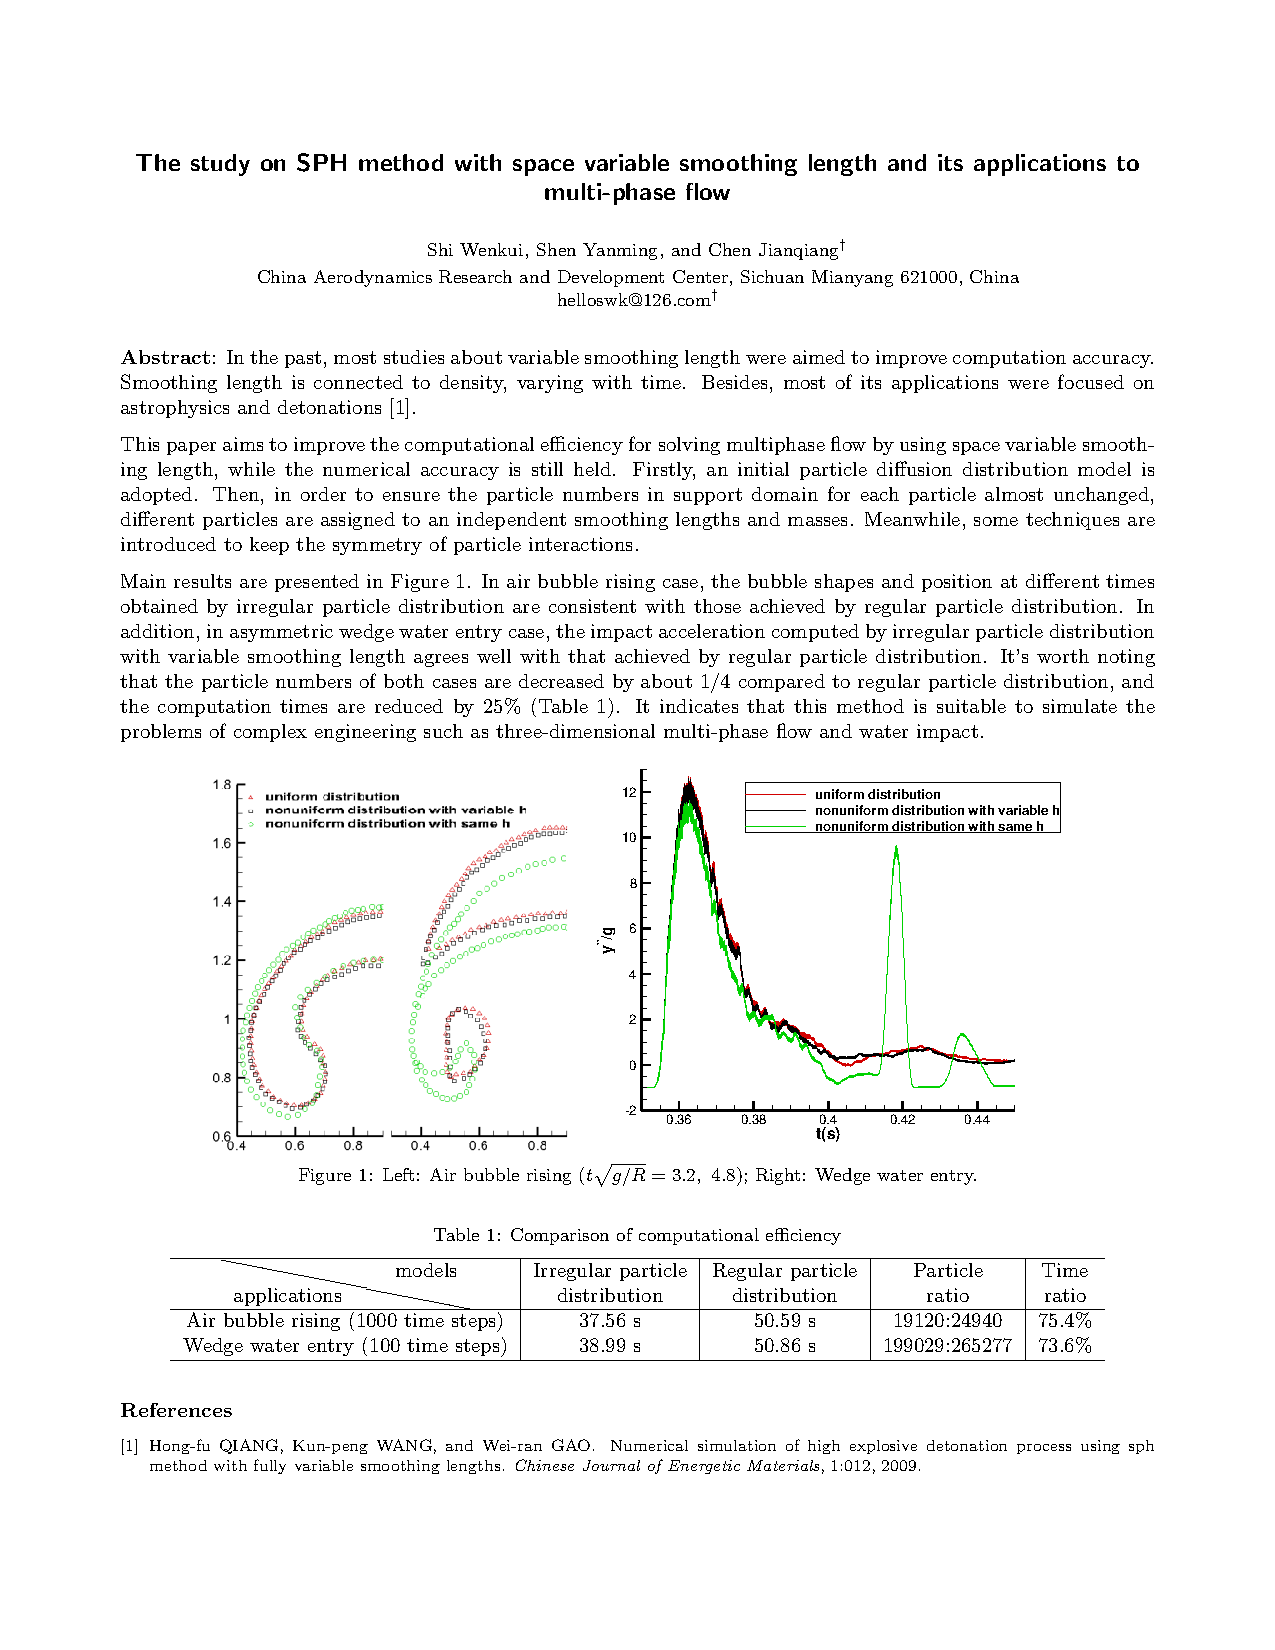
\includepdf[pages=-,pagecommand={\pagestyle{fancy}\label{7.1}},addtotoc={
     1,section,1,{~~~~~~~~Adaptivity (variable resolution)},p1,   
     1,subsection,1,The study on SPH method with space variable smoothing length and its applications to multi-phase flow,p1}]{abstract/pdfs/15.pdf}
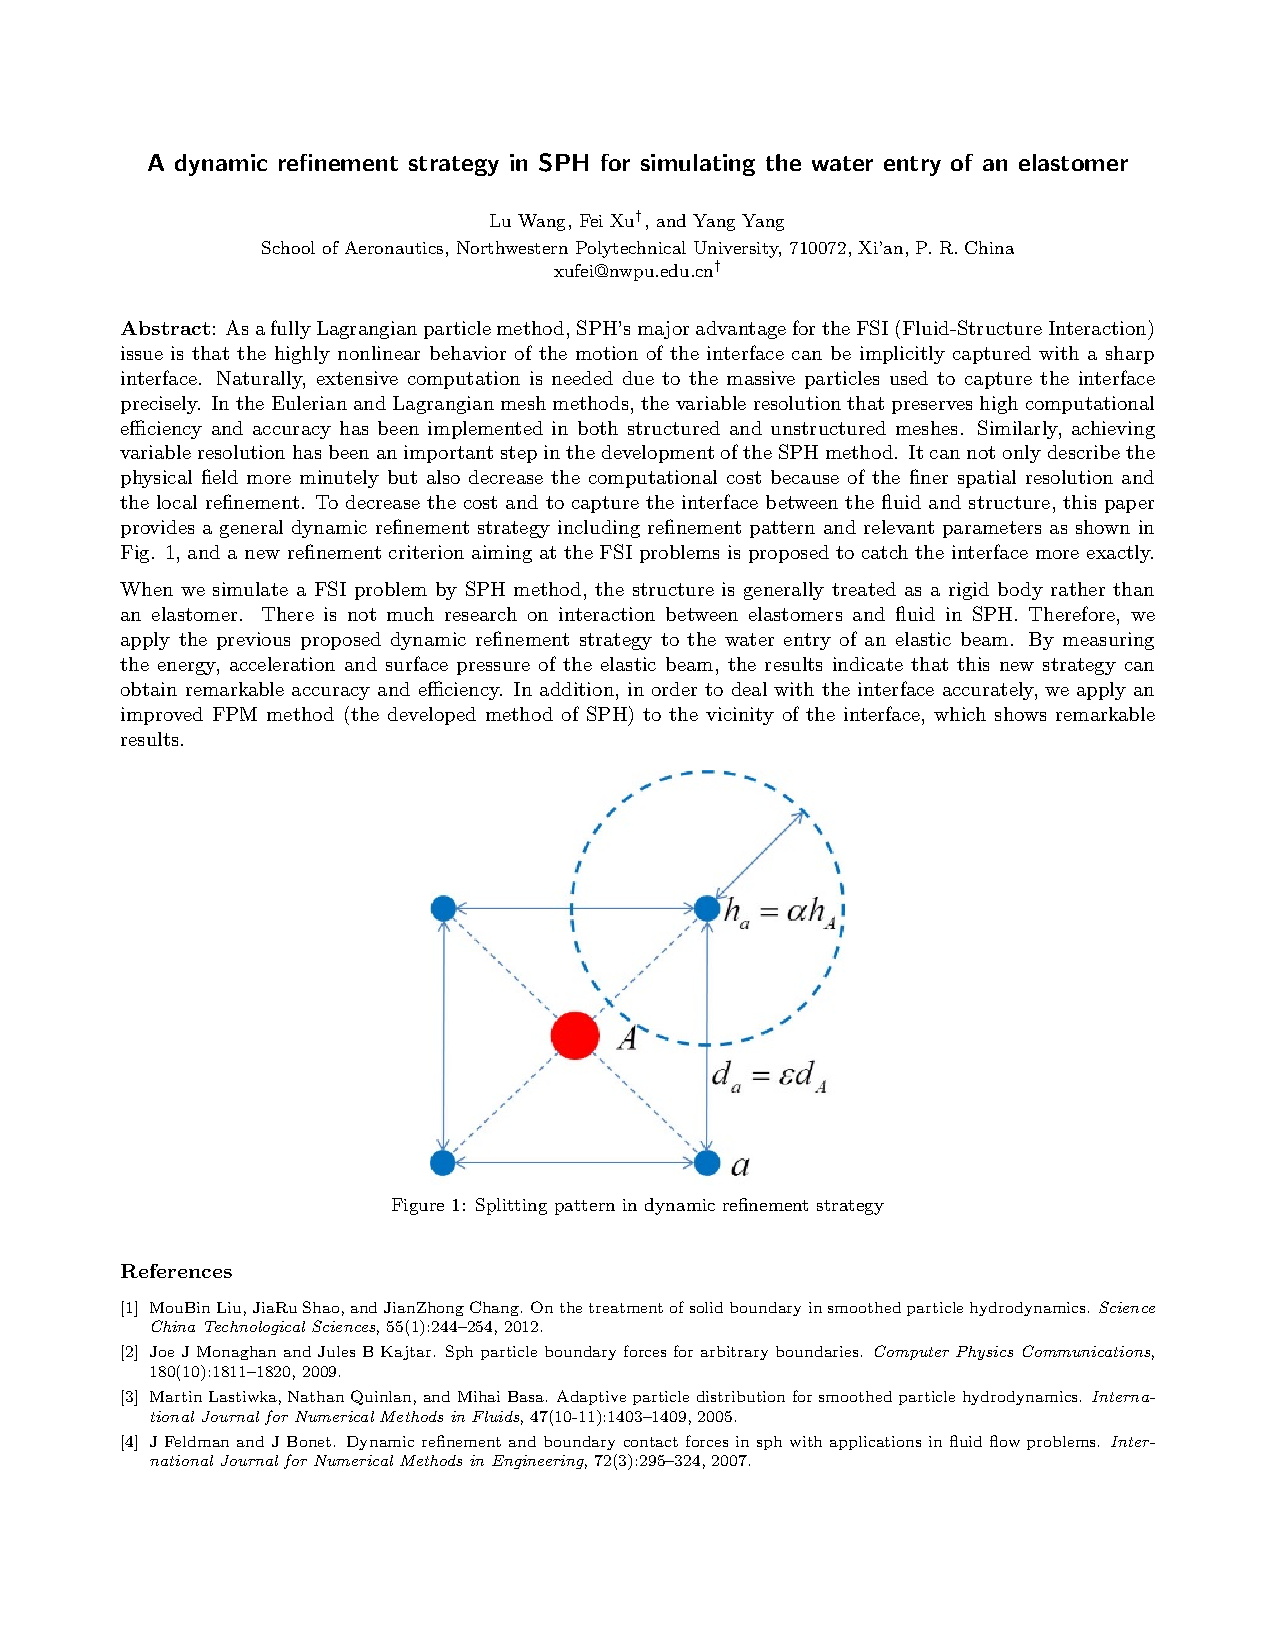
\includepdf[pages=-,pagecommand={\pagestyle{fancy}\label{7.2}},addtotoc={  
     1,subsection,1,A dynamic refinement strategy in SPH for simulating the water entry of an elastomer,p1}]{abstract/pdfs/29.pdf}
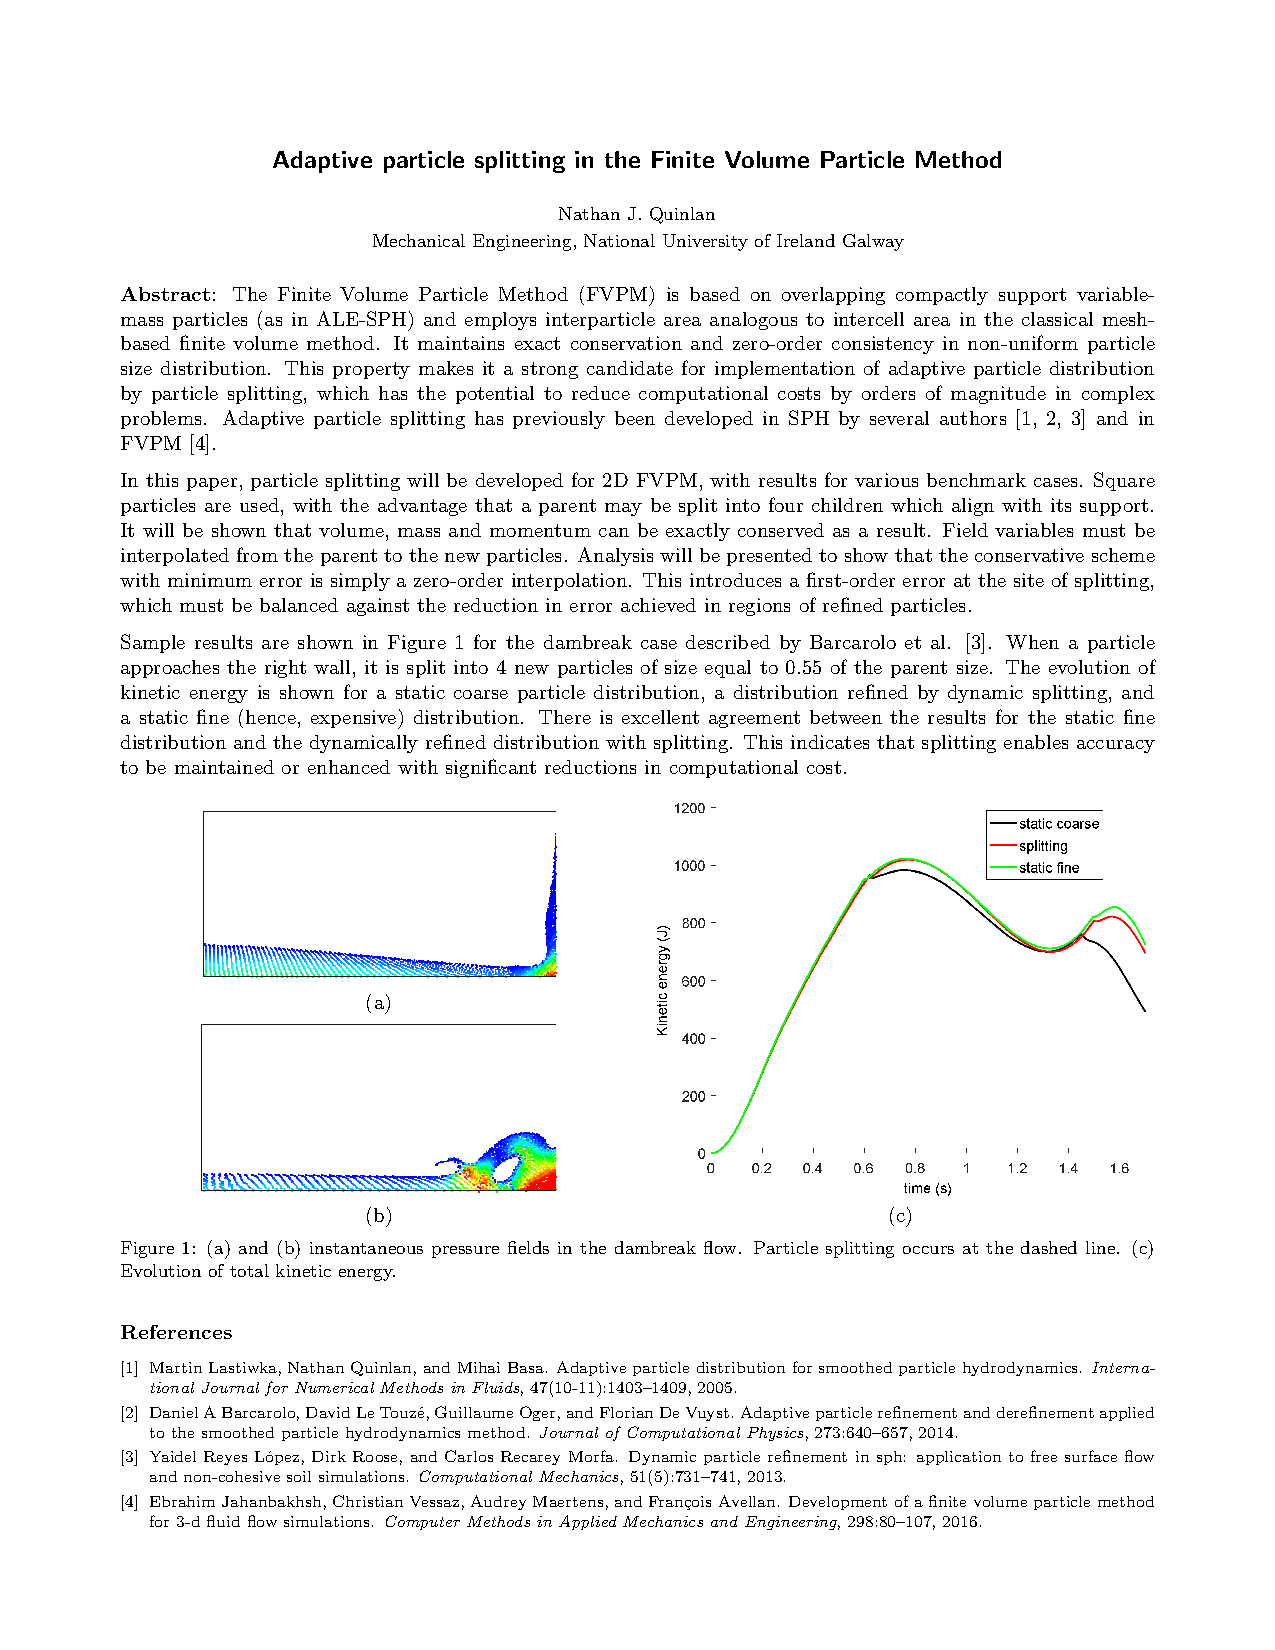
\includepdf[pages=-,pagecommand={\pagestyle{fancy}\label{7.3}},addtotoc={  
     1,subsection,1,Adaptive particle splitting in the finite volume particle method,p1}]{abstract/pdfs/12.pdf}



%\section{Session 8: New applications of SPH}
%8.1: 25
%8.2: 38
%8.3: 3
%8.4: 9

\rhead{Session 8}
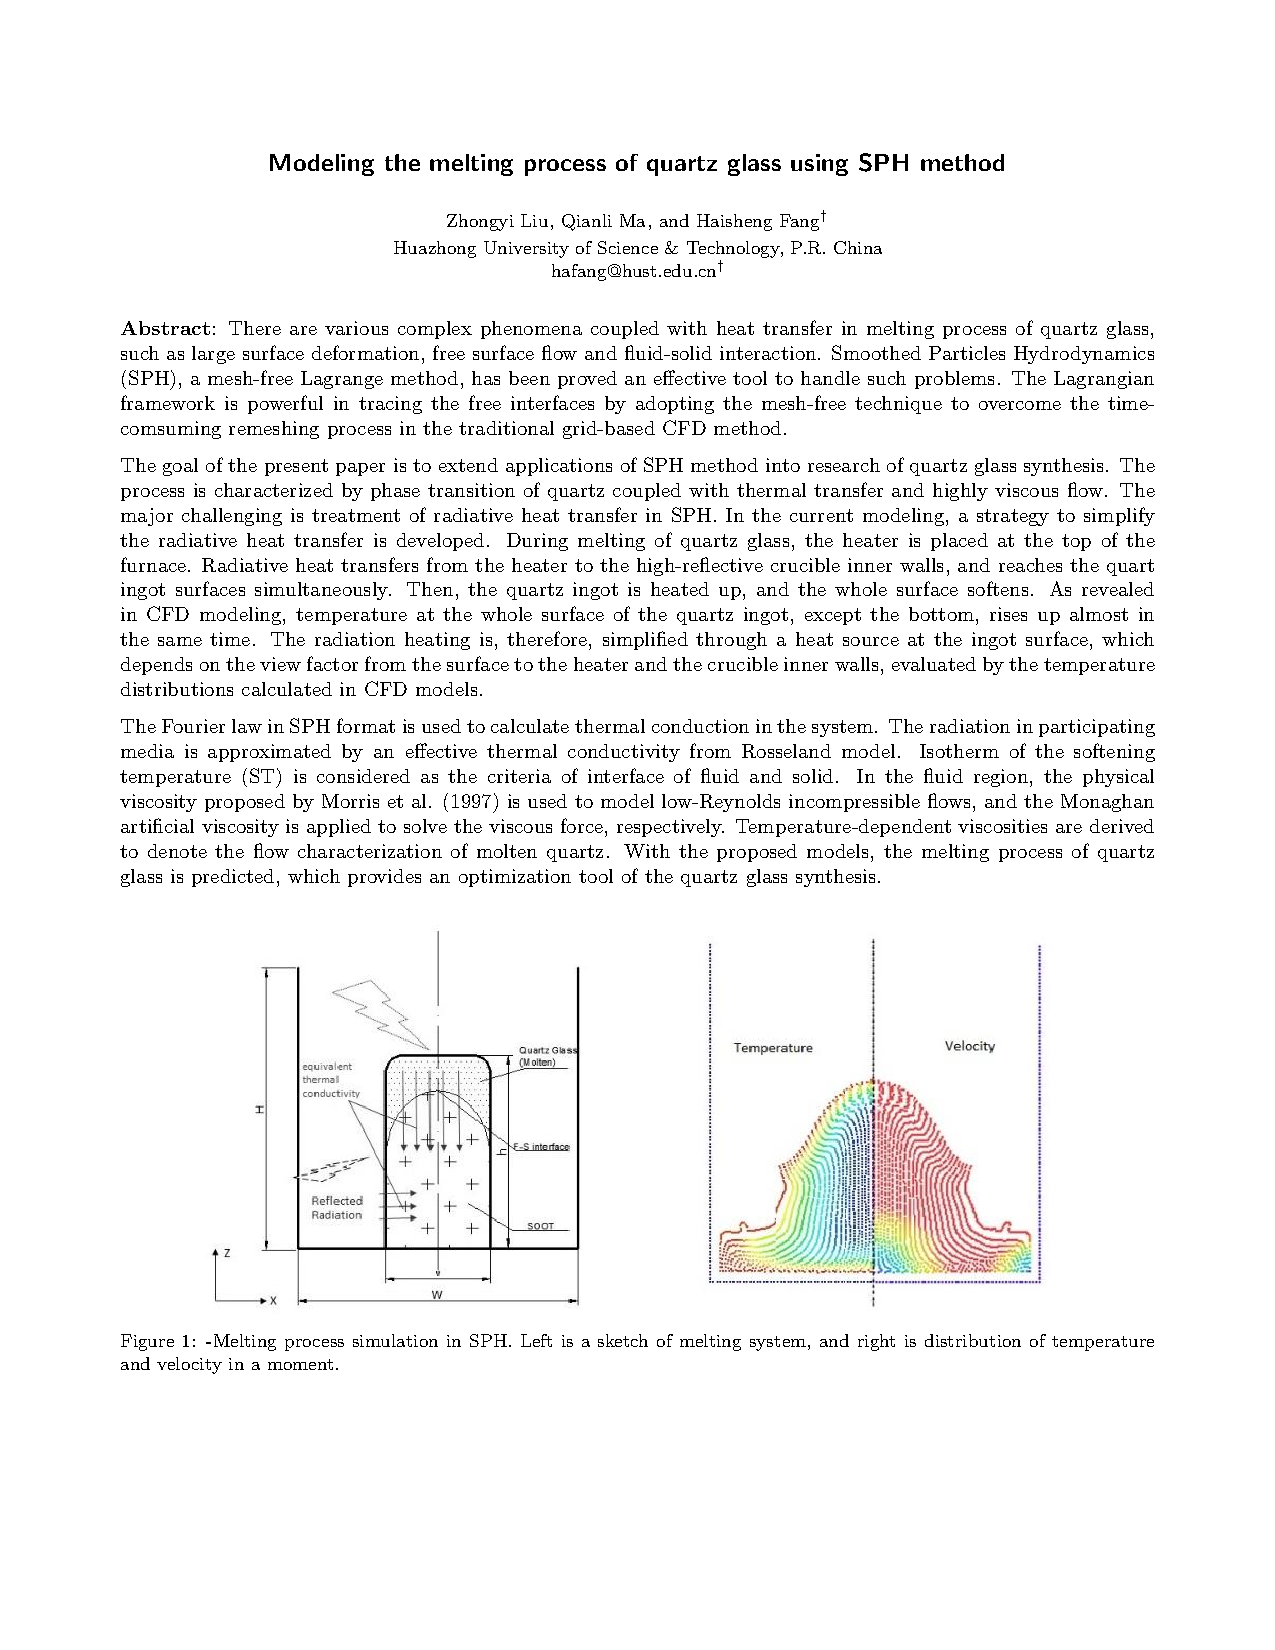
\includepdf[pages=-,pagecommand={\pagestyle{fancy}\label{8.1}},addtotoc={
     1,section,1,{~~~~~~~~New applications of SPH},p1,   
     1,subsection,1,Modeling the melting process of quartz glass using SPH method,p1}]{abstract/pdfs/25.pdf}
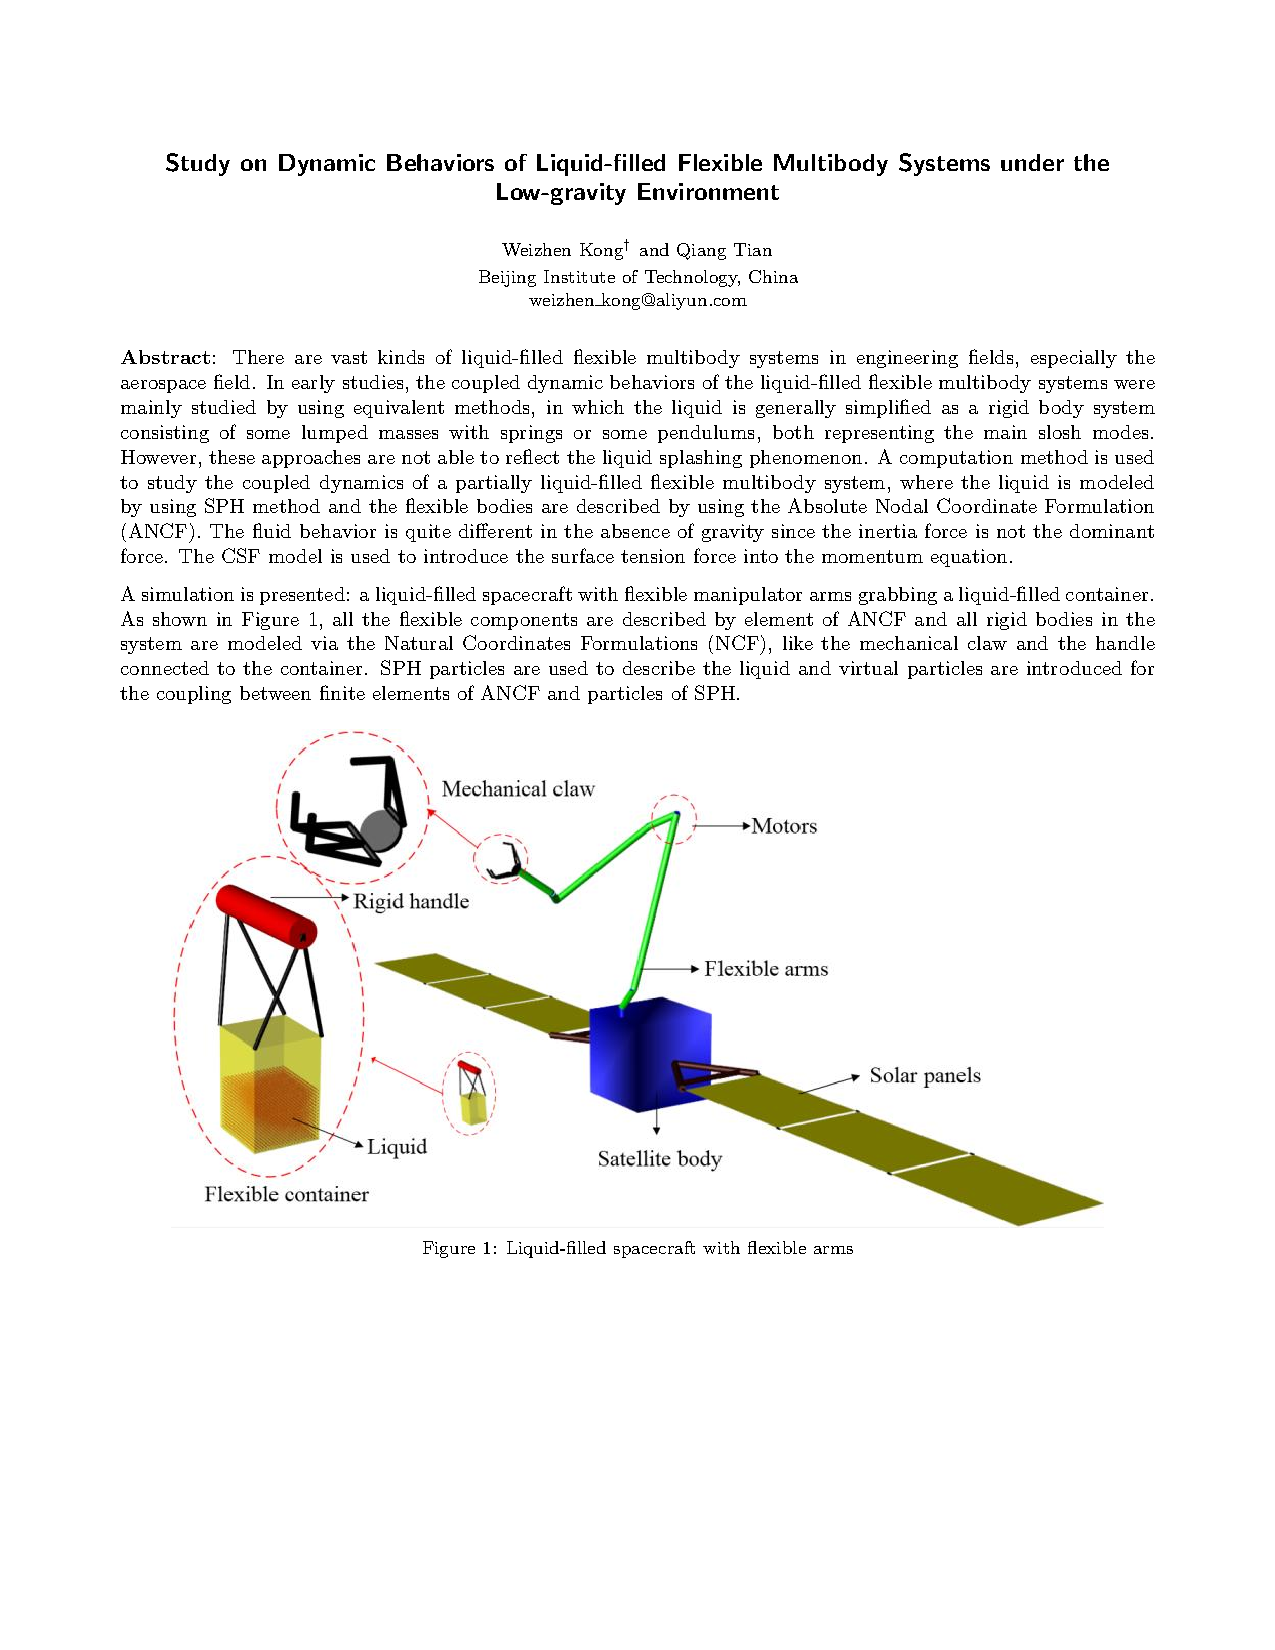
\includepdf[pages=-,pagecommand={\pagestyle{fancy}\label{8.2}},addtotoc={  
     1,subsection,1,Study on dynamic behaviors of liquid-filled flexible multibody systems under the low-gravity environment,p1}]{abstract/pdfs/38.pdf}
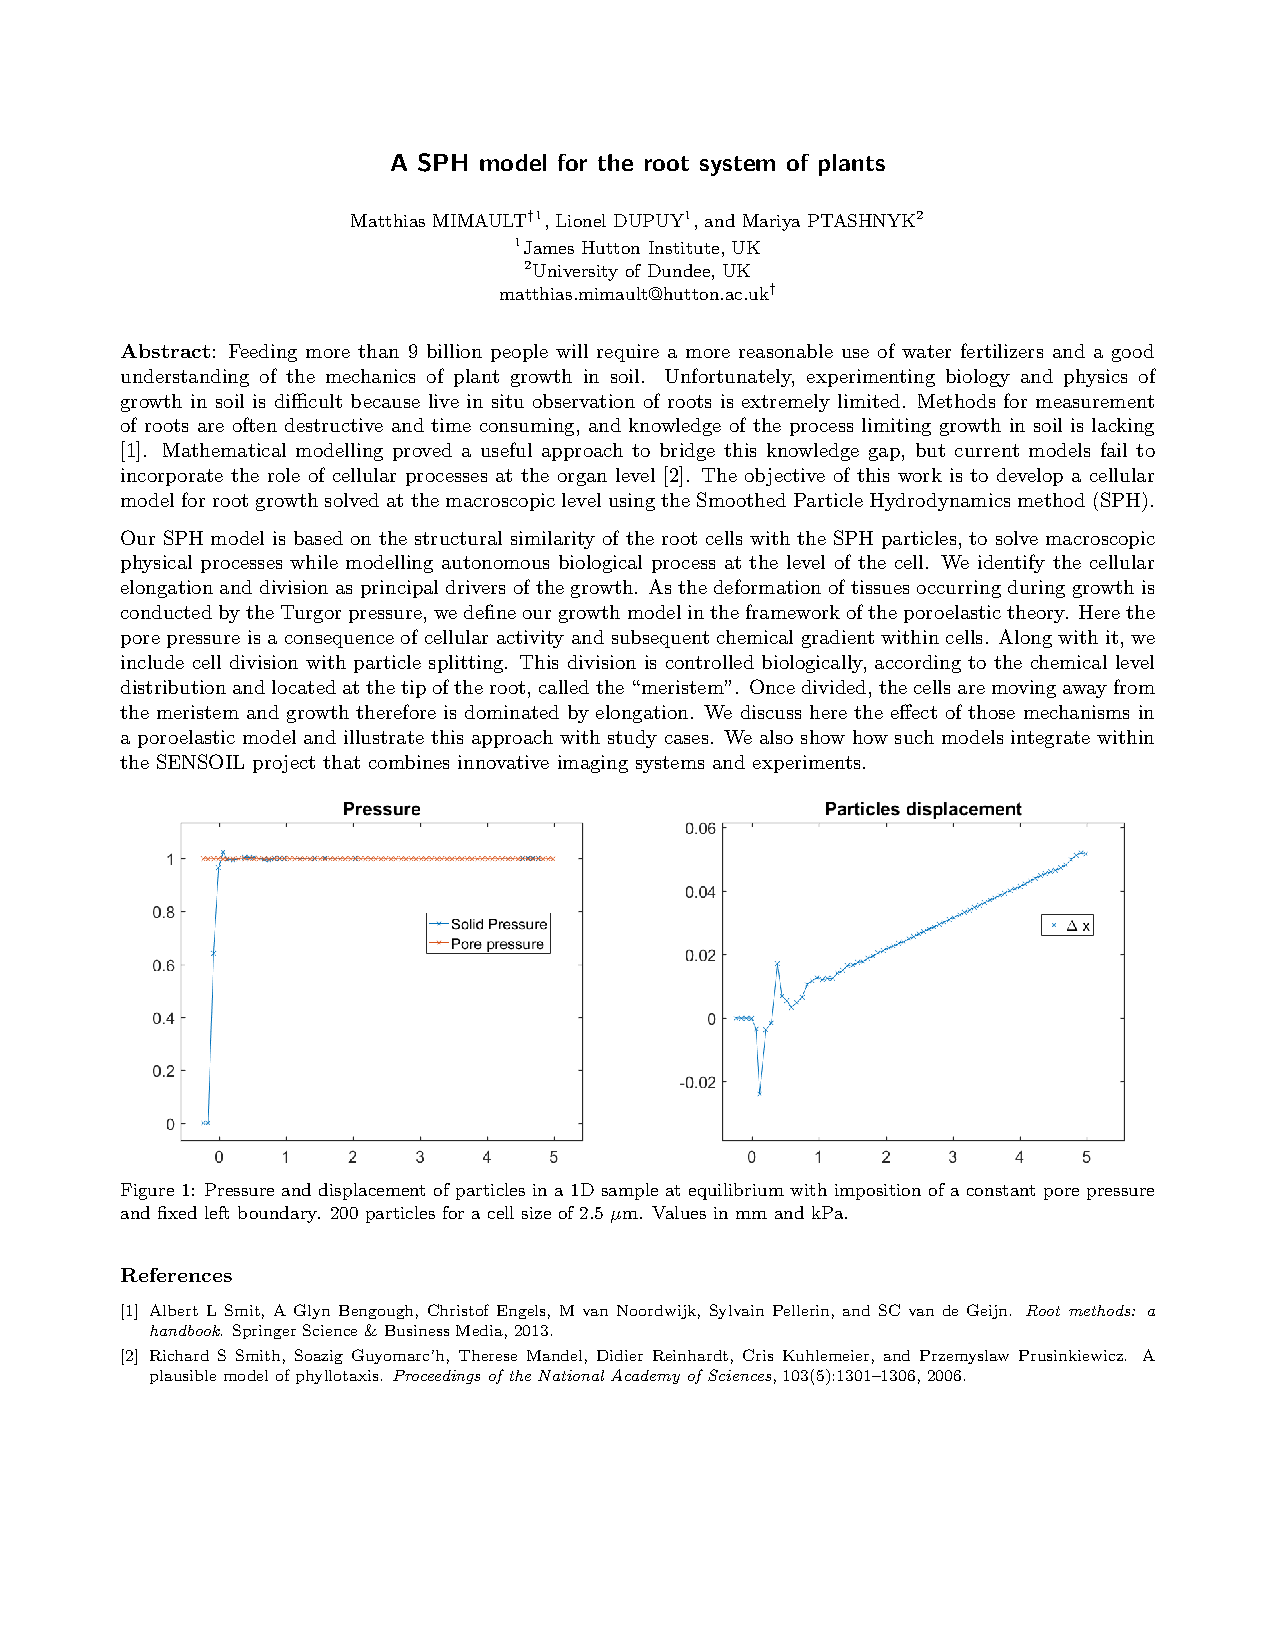
\includepdf[pages=-,pagecommand={\pagestyle{fancy}\label{8.3}},addtotoc={  
     1,subsection,1,A SPH model for the root system of plants,p1}]{abstract/pdfs/3.pdf}
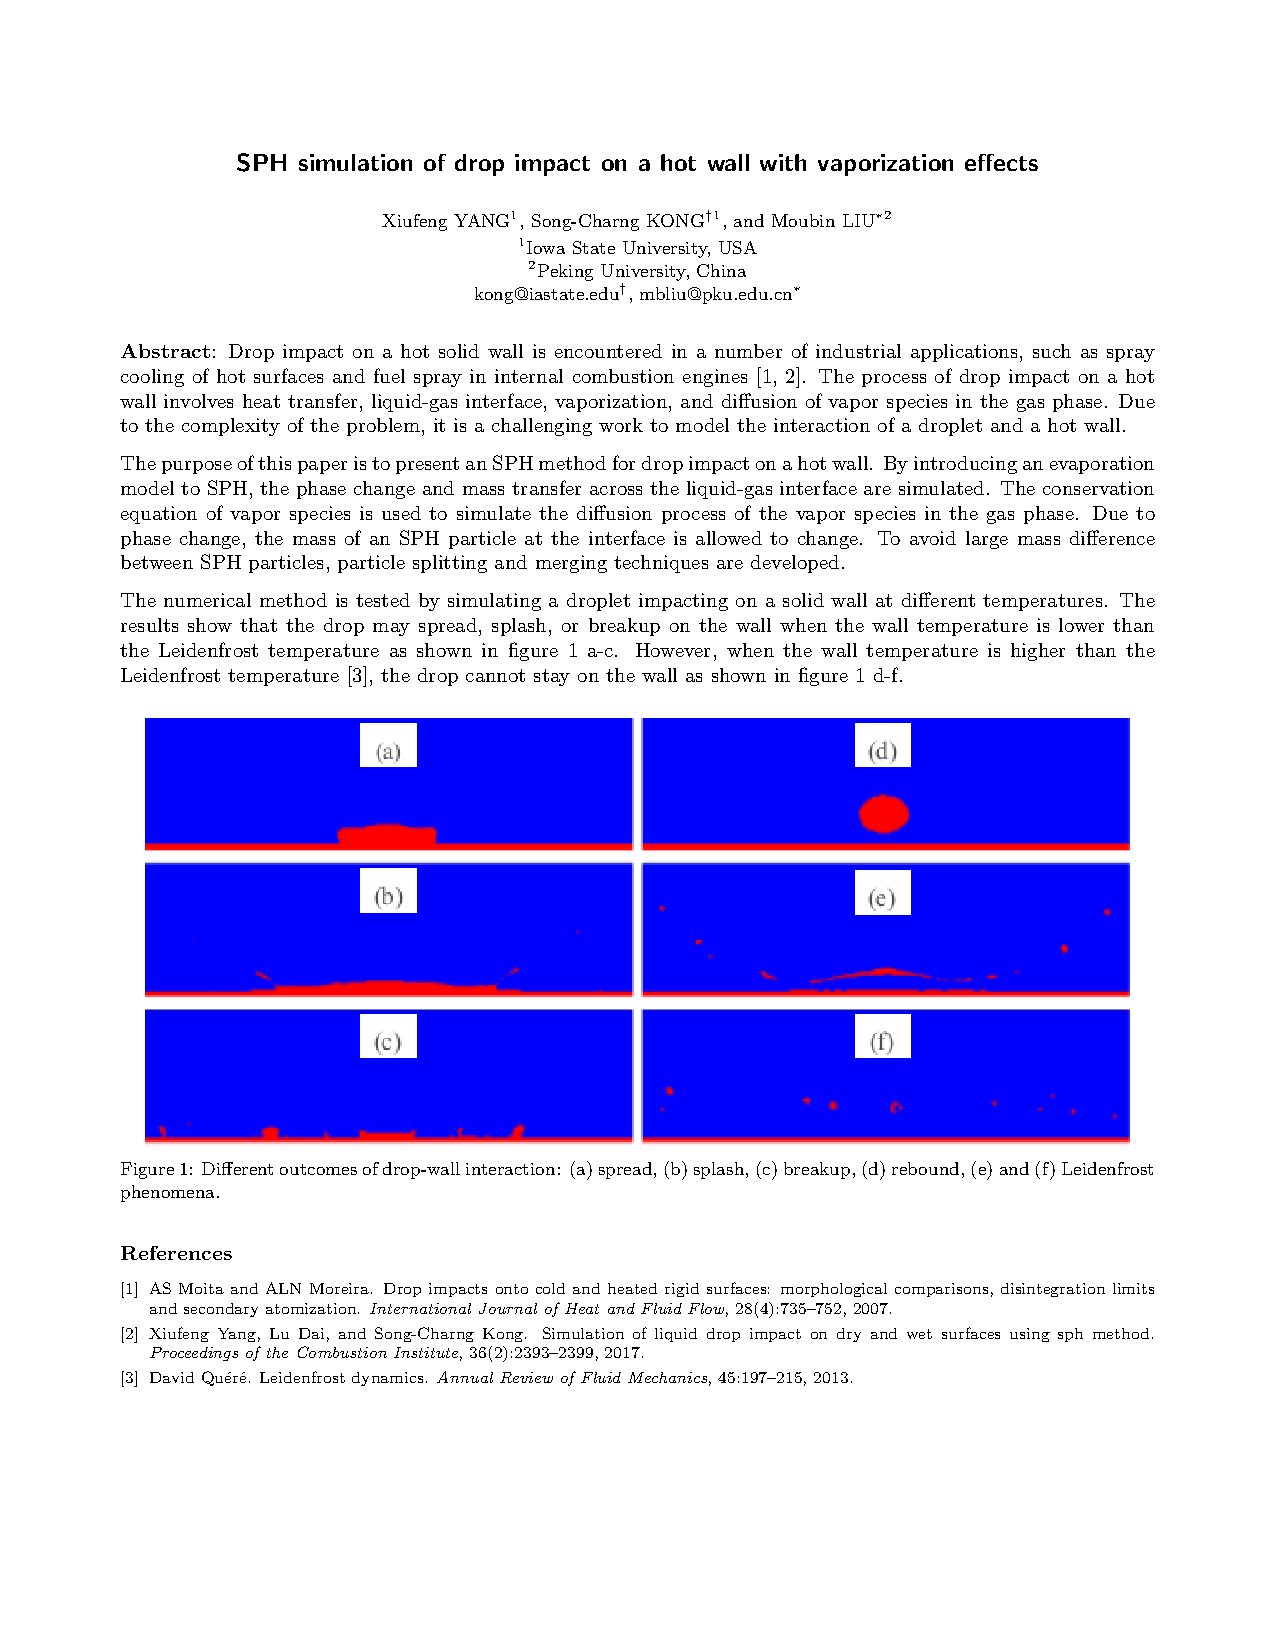
\includepdf[pages=-,pagecommand={\pagestyle{fancy}\label{8.4}},addtotoc={  
     1,subsection,1,SPH simulation of drop impact on a hot wall with vaporization effects,p1}]{abstract/pdfs/9.pdf}



%\section{Session 9: High-Performance Computing}
%9.1: 11
%9.2: 16
%9.3: 26
%9.4: ????????????????????????


\rhead{Session 9}
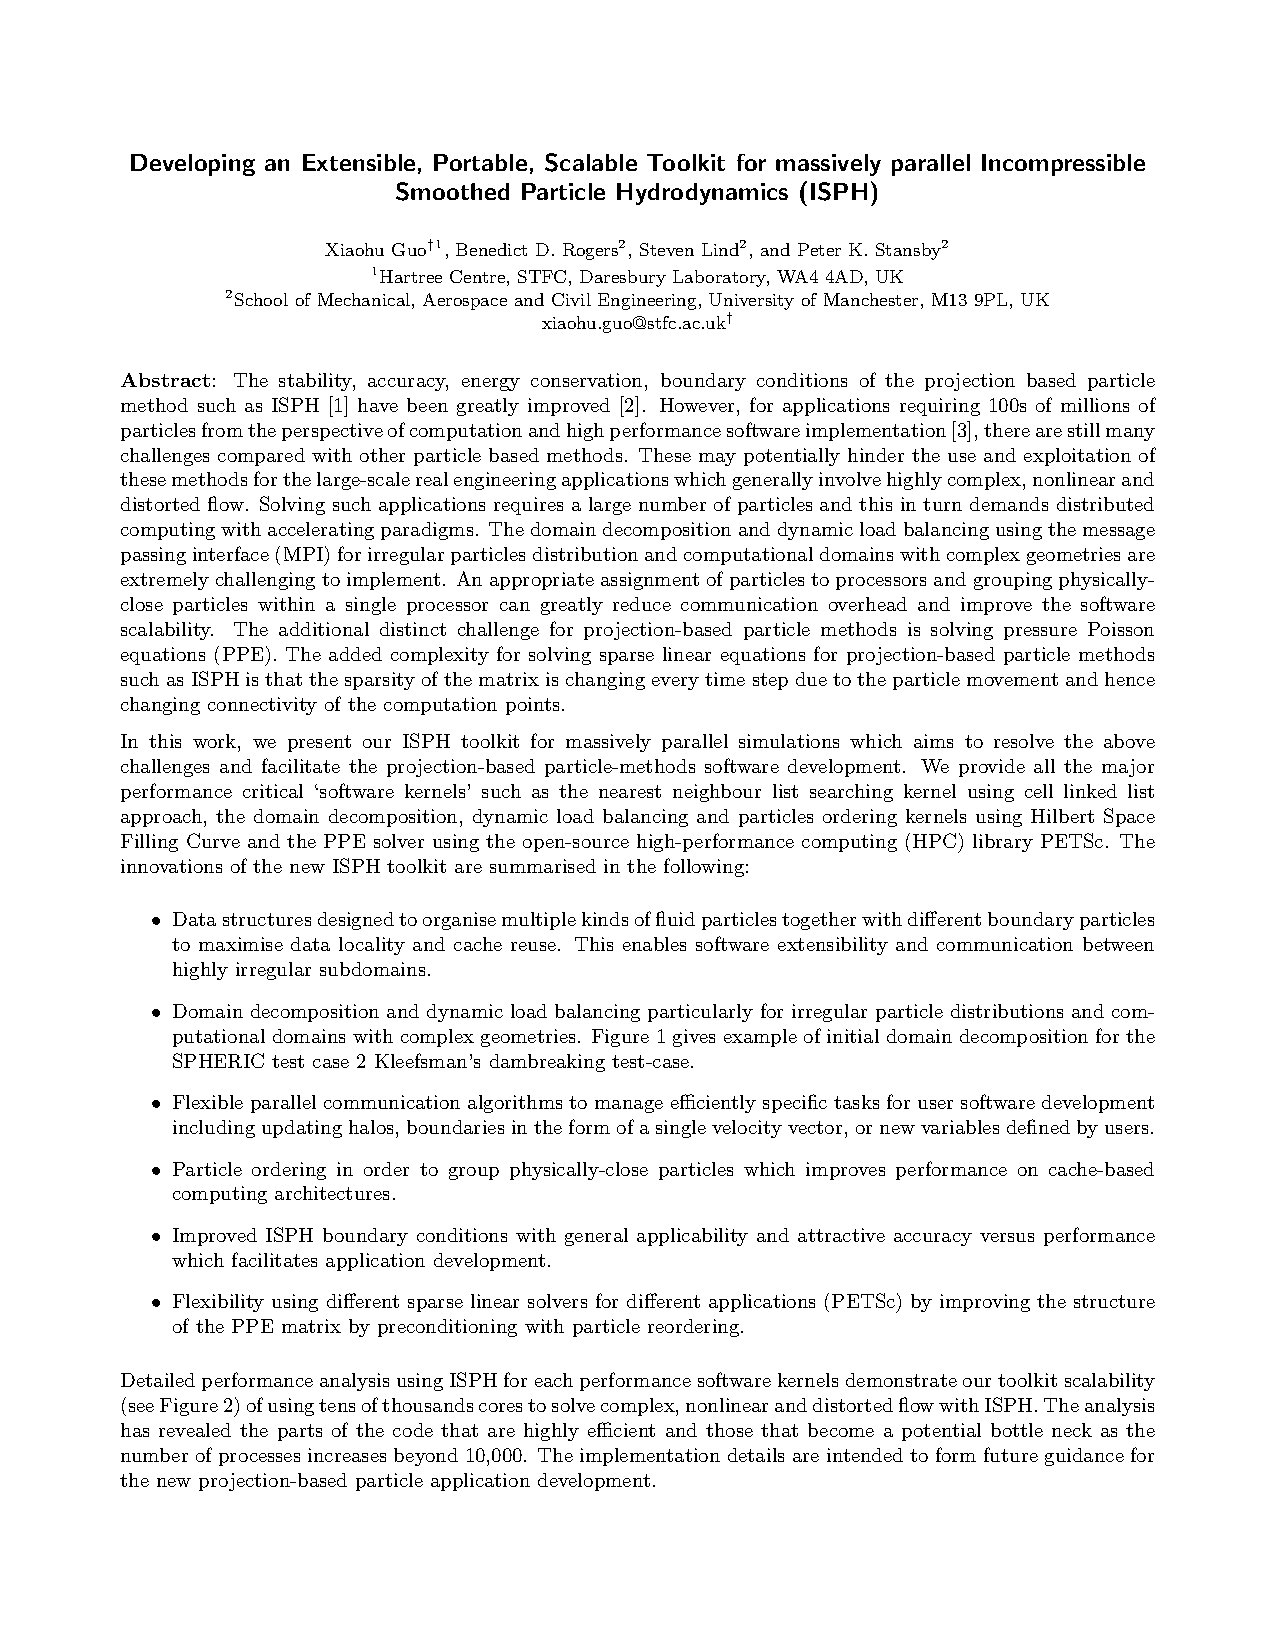
\includepdf[pages=-,pagecommand={\pagestyle{fancy}\label{9.1}},addtotoc={
     1,section,1,{~~~~~~~~High-Performance Computing},p1,   
     1,subsection,1,{Developing an extensible, portable, scalable toolkit for massively parallel incompressible smoothed particle hydrodynamics (ISPH)},p1}]{abstract/pdfs/11.pdf}
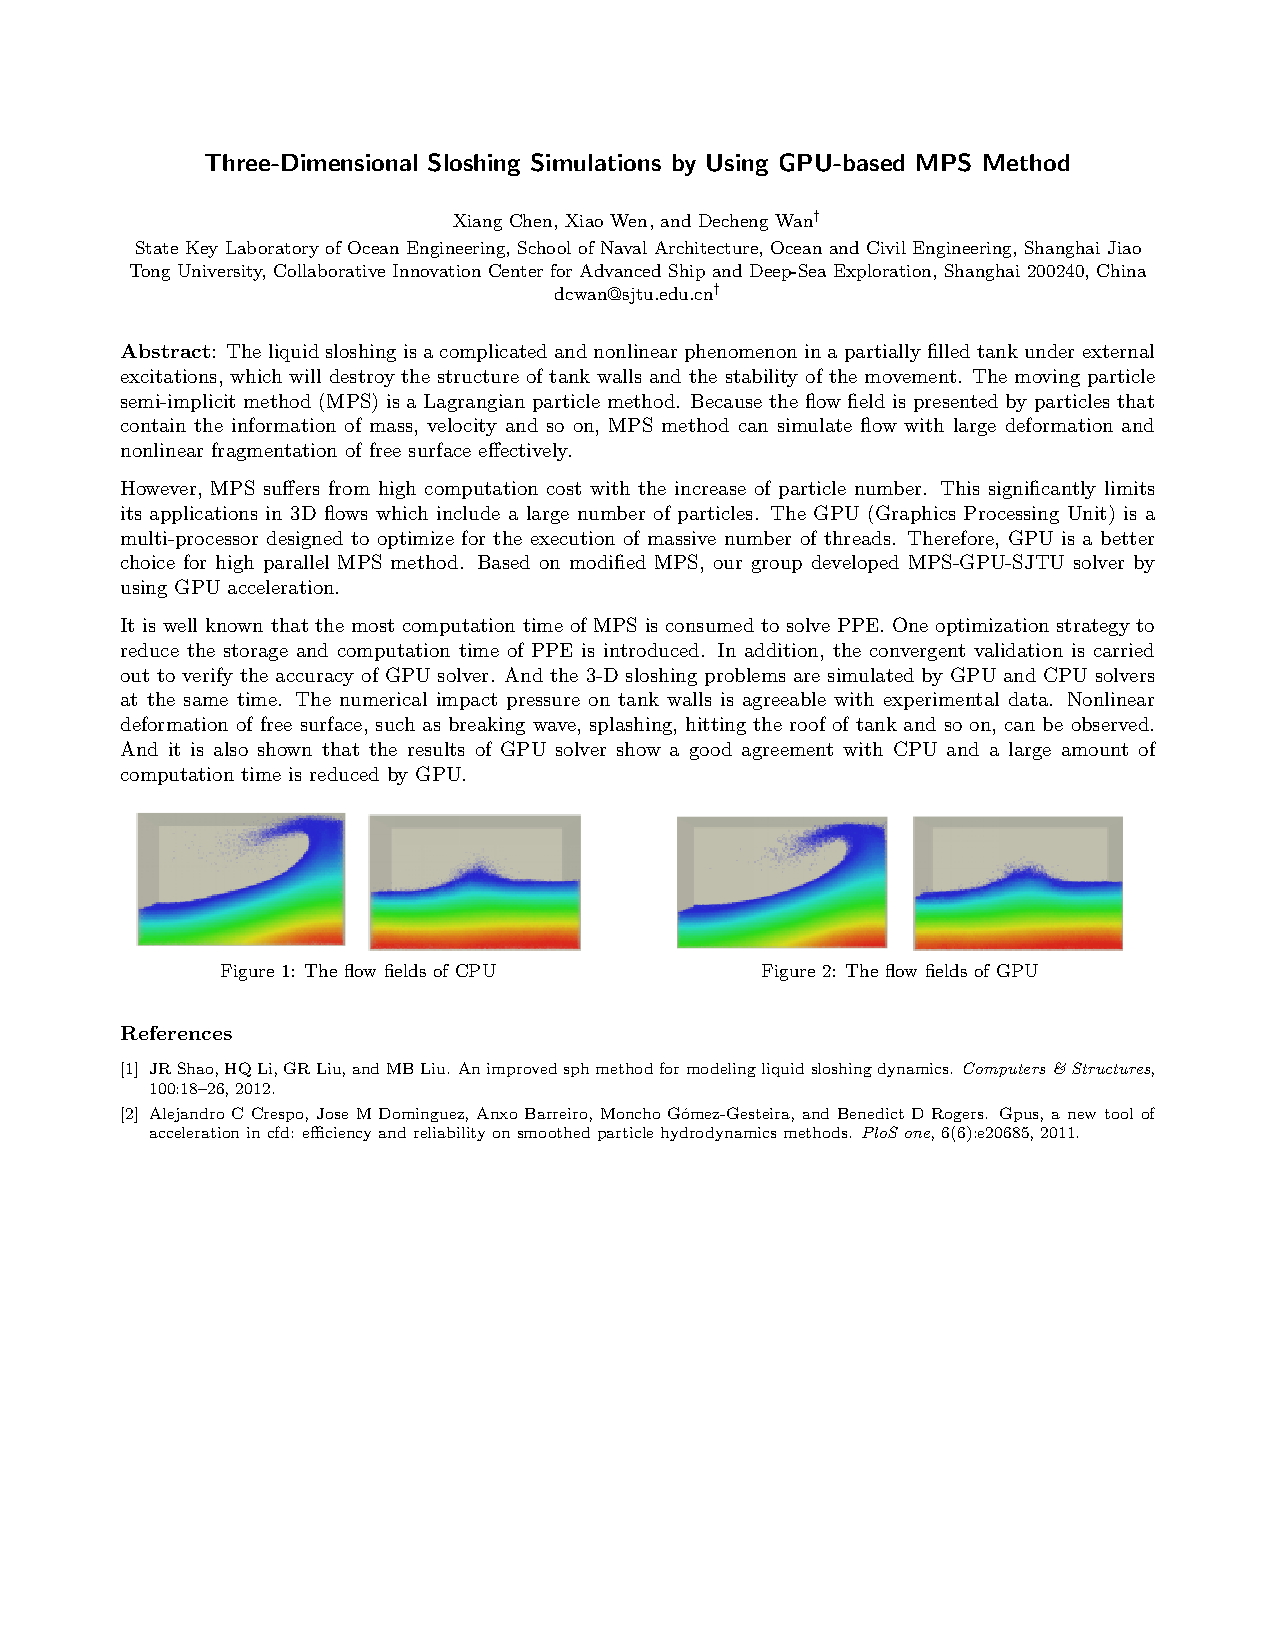
\includepdf[pages=-,pagecommand={\pagestyle{fancy}\label{9.2}},addtotoc={  
     1,subsection,1,Three-dimensional sloshing simulations by using GPU-based MPS method,p1}]{abstract/pdfs/16.pdf}
     
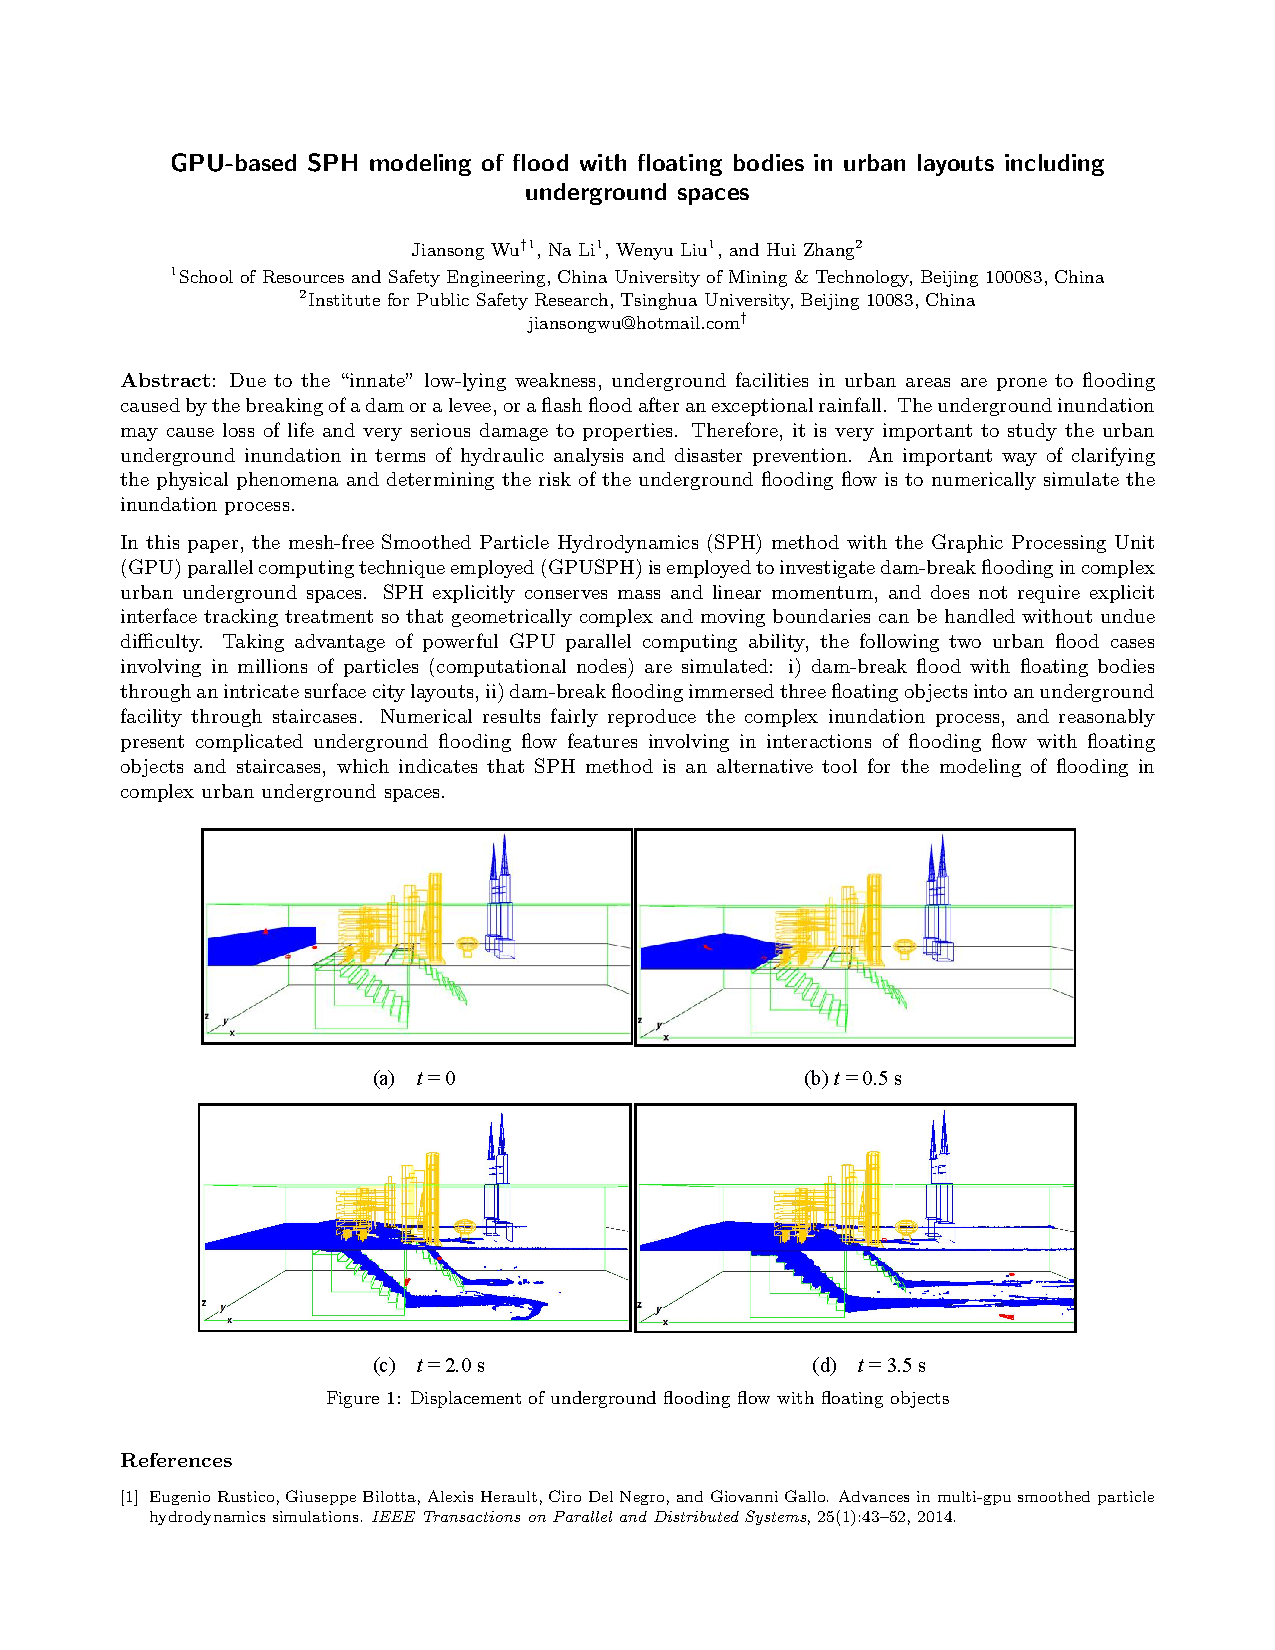
\includepdf[pages=-,pagecommand={\pagestyle{fancy}\label{9.3}},addtotoc={  
     1,subsection,1,GPU-based SPH modeling of flood with floating bodies in urban layouts including underground spaces,p1}]{abstract/pdfs/26.pdf}
%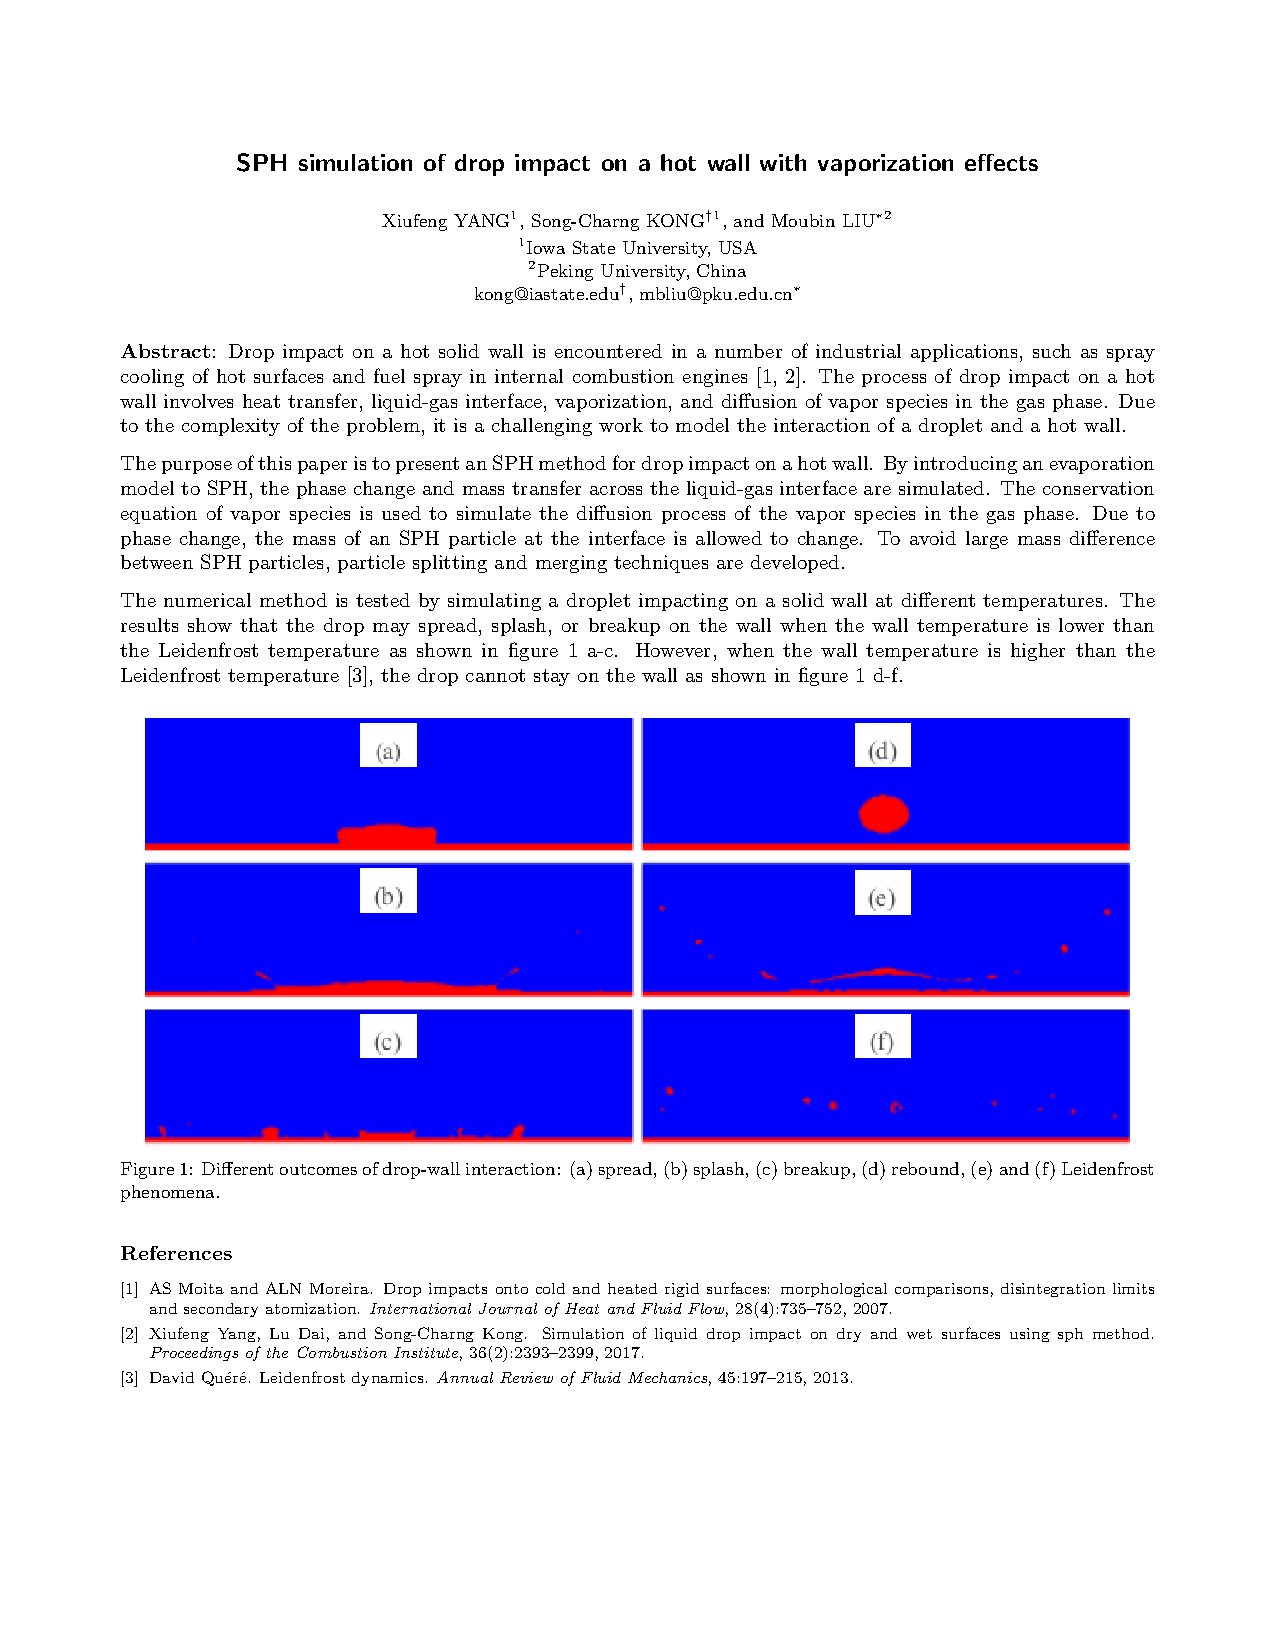
\includepdf[pages=-,pagecommand={\pagestyle{fancy}\label{9.4}},addtotoc={  
%     1,subsection,1,Improve the effectively of computational fluid dynamics work based on supercomputing cloud,p1}]{abstract/pdfs/9.pdf}



%\section{Session 10: Numerical Aspects of SPH}
%10.1: 43
%10.2: 49
%10.3: 52
%10.4: 50

\rhead{Session 10}
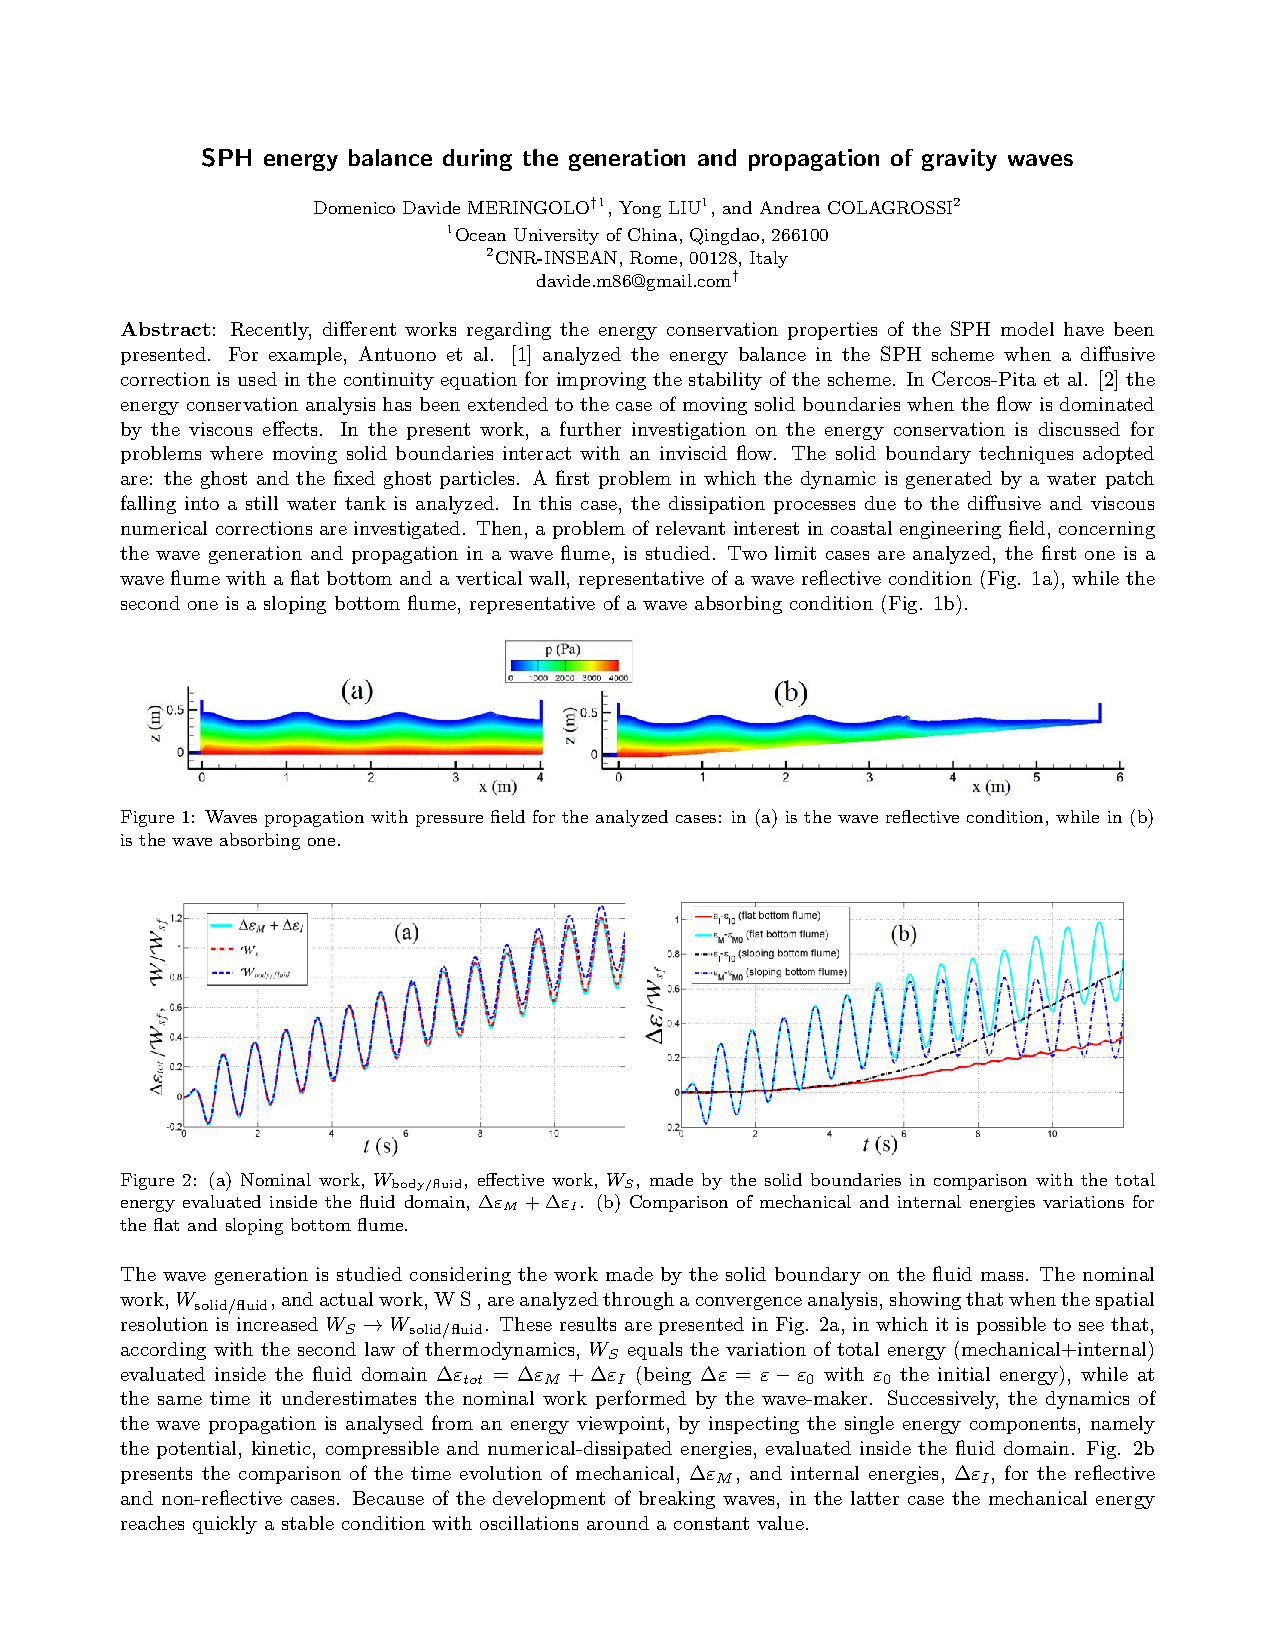
\includepdf[pages=-,pagecommand={\pagestyle{fancy}\label{10.1}},addtotoc={
     1,section,1,{~~~~~~~~Numerical Aspects of SPH},p1,   
     1,subsection,1,SPH energy balance during the generation and propagation of gravity waves,p1}]{abstract/pdfs/43.pdf}
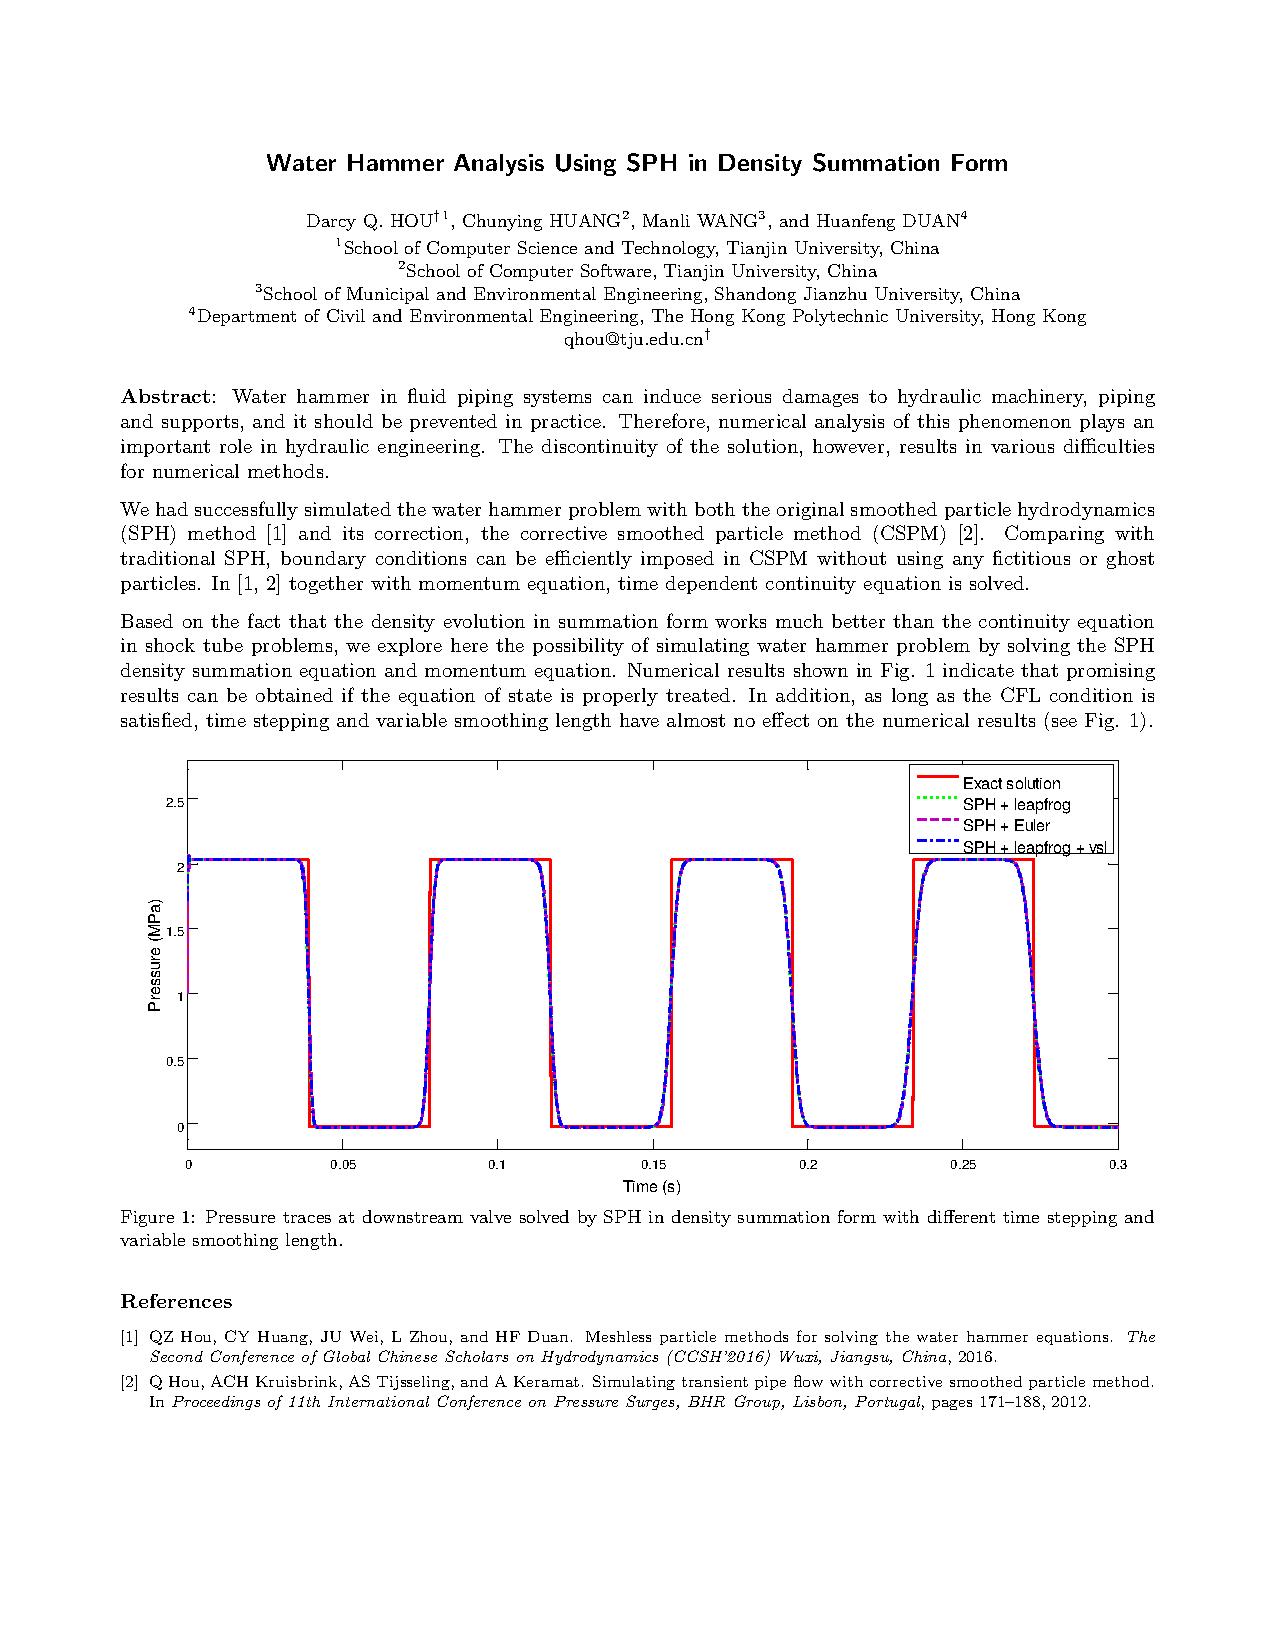
\includepdf[pages=-,pagecommand={\pagestyle{fancy}\label{10.2}},addtotoc={  
     1,subsection,1,Water hammer analysis using SPH in density summation form,p1}]{abstract/pdfs/49.pdf}
\includepdf[pages=-,pagecommand={\pagestyle{fancy}\label{10.3}},addtotoc={  
     1,subsection,1,Particle trajectory calculation in SPH,p1}]{abstract/pdfs/52.pdf}
\includepdf[pages=-,pagecommand={\pagestyle{fancy}\label{10.4}},addtotoc={  
     1,subsection,1,Simulating shock waves with corrective smoothed particle method (CSPM),p1}]{abstract/pdfs/50.pdf}



%\section{Session 11: Fluid Structure Interaction}
%11.1: 7 
%11.2: 42
%11.3: 19
%11.4: 45


\rhead{Session 11}
\includepdf[pages=-,pagecommand={\pagestyle{fancy}\label{11.1}},addtotoc={
     1,section,1,{~~~~~~~~Fluid Structure Interaction},p1,   
     1,subsection,1,SPH modeling of fluid-structure interaction (FSI),p1}]{abstract/pdfs/7.pdf}
\includepdf[pages=-,pagecommand={\pagestyle{fancy}\label{11.2}},addtotoc={  
     1,subsection,1,Numerical modeling of 2D complex movement patterns to FSI problems using smoothed particle hydrodynamics,p1}]{abstract/pdfs/42.pdf}
\includepdf[pages=-,pagecommand={\pagestyle{fancy}\label{11.3}},addtotoc={  
     1,subsection,1,Implement of the MPS-FEM coupled method for the FSI simulation of the 3-D dam-break problem,p1}]{abstract/pdfs/19.pdf}
\includepdf[pages=-,pagecommand={\pagestyle{fancy}\label{11.4}},addtotoc={  
     1,subsection,1,A new numerical method for SPH fluid-solid coupling simulation and its preliminary verification,p1}]{abstract/pdfs/45.pdf}


%\section{Session 12: Modelling of Incompressible Flows}
%12.1: 2
%12.2: 17
%12.3: 27    
%12.4: 18

\rhead{Session 12}
\includepdf[pages=-,pagecommand={\pagestyle{fancy}\label{12.1}},addtotoc={
     1,section,1,{~~~~~~~~Modelling of Incompressible Flows},p1,   
     1,subsection,1,An enhanced ISPH-SPH coupled method for incompressible fluid-elastic structure interactions,p1}]{abstract/pdfs/2.pdf}
\includepdf[pages=-,pagecommand={\pagestyle{fancy}\label{12.2}},addtotoc={  
     1,subsection,1,Interaction between solitary wave and flexible plate based on MPS-FEM coupled method,p1}]{abstract/pdfs/17.pdf}
\includepdf[pages=-,pagecommand={\pagestyle{fancy}\label{12.3}},addtotoc={  
     1,subsection,1,Modeling of single film bubble and numerical study of the plateau structure in foam system,p1}]{abstract/pdfs/27.pdf}
\includepdf[pages=-,pagecommand={\pagestyle{fancy}\label{12.4}},addtotoc={  
     1,subsection,1,Numerical simulation of Rayleigh-Taylor instability by MPS multiphase method,p1}]{abstract/pdfs/18.pdf}



%\section{Session 13: Alternative Formulations and Particle-Based Simulation Techniques}
%13.1: 35
%13.2: 56
%13.3: 13
%13.4: 23

\rhead{Session 13}
\includepdf[pages=-,pagecommand={\pagestyle{fancy}\label{13.1}},addtotoc={
     1,section,1,{~~~~~~~~Alternative Formulations and Particle-Based Simulation Techniques},p1,   
     1,subsection,1,Numerical simulation of particle collision and breakup behavior by SDPH-FVM coupling method,p1}]{abstract/pdfs/35.pdf}
\includepdf[pages=-,pagecommand={\pagestyle{fancy}\label{13.2}},addtotoc={  
     1,subsection,1,A physics evoked meshfree method,p1}]{abstract/pdfs/56.pdf}
\includepdf[pages=-,pagecommand={\pagestyle{fancy}\label{13.3}},addtotoc={  
     1,subsection,1,Suppression of non-physical voids in the finite volume particle method,p1}]{abstract/pdfs/13.pdf}
\includepdf[pages=-,pagecommand={\pagestyle{fancy}\label{13.4}},addtotoc={  
     1,subsection,1,The Hermit-type RRKPM for piezoelectric materials,p1}]{abstract/pdfs/23.pdf}

%\section{Session 14: Other applications of SPH}
%14.1: 47
%14.2: 34
%14.3: 54
%14.4: 51

\rhead{Session 14}
\includepdf[pages=-,pagecommand={\pagestyle{fancy}\label{14.1}},addtotoc={
     1,section,1,{~~~~~~~~Other applications of SPH},p1,   
     1,subsection,1,A development of a SPH model for simulation of abrasive-water-jet impacting on a metallic surface,p1}]{abstract/pdfs/47.pdf}
\includepdf[pages=-,pagecommand={\pagestyle{fancy}\label{14.2}},addtotoc={  
     1,subsection,1,SPH simulation of Couette flow with sinusoidally moving solid boundary,p1}]{abstract/pdfs/34.pdf}
\includepdf[pages=-,pagecommand={\pagestyle{fancy}\label{14.3}},addtotoc={  
     1,subsection,1,Application of particle-based computational acoustics to sound propagation and scattering,p1}]{abstract/pdfs/54.pdf}
\includepdf[pages=-,pagecommand={\pagestyle{fancy}\label{14.4}},addtotoc={  
     1,subsection,1,Image processing with the SPH method,p1}]{abstract/pdfs/51.pdf}

%\section{Session 15: Hydraulic Applications II}
%15.1: 8 
%15.2: 20
%15.3: 28
%15.4: 53

\rhead{Session 15}
\includepdf[pages=-,pagecommand={\pagestyle{fancy}\label{15.1}},addtotoc={
     1,section,1,{~~~~~~~~Hydraulic Applications II},p1,   
     1,subsection,1,Analysis of the hydrological safety of dams using numerical tools: Iber and DualSPHysics,p1}]{abstract/pdfs/8.pdf}
\includepdf[pages=-,pagecommand={\pagestyle{fancy}\label{15.2}},addtotoc={  
     1,subsection,1,Construction of two-dimensional SPH numerical wave tank,p1}]{abstract/pdfs/28.pdf}
\includepdf[pages=-,pagecommand={\pagestyle{fancy}\label{15.3}},addtotoc={  
     1,subsection,1,An SPH numerical wave-current tank,p1}]{abstract/pdfs/53.pdf}
     
     
     
\rhead{Without presentation}

\includepdf[pages=-,pagecommand={\pagestyle{fancy}}]{abstract/pdfs/32.pdf}


\chapter*{List of Participants}
\chead{}
\rhead{List of Participants}
\addcontentsline{toc}{chapter}{List of Participants} \mtcaddchapter
%\addstarredchapter{Participants}
%\chaptermark{Participants}

\renewcommand{\arraystretch}{1.2}
\vspace{-5em}
\begin{longtable}{ll}
%\hline 
A. Colagrossi&	Marine Tech. Research Inst., Italy\\ 
Aman Zhang&	Harbin Engineering University, China\\ 
Benedict D. Rogers&	University of Manchester, UK\\ 
Can Huang&	Zhejiang University, China\\ 
Chao Shi&	Xi'an Hi - Tech Institute, China\\ 
Chen Zhuang&	Hunan University, China\\ 
Chengping Rao&	Shanghai Jiao Tong University, China\\ 
Chunying Huang&	Tianjin University, China\\ 
D. Le Touze&	Ecole Centrale Nantes, France\\ 
Darcy Q. Hou&	Tianjin University, China\\ 
Domenico Davide Meringolo&	Ocean University of China, China\\ 
Feng Zhang&	Xiamen University, China\\ 
Furen Ming&	Harbin Engineering University, China\\ 
Fuzhen Chen&	Xi'an Hi - Tech Institute, China\\ 
Gang Yang&	Hunan University, China\\ 
Gaofeng Wei&	Qilu University of Technology, China\\ 
Guoxing Zhang &	Xi'an Hi - Tech Institute, China\\ 
Haiqiao Li&	North University of China, China\\ 
Haisheng Fang&	Huazhong University of Science \& Technology, China\\ 
Han Cheng&	Harbin Engineering University, China\\ 
Hongfu Qiang&	Xi'an Hi - Tech Institute, China\\ 
Hongshu Wang&	Tianjin University, China\\ 
Huabin Shi&	Tsinghua University, China\\ 
Hualin Zheng&	Xi'an Hi - Tech Institute, China\\ 
J. González-Cao&	Universidade de Vigo, Spain\\ 
J. S. Chen&	University of California San Diego, USA\\ 
J. M. Domínguez&	Universidade de Vigo, Spain\\ 
Jianqiang Chen&	China Aerodynamics Research and Development Center, China\\ 
Jiansong Wu&	China University of Mining \& Technology, China\\ 
Jiaru Shao&	Chongqing University of Technology, China\\ 
Jiayuan Shen&	Tianjin University, China\\ 
Jichao Ma&	Qilu University of Technology, China\\ 
Jie Deng&	Tianjin University, China\\ 
Jie Zhao&	Xinjiang University, China\\ 
Jingjun Li&	China Agricultural University, China\\ 
Jingyu Wang&	Northwestern Polytechnical University, China\\ 
Li Zhou&	Dalian University of Technology, China\\ 
Liangjun Wen&	China Ship Scientific Research Center, China\\ 
Liuchao Qiu&	China Agricultural University, China\\ 
Lu Wang&	Northwestern Polytechnical University, China\\ 
M. De Leffe&	Nextflow Software Nantes, France\\ 
Martin Rentschler&	ANDRITZ Hydro R\&D, Switzerland\\ 
Matthias Mimault &	James Hutton Institute, UK\\ 
Ming He&	Tianjin University, China\\ 
Mingyu Zhang&	Institute of Applied Physics and Computational Mathematics, China\\ 
Moubin Liu&	Peking University, China\\ 
Na Li&	China University of Mining \& Technology, China\\ 
Nan Qiao&	Beijing Paratera, China\\
Nathan J. Quinlan &	National University of Ireland Galway, Ireland\\ 
Pengnan Sun&	Harbin Engineering University, China\\ 
Qing Fan&	Sun Yat-sen University, China\\ 
S. Marrone&	Marine Tech. Research Inst., Italy\\ 
Sam Raymond&	Massachusetts Institute of Technology (MIT), USA\\ 
Shaohan Zhao&	Monash University, Australia\\ 
Stefano Sibilla&	University of Pavia, Italy\\ 
Ting Long&	Hunan University, China\\ 
Weizhen Kong&	Beijing Institute of Technology, China\\ 
Wenkui Shi&	China Aerodynamics Research and Development Center, China\\ 
Wenqing Hu&	Sun Yat-sen University, China\\ 
Wentao Zhang&	Institute of Mechanics, Chinese Academy of Sciences, China\\ 
Xiang Chen&	Shanghai Jiao Tong University, China\\ 
Xiangwei Dong&	China University of Petroleum, China \\ 
Xiangyu Hu&	Technical University of Munich, Germany\\ 
Xiao Wen&	Shanghai Jiao Tong University, China\\ 
Xiaohu Guo&	Science and Technology Facilities Council (STFC) , UK\\ 
Xiaojing Ma&	Xinjiang University, China\\ 
Xing Zheng&	Harbin Engineering University, China\\ 
Xinya Sun&	Xi'an Hi - Tech Institute, China\\ 
Xiufeng Yang&	Iowa State University, USA\\ 
Yanming Shen&	China Aerodynamics Research and Development Center, China\\ 
Yaxuan Xing&	Tianjin University, China\\ 
Yazhou Zhao&	Chinese Academy of Science, China\\ 
Yi An&	Institute of Mechanics, Chinese Academy of Sciences, China\\ 
Yingnan Wang&	Monash University, Australia\\ 
Yingxuan Shi&	Zhejiang University, China\\ 
Yongkang Hu&	Triangle Tire R\&D, China\\ 
Yongou Zhang&	Wuhan University of Technology, China\\ 
Youlin Zhang&	Shanghai Jiao Tong University, China\\ 
Yuantong Gu&	Queensland University of Technology, Australia\\ 
Yuma Shimizu&	Kyoto University, Japan\\ 
Zhi Zong&	Dalian University of Technology, China\\ 
Zhibo Ma&	Institute of Applied Physics and Computational Mathematics, China\\ 
Zhilang Zhang&	Peking University, China\\ 
Zhiwen Cai&	China Ship Scientific Research Center, China\\ 
Zhongguo Sun&	Xian Jiaotong University, China\\ 
Zhongyi Liu&	Huazhong University of Science \& Technology, China\\ 
%\hline 
\end{longtable}



\end{document}
